\documentclass[11pt,oneside]{book}
\usepackage[utf8]{inputenc} 
\usepackage[T1]{fontenc} % fonts to encode unicode
\usepackage{draftflag}
\usepackage{times}
\usepackage{fullpage}

\usepackage{makeidx}
\makeindex
\renewcommand{\indexname}{Author Index}

\usepackage{pdfpages}   % can also use [draft] option
\usepackage[colorlinks,
%%% EDIT TITLE: %%%%%%%%%%%%%%%%%%%%%%%%%%%%%%%%%%%%%%%%%%%%%%%%%%%%
            pdftitle={Proceedings of the First Workshop on Subword and Character Level Models in NLP},
            pdfauthor={Association for Computational Linguistics},
            %pdfsubject={...},
            %pdfkeywords={...}
           ]{hyperref}   % hyperlinked table of contents, etc.
\hypersetup{plainpages=false}  % point to papers, not preface

% for A4 size %%%%%%%%%%%%%%%%%%%%%%%%%%%%%%%%%%%%%%%%%%%%%%%%%%%
\setlength{\paperwidth}{21cm}   % A4
\setlength{\paperheight}{29.7cm}% A4
\special{papersize=21cm, 29.7cm}
\pdfpageheight\paperheight
\pdfpagewidth\paperwidth
\setlength\topmargin{-5mm} \setlength\oddsidemargin{-0cm}
\setlength\textheight{24.7cm} \setlength\textwidth{16cm}
\setlength\columnsep{0.6cm}  \newlength\titlebox \setlength\titlebox{2.00in}
\setlength\headheight{5pt}   \setlength\headsep{0pt}
\setlength\footskip{0.8cm}
\setlength\leftmargin{0.0in}
\pagestyle{plain}
%%%%%%%%%%%%%%%%%%%%%%%%%%%%%%%%%%%%%%%%%%%%%%%%%%%


\usepackage{color}
\definecolor{brown}{rgb}{0.59, 0.29, 0.0}
\newcommand{\changeurlcolor}[1]{\hypersetup{urlcolor=#1}}       
\newcommand{\citeinfo}[2]{
  \AddToShipoutPicture{%
    \setlength{\unitlength}{1mm}
    \put(105,12){\makebox(0,0){\footnotesize {\em Proceedings of the First Workshop on Subword and Character Level Models in NLP},
	\ifthenelse{\equal{#1}{#2}}{page #1}{pages #1--#2}, }
     \put(105,8){\makebox(0,0){\footnotesize Copenhagen, Denmark, September 7–11, 2017. \copyright 2017 Association for Computational Linguistics}}
  }
}

% for A4 size %%%%%%%%%%%%%%%%%%%%%%%%%%%%%%%%%%%%%%%%%%%%%%%%%%%

\newcommand{\draftframe}[1][0]{
  \AddToShipoutPicture{
    \setlength{\unitlength}{1mm}
    \put(20,25){\line(1,0){175}}
    \put(20,276){\line(1,0){175}}
    \multiput(20,256)(0,10){4}{\line(1,0){40}}
    \multiput(20,256)(0,5){8}{\line(1,0){30}}
    \multiput(20,256)(0,1){35}{\line(1,0){20}}
    \put(70,256){\makebox(0,0){20mm}}
    \put(70,266){\makebox(0,0){10mm}}
    \put(70,286){\makebox(0,0){-10mm}}

    \put(25,20){\line(0,1){271}}
    \put(186,20){\line(0,1){271}}

    \multiput(15,172)(10,0){3}{\line(0,1){53}}
    \multiput(15,172)(5,0){5}{\line(0,1){46}}
    \multiput(15,172)(1,0){20}{\line(0,1){40}}

    \put(15,232){\makebox(0,0){-10}}
    \put(35,232){\makebox(0,0){10}}
    \put(15,227){\makebox(0,0){mm}}
    \put(35,227){\makebox(0,0){mm}}

    \put(108,282){\makebox(0,0){\bf \LARGE \tt Paper ID #1}}
  }
}

%%%%%%%%%%%%%%%%%%%%%%%%%%%%%%%%%%%%%%%%%%%%%%%%%%%

\begin{document}
\pagenumbering{roman}

% -------- COVER --------

\thispagestyle{empty}
\ifthenelse{\equal{\draftflag}{1}}{\draftframe}{}
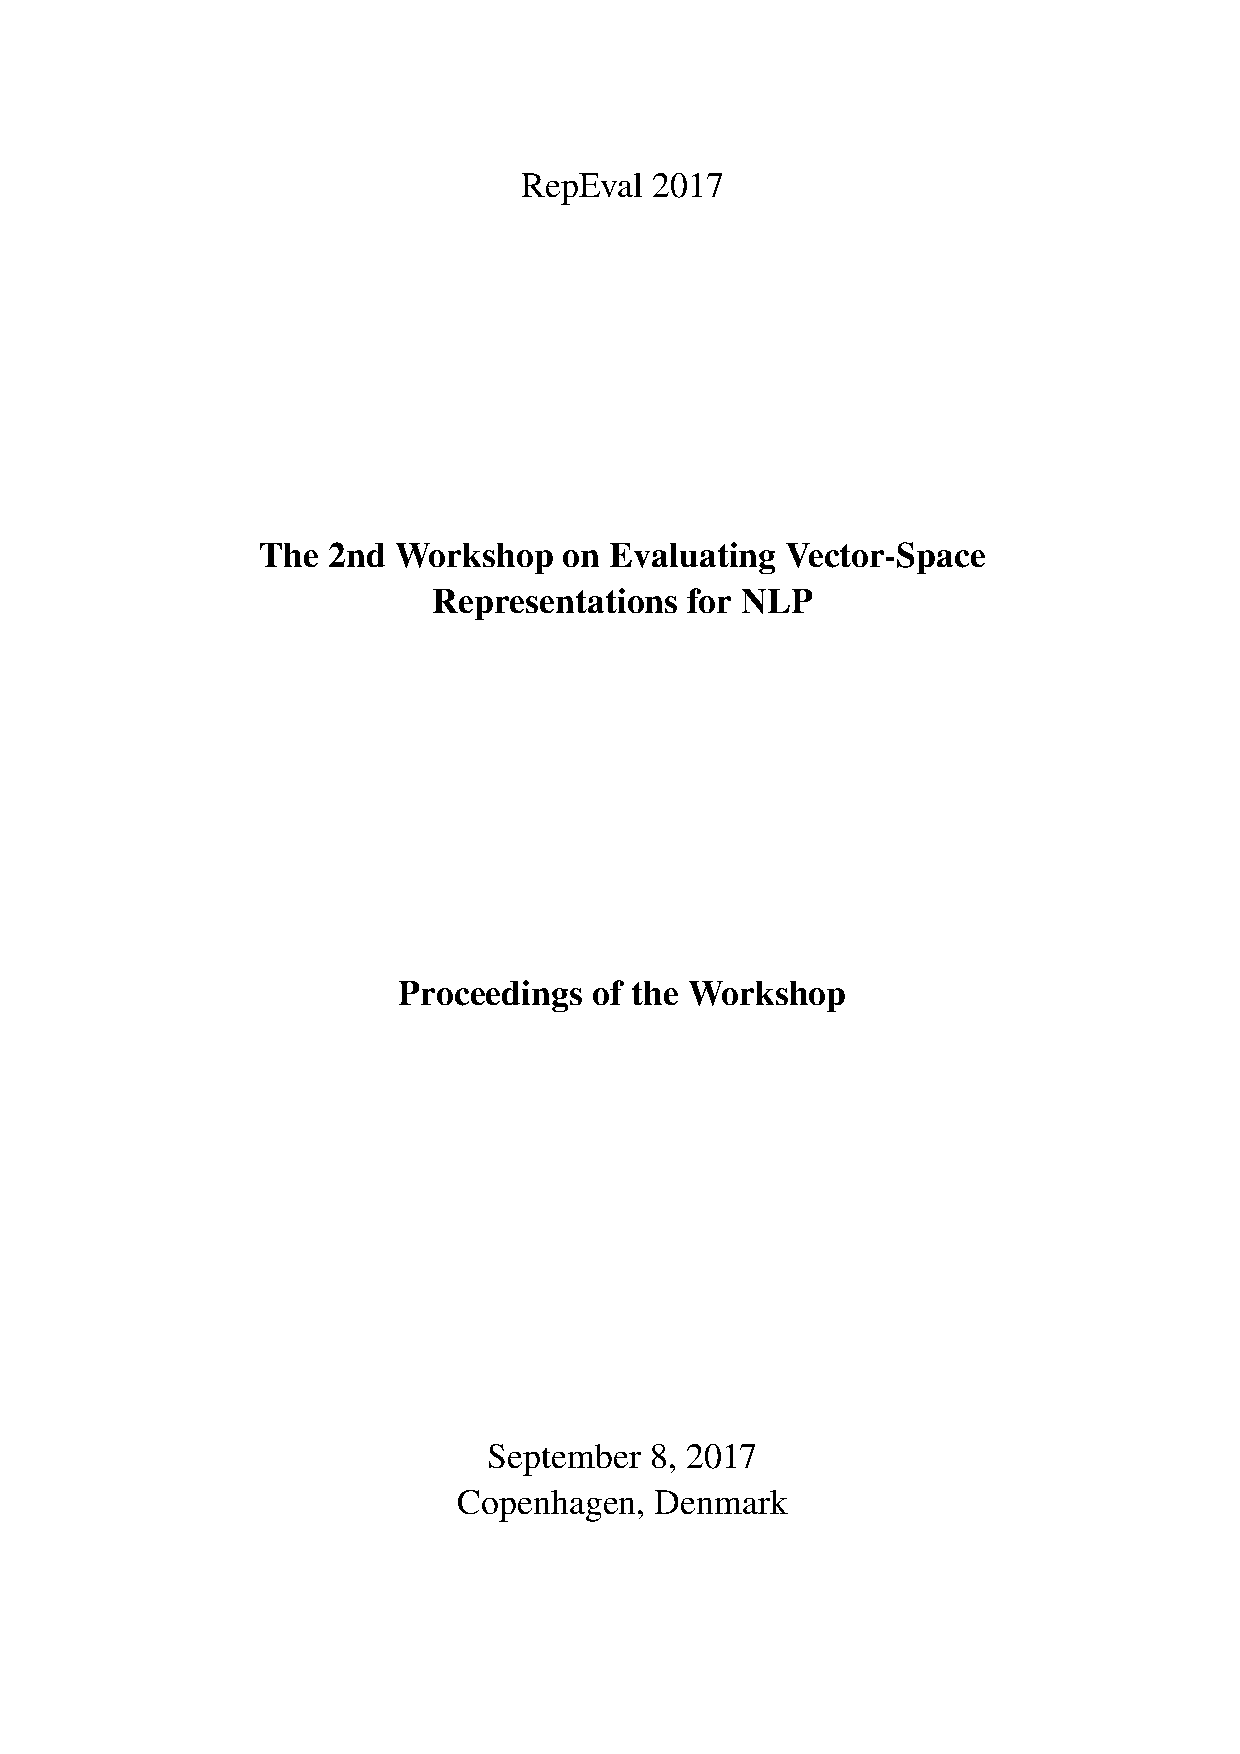
\includepdf{titlepage.pdf}

% -------- FRONT MATTER --------

\includepdfset{pages=-,clip,noautoscale,pagecommand={\thispagestyle{plain}}}

\ifthenelse{\equal{\draftflag}{1}}{\draftframe}{}
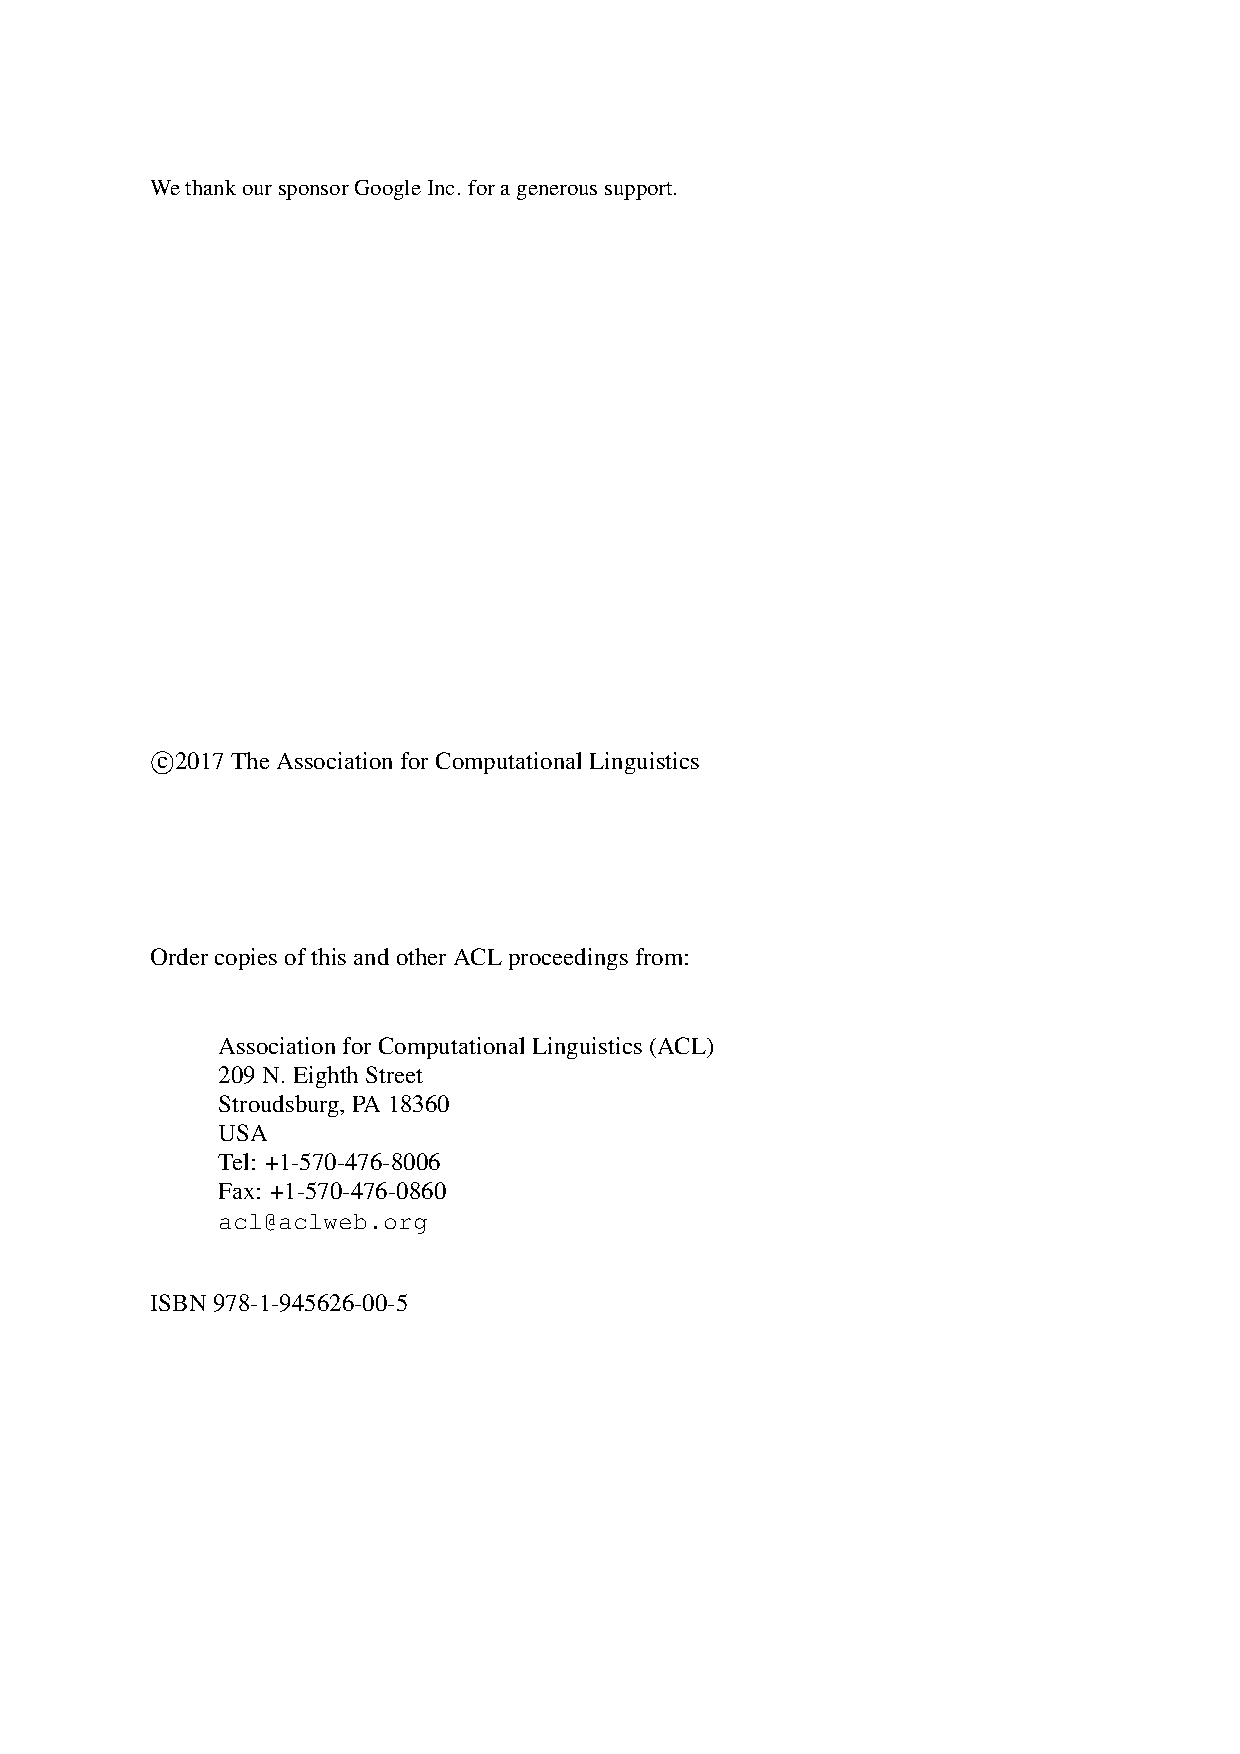
\includepdf{copyright.pdf}

\ifthenelse{\equal{\draftflag}{1}}{\draftframe}{}
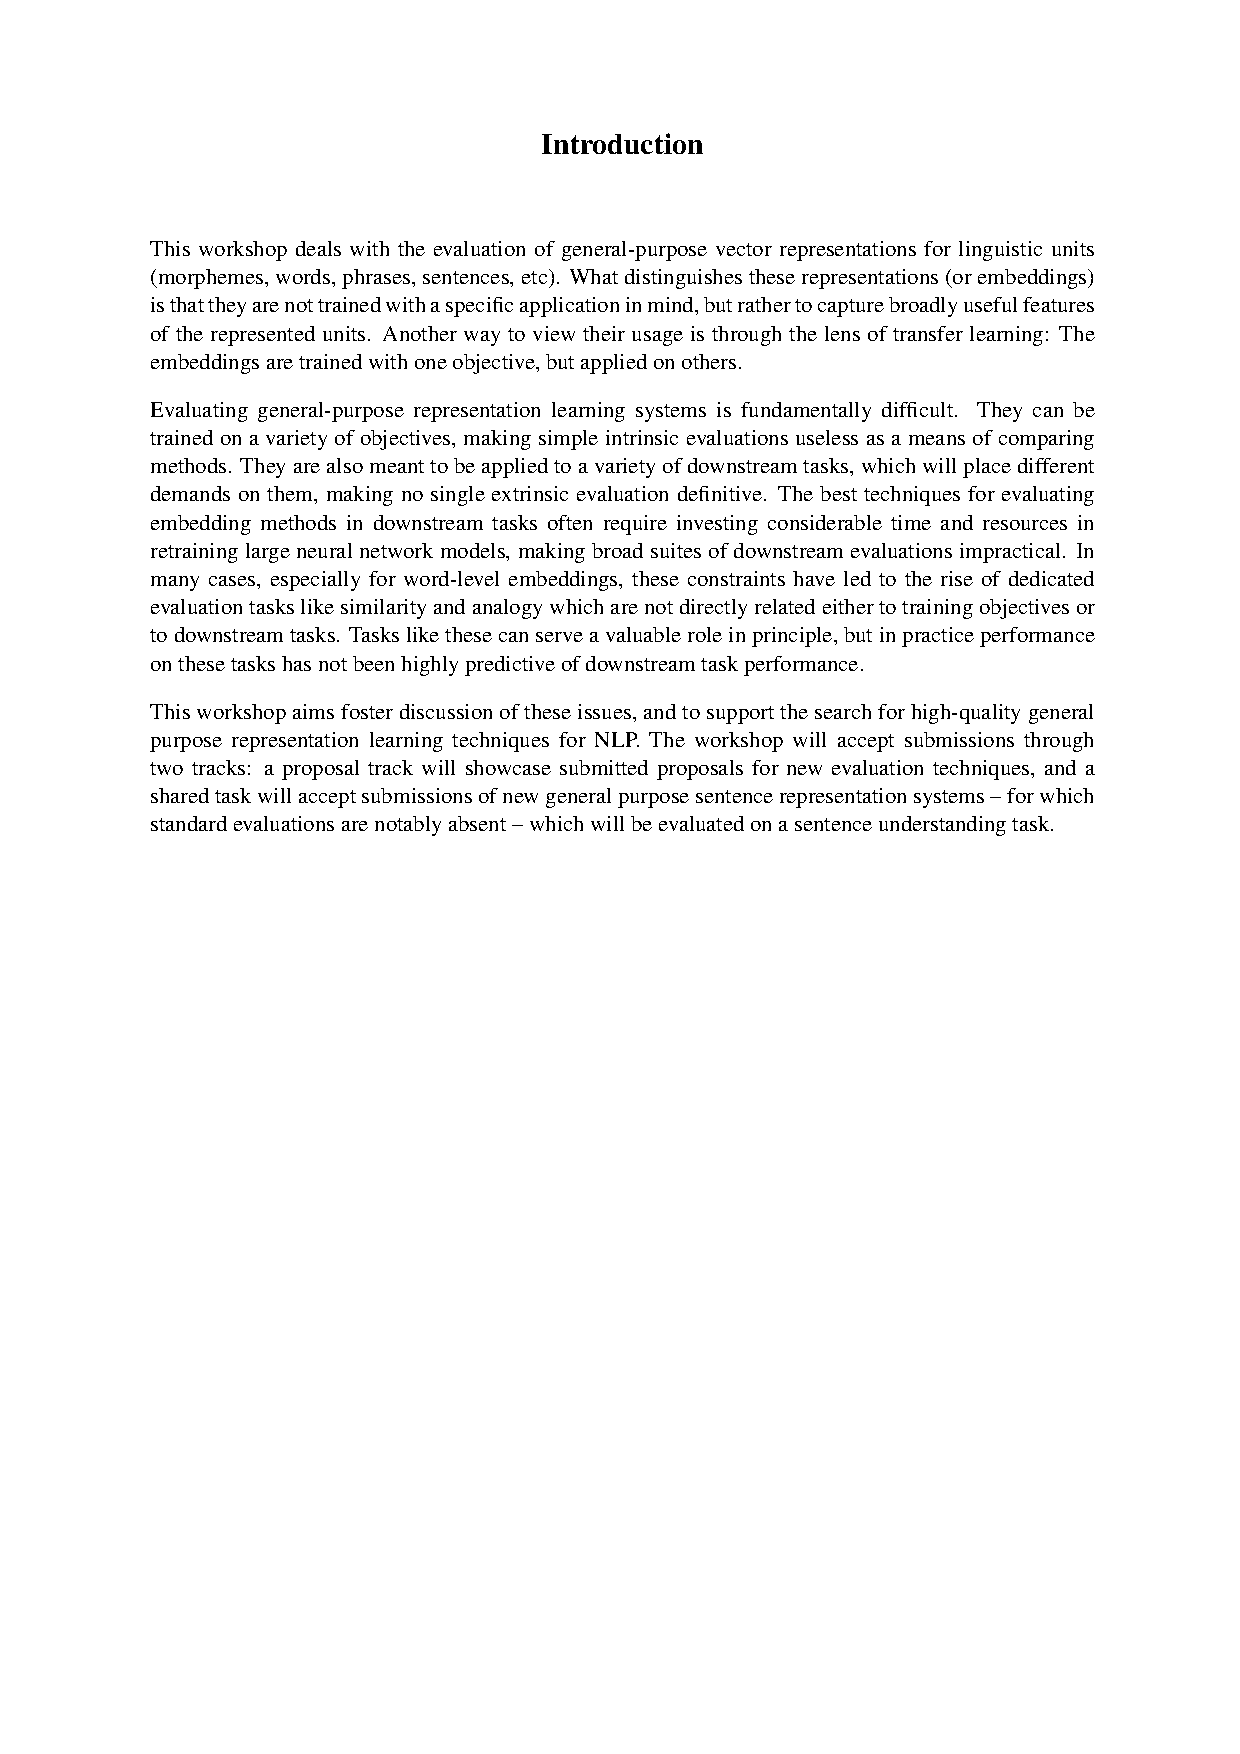
\includepdf{preface.pdf}
\ifthenelse{\isodd{\value{page}}}{}{\newpage \thispagestyle{empty} \phantom{.}}

\ifthenelse{\equal{\draftflag}{1}}{\draftframe}{}
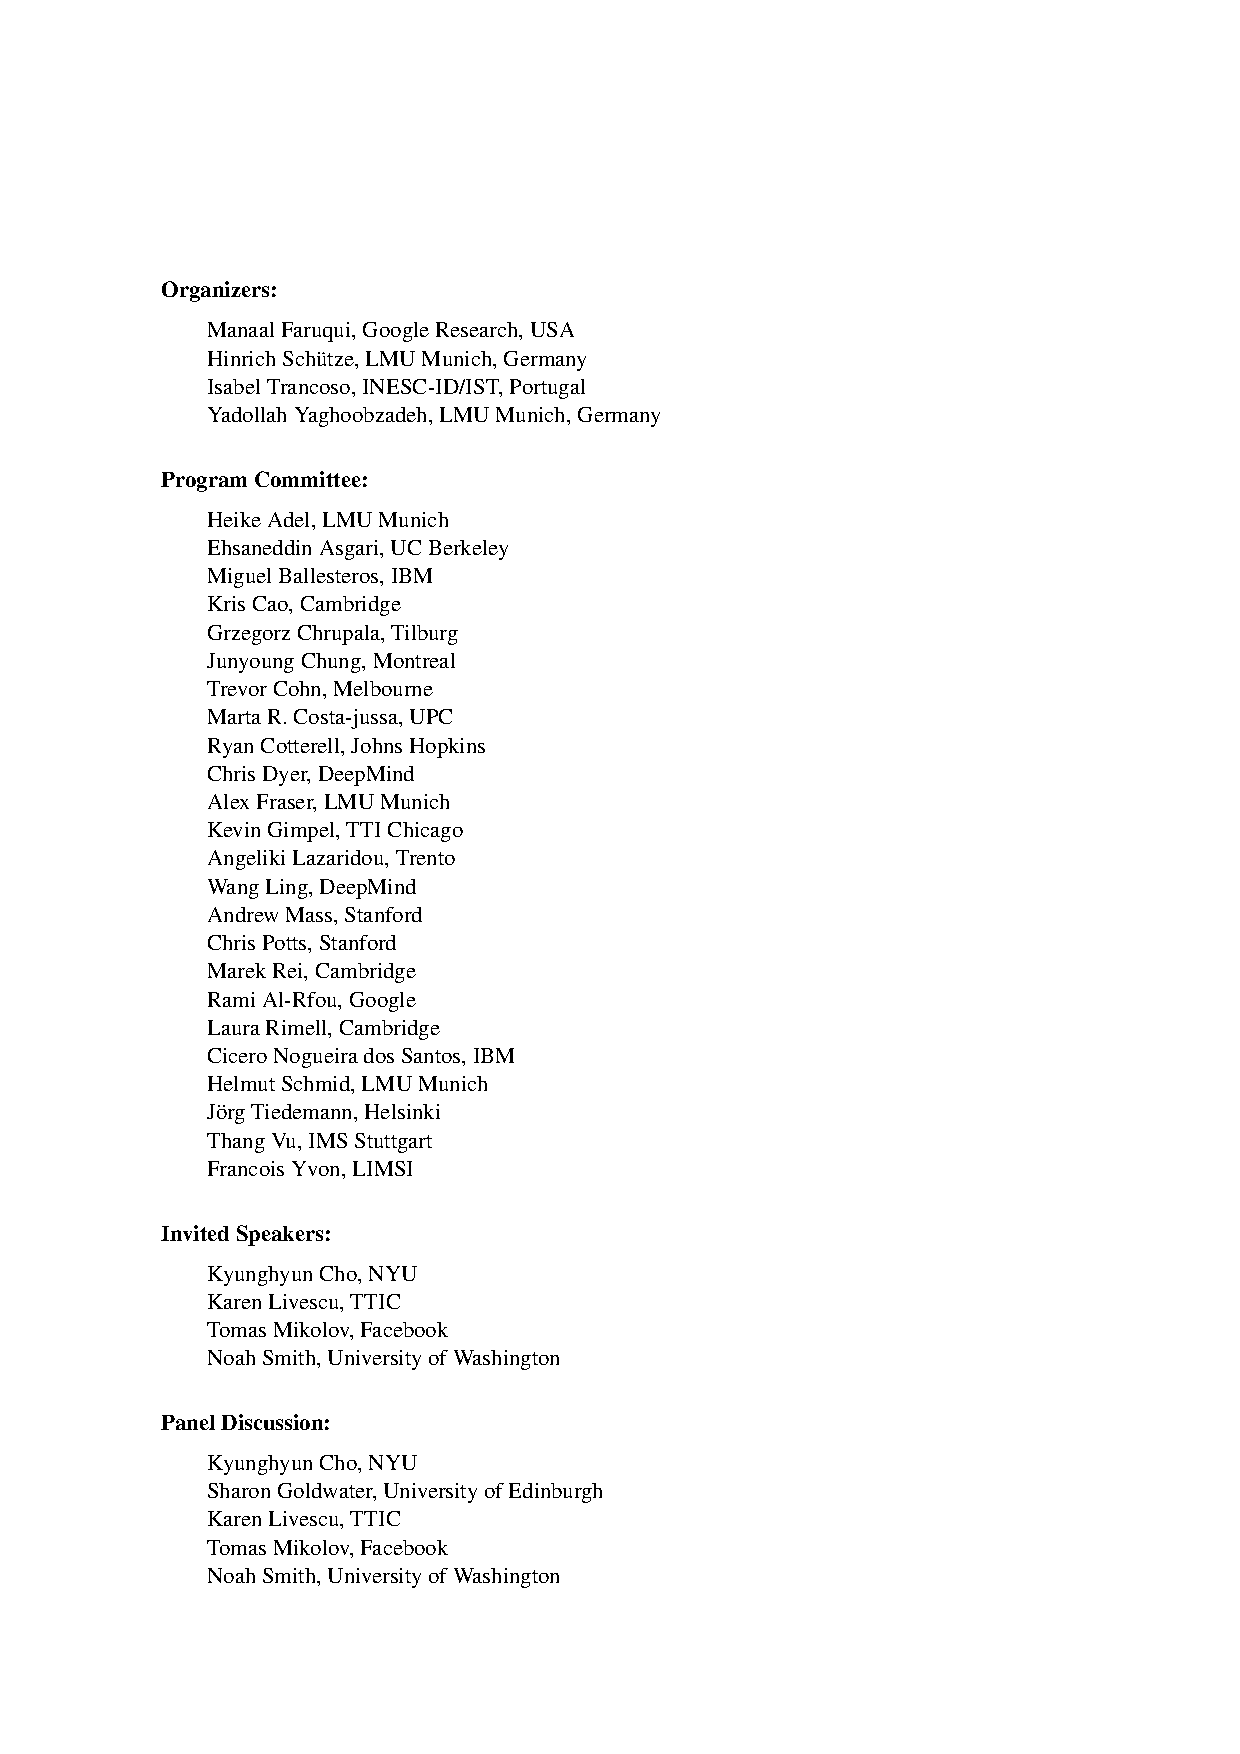
\includepdf{organizers.pdf}
\ifthenelse{\isodd{\value{page}}}{}{\newpage \thispagestyle{empty} \phantom{.}}

\ifthenelse{\equal{\draftflag}{1}}{\draftframe}{}
\setlength{\parindent}{0in}
\setlength{\parskip}{2ex}

\begin{center}
  {\Large \bf Table of Contents}
\end{center}

\vspace*{0.5cm}
\hyperlink{page.1}{\em Monolingual Phrase Alignment on Parse Forests}\samepage \\
\hspace*{7mm} Yuki Arase and Jun'ichi Tsujii\dotfill \hyperpage{1}

\hyperlink{page.12}{\em Fast(er) Exact Decoding and Global Training for Transition-Based Dependency Parsing via a Minimal Feature Set}\samepage \\
\hspace*{7mm} Tianze Shi, Liang Huang and Lillian Lee\dotfill \hyperpage{12}

\hyperlink{page.24}{\em Quasi-Second-Order Parsing for 1-Endpoint-Crossing, Pagenumber-2 Graphs}\samepage \\
\hspace*{7mm} Junjie Cao, Sheng Huang, Weiwei Sun and Xiaojun Wan\dotfill \hyperpage{24}

\hyperlink{page.35}{\em Position-aware Attention and Supervised Data Improve Slot Filling}\samepage \\
\hspace*{7mm} Yuhao Zhang, Victor Zhong, Danqi Chen, Gabor Angeli and Christopher D. Manning\dotfill \hyperpage{35}

\hyperlink{page.46}{\em Heterogeneous Supervision for Relation Extraction: A Representation Learning Approach}\samepage \\
\hspace*{7mm} Liyuan Liu, Xiang Ren, Qi Zhu, Shi Zhi, Huan Gui, Heng Ji and Jiawei Han\dotfill \hyperpage{46}

\hyperlink{page.57}{\em Integrating Order Information and Event Relation for Script Event Prediction}\samepage \\
\hspace*{7mm} Zhongqing Wang, Yue Zhang and Ching-Yun Chang\dotfill \hyperpage{57}

\hyperlink{page.68}{\em Entity Linking for Queries by Searching Wikipedia Sentences}\samepage \\
\hspace*{7mm} Chuanqi Tan, Furu Wei, Pengjie Ren, Weifeng Lv and Ming Zhou\dotfill \hyperpage{68}

\hyperlink{page.78}{\em Train-O-Matic: Large-Scale Supervised Word Sense Disambiguation in Multiple Languages without Manual Training Data}\samepage \\
\hspace*{7mm} Tommaso Pasini and Roberto Navigli\dotfill \hyperpage{78}

\hyperlink{page.89}{\em Universal Semantic Parsing}\samepage \\
\hspace*{7mm} Siva Reddy, Oscar T\"{a}ckstr\"{o}m, Slav Petrov, Mark Steedman and Mirella Lapata\dotfill \hyperpage{89}

\hyperlink{page.102}{\em Mimicking Word Embeddings using Subword RNNs}\samepage \\
\hspace*{7mm} Yuval Pinter, Robert Guthrie and Jacob Eisenstein\dotfill \hyperpage{102}

\hyperlink{page.113}{\em Past, Present, Future: A Computational Investigation of the Typology of Tense in 1000 Languages}\samepage \\
\hspace*{7mm} Ehsaneddin Asgari and Hinrich Sch\"{u}tze\dotfill \hyperpage{113}

\hyperlink{page.125}{\em Neural Machine Translation with Source-Side Latent Graph Parsing}\samepage \\
\hspace*{7mm} Kazuma Hashimoto and Yoshimasa Tsuruoka\dotfill \hyperpage{125}

\hyperlink{page.136}{\em Neural Machine Translation with Word Predictions}\samepage \\
\hspace*{7mm} Rongxiang Weng, Shujian Huang, Zaixiang Zheng, XIN-YU DAI and Jiajun CHEN\dotfill \hyperpage{136}

\hyperlink{page.146}{\em Towards Decoding as Continuous Optimisation in Neural Machine Translation}\samepage \\
\hspace*{7mm} Cong Duy Vu Hoang, Gholamreza Haffari and Trevor Cohn\dotfill \hyperpage{146}

\hyperlink{page.157}{\em Where is Misty? Interpreting Spatial Descriptors by Modeling Regions in Space}\samepage \\
\hspace*{7mm} Nikita Kitaev and Dan Klein\dotfill \hyperpage{157}

\hyperlink{page.167}{\em Continuous Representation of Location for Geolocation and Lexical Dialectology using Mixture Density Networks}\samepage \\
\hspace*{7mm} Afshin Rahimi, Timothy Baldwin and Trevor Cohn\dotfill \hyperpage{167}

\hyperlink{page.177}{\em Obj2Text: Generating Visually Descriptive Language from Object Layouts}\samepage \\
\hspace*{7mm} Xuwang Yin and Vicente Ordonez\dotfill \hyperpage{177}

\hyperlink{page.188}{\em End-to-end Neural Coreference Resolution}\samepage \\
\hspace*{7mm} Kenton Lee, Luheng He, Mike Lewis and Luke Zettlemoyer\dotfill \hyperpage{188}

\hyperlink{page.198}{\em Neural Net Models of Open-domain Discourse Coherence}\samepage \\
\hspace*{7mm} Jiwei Li and Dan Jurafsky\dotfill \hyperpage{198}

\hyperlink{page.210}{\em Affinity-Preserving Random Walk for Multi-Document Summarization}\samepage \\
\hspace*{7mm} Kexiang Wang, Tianyu Liu, Zhifang Sui and Baobao Chang\dotfill \hyperpage{210}

\hyperlink{page.221}{\em A Mention-Ranking Model for Abstract Anaphora Resolution}\samepage \\
\hspace*{7mm} Ana Marasovic, Leo Born, Juri Opitz and Anette Frank\dotfill \hyperpage{221}

\hyperlink{page.233}{\em Hierarchical Embeddings for Hypernymy Detection and Directionality}\samepage \\
\hspace*{7mm} Kim Anh Nguyen, Maximilian K\"{o}per, Sabine Schulte im Walde and Ngoc Thang Vu\dotfill \hyperpage{233}

\hyperlink{page.244}{\em Ngram2vec: Learning Improved Word Representations from Ngram Co-occurrence Statistics}\samepage \\
\hspace*{7mm} Zhe Zhao, Tao Liu, Shen Li, Bofang Li and Xiaoyong Du\dotfill \hyperpage{244}

\hyperlink{page.254}{\em Dict2vec : Learning Word Embeddings using Lexical Dictionaries}\samepage \\
\hspace*{7mm} Julien Tissier, Christopher Gravier and Amaury Habrard\dotfill \hyperpage{254}

\hyperlink{page.264}{\em Learning Chinese Word Representations From Glyphs Of Characters}\samepage \\
\hspace*{7mm} Tzu-ray Su and Hung-yi Lee\dotfill \hyperpage{264}

\hyperlink{page.274}{\em Learning Paraphrastic Sentence Embeddings from Back-Translated Bitext}\samepage \\
\hspace*{7mm} John Wieting, Jonathan Mallinson and Kevin Gimpel\dotfill \hyperpage{274}

\hyperlink{page.286}{\em Joint Embeddings of Chinese Words, Characters, and Fine-grained Subcharacter Components}\samepage \\
\hspace*{7mm} Jinxing Yu, Xun Jian, Hao Xin and Yangqiu Song\dotfill \hyperpage{286}

\hyperlink{page.292}{\em Exploiting Morphological Regularities in Distributional Word Representations}\samepage \\
\hspace*{7mm} Arihant Gupta, Syed Sarfaraz Akhtar, Avijit Vajpayee, Arjit Srivastava, Madan Gopal Jhanwar and Manish Shrivastava\dotfill \hyperpage{292}

\hyperlink{page.298}{\em Exploiting Word Internal Structures for Generic Chinese Sentence Representation}\samepage \\
\hspace*{7mm} Shaonan Wang, Jiajun Zhang and Chengqing Zong\dotfill \hyperpage{298}

\hyperlink{page.304}{\em High-risk learning: acquiring new word vectors from tiny data}\samepage \\
\hspace*{7mm} Aur\'{e}lie Herbelot and Marco Baroni\dotfill \hyperpage{304}

\hyperlink{page.310}{\em Word Embeddings based on Fixed-Size Ordinally Forgetting Encoding}\samepage \\
\hspace*{7mm} Joseph Sanu, Mingbin Xu, Hui Jiang and Quan Liu\dotfill \hyperpage{310}

\hyperlink{page.316}{\em VecShare: A Framework for Sharing Word Representation Vectors}\samepage \\
\hspace*{7mm} Jared Fernandez, Zhaocheng Yu and Doug Downey\dotfill \hyperpage{316}

\hyperlink{page.321}{\em Word Re-Embedding via Manifold Dimensionality Retention}\samepage \\
\hspace*{7mm} Souleiman Hasan and Edward Curry\dotfill \hyperpage{321}

\hyperlink{page.327}{\em MUSE: Modularizing Unsupervised Sense Embeddings}\samepage \\
\hspace*{7mm} Guang-He Lee and Yun-Nung Chen\dotfill \hyperpage{327}

\hyperlink{page.338}{\em Reporting Score Distributions Makes a Difference: Performance Study of LSTM-networks for Sequence Tagging}\samepage \\
\hspace*{7mm} Nils Reimers and Iryna Gurevych\dotfill \hyperpage{338}

\hyperlink{page.349}{\em Learning What's Easy: Fully Differentiable Neural Easy-First Taggers}\samepage \\
\hspace*{7mm} Andr\'{e} F. T. Martins and Julia Kreutzer\dotfill \hyperpage{349}

\hyperlink{page.361}{\em Incremental Skip-gram Model with Negative Sampling}\samepage \\
\hspace*{7mm} Nobuhiro Kaji and Hayato Kobayashi\dotfill \hyperpage{361}

\hyperlink{page.370}{\em Learning to select data for transfer learning with Bayesian Optimization}\samepage \\
\hspace*{7mm} Sebastian Ruder and Barbara Plank\dotfill \hyperpage{370}

\hyperlink{page.381}{\em Unsupervised Pretraining for Sequence to Sequence Learning}\samepage \\
\hspace*{7mm} Prajit Ramachandran, Peter Liu and Quoc Le\dotfill \hyperpage{381}

\hyperlink{page.390}{\em Efficient Attention using a Fixed-Size Memory Representation}\samepage \\
\hspace*{7mm} Denny Britz, Melody Guan and Minh-Thang Luong\dotfill \hyperpage{390}

\hyperlink{page.399}{\em Rotated Word Vector Representations and their Interpretability}\samepage \\
\hspace*{7mm} Sungjoon Park, JinYeong Bak and Alice Oh\dotfill \hyperpage{399}

\hyperlink{page.410}{\em A causal framework for explaining the predictions of black-box sequence-to-sequence models}\samepage \\
\hspace*{7mm} David Alvarez-Melis and Tommi Jaakkola\dotfill \hyperpage{410}

\hyperlink{page.420}{\em Piecewise Latent Variables for Neural Variational Text Processing}\samepage \\
\hspace*{7mm} Iulian Vlad Serban, Alexander G. Ororbia, Joelle Pineau and Aaron Courville\dotfill \hyperpage{420}

\hyperlink{page.431}{\em Learning the Structure of Variable-Order CRFs: a finite-state perspective}\samepage \\
\hspace*{7mm} Thomas Lavergne and Fran\c{c}ois Yvon\dotfill \hyperpage{431}

\hyperlink{page.438}{\em Sparse Communication for Distributed Gradient Descent}\samepage \\
\hspace*{7mm} Alham Fikri Aji and Kenneth Heafield\dotfill \hyperpage{438}

\hyperlink{page.444}{\em A Joint Many-Task Model: Growing a Neural Network for Multiple NLP Tasks}\samepage \\
\hspace*{7mm} Kazuma Hashimoto, caiming xiong, Yoshimasa Tsuruoka and Richard Socher\dotfill \hyperpage{444}

\hyperlink{page.455}{\em Why ADAGRAD Fails for Online Topic Modeling}\samepage \\
\hspace*{7mm} You Lu, Jeffrey Lund and Jordan Boyd-Graber\dotfill \hyperpage{455}

\hyperlink{page.461}{\em Recurrent Attention Network on Memory for Aspect Sentiment Analysis}\samepage \\
\hspace*{7mm} Peng Chen, Zhongqian Sun, Lidong Bing and Wei Yang\dotfill \hyperpage{461}

\hyperlink{page.471}{\em A Cognition Based Attention Model for Sentiment Analysis}\samepage \\
\hspace*{7mm} Yunfei Long, Lu Qin, Rong Xiang, Minglei Li and Chu-Ren Huang\dotfill \hyperpage{471}

\hyperlink{page.481}{\em Author-aware Aspect Topic Sentiment Model to Retrieve Supporting Opinions from Reviews}\samepage \\
\hspace*{7mm} Lahari Poddar, Wynne Hsu and Mong Li Lee\dotfill \hyperpage{481}

\hyperlink{page.491}{\em Magnets for Sarcasm: Making Sarcasm Detection Timely, Contextual and Very Personal}\samepage \\
\hspace*{7mm} Aniruddha Ghosh and Tony Veale\dotfill \hyperpage{491}

\hyperlink{page.501}{\em Identifying Humor in Reviews using Background Text Sources}\samepage \\
\hspace*{7mm} Alex Morales and Chengxiang Zhai\dotfill \hyperpage{501}

\hyperlink{page.511}{\em Sentiment Lexicon Construction with Representation Learning Based on Hierarchical Sentiment Supervision}\samepage \\
\hspace*{7mm} Leyi Wang and Rui Xia\dotfill \hyperpage{511}

\hyperlink{page.520}{\em Towards a Universal Sentiment Classifier in Multiple languages}\samepage \\
\hspace*{7mm} Kui Xu and Xiaojun Wan\dotfill \hyperpage{520}

\hyperlink{page.530}{\em Capturing User and Product Information for Document Level Sentiment Analysis with Deep Memory Network}\samepage \\
\hspace*{7mm} Zi-Yi Dou\dotfill \hyperpage{530}

\hyperlink{page.536}{\em Identifying and Tracking Sentiments and Topics from Social Media Texts during Natural Disasters}\samepage \\
\hspace*{7mm} Min Yang, Jincheng Mei, Heng Ji, zhao wei, Zhou Zhao and Xiaojun Chen\dotfill \hyperpage{536}

\hyperlink{page.543}{\em Refining Word Embeddings for Sentiment Analysis}\samepage \\
\hspace*{7mm} Liang-Chih Yu, Jin Wang, K. Robert Lai and Xuejie Zhang\dotfill \hyperpage{543}

\hyperlink{page.549}{\em A Multilayer Perceptron based Ensemble Technique for Fine-grained Financial Sentiment Analysis}\samepage \\
\hspace*{7mm} Md Shad Akhtar, Abhishek Kumar, Deepanway Ghosal, Asif Ekbal and Pushpak Bhattacharyya\dotfill \hyperpage{549}

\hyperlink{page.556}{\em Sentiment Intensity Ranking among Adjectives Using Sentiment Bearing Word Embeddings}\samepage \\
\hspace*{7mm} Raksha Sharma, Arpan Somani, Lakshya Kumar and Pushpak Bhattacharyya\dotfill \hyperpage{556}

\hyperlink{page.562}{\em Sentiment Lexicon Expansion Based on Neural PU Learning, Double Dictionary Lookup, and Polarity Association}\samepage \\
\hspace*{7mm} Yasheng Wang, Yang Zhang and Bing Liu\dotfill \hyperpage{562}

\hyperlink{page.573}{\em DeepPath: A Reinforcement Learning Method for Knowledge Graph Reasoning}\samepage \\
\hspace*{7mm} Wenhan Xiong, Thien Hoang and William Yang Wang\dotfill \hyperpage{573}

\hyperlink{page.583}{\em Task-Oriented Query Reformulation with Reinforcement Learning}\samepage \\
\hspace*{7mm} Rodrigo Nogueira and Kyunghyun Cho\dotfill \hyperpage{583}

\hyperlink{page.593}{\em Sentence Simplification with Deep Reinforcement Learning}\samepage \\
\hspace*{7mm} Xingxing Zhang and Mirella Lapata\dotfill \hyperpage{593}

\hyperlink{page.604}{\em Learning how to Active Learn: A Deep Reinforcement Learning Approach}\samepage \\
\hspace*{7mm} Meng Fang, Yuan Li and Trevor Cohn\dotfill \hyperpage{604}

\hyperlink{page.615}{\em Split and Rephrase}\samepage \\
\hspace*{7mm} Shashi Narayan, Claire Gardent, Shay B. Cohen and Anastasia Shimorina\dotfill \hyperpage{615}

\hyperlink{page.626}{\em Neural Response Generation via GAN with an Approximate Embedding Layer}\samepage \\
\hspace*{7mm} Zhen Xu, Bingquan Liu, Baoxun Wang, Chengjie SUN, Xiaolong Wang, Zhuoran Wang and Chao Qi\dotfill \hyperpage{626}

\hyperlink{page.636}{\em A Hybrid Convolutional Variational Autoencoder for Text Generation}\samepage \\
\hspace*{7mm} Stanislau Semeniuta, Aliaksei Severyn and Erhardt Barth\dotfill \hyperpage{636}

\hyperlink{page.647}{\em Filling the Blanks (hint: plural noun) for Mad Libs Humor}\samepage \\
\hspace*{7mm} Nabil Hossain, John Krumm, Lucy Vanderwende, Eric Horvitz and Henry Kautz\dotfill \hyperpage{647}

\hyperlink{page.657}{\em Measuring Thematic Fit with Distributional Feature Overlap}\samepage \\
\hspace*{7mm} Enrico Santus, Emmanuele Chersoni, Alessandro Lenci and Philippe Blache\dotfill \hyperpage{657}

\hyperlink{page.668}{\em SCDV : Sparse Composite Document Vectors using soft clustering over distributional representations}\samepage \\
\hspace*{7mm} Dheeraj Mekala, Vivek Gupta, Bhargavi Paranjape and Harish Karnick\dotfill \hyperpage{668}

\hyperlink{page.679}{\em Supervised Learning of Universal Sentence Representations from Natural Language Inference Data}\samepage \\
\hspace*{7mm} Alexis Conneau, Douwe Kiela, Holger Schwenk, Lo\"{i}c Barrault and Antoine Bordes\dotfill \hyperpage{679}

\hyperlink{page.690}{\em Determining Semantic Textual Similarity using Natural Deduction Proofs}\samepage \\
\hspace*{7mm} Hitomi Yanaka, Koji Mineshima, Pascual Mart\'{i}nez-G\'{o}mez and Daisuke Bekki\dotfill \hyperpage{690}

\hyperlink{page.701}{\em Multi-Grained Chinese Word Segmentation}\samepage \\
\hspace*{7mm} Chen Gong, Zhenghua Li, Min Zhang and Xinzhou Jiang\dotfill \hyperpage{701}

\hyperlink{page.713}{\em Don't Throw Those Morphological Analyzers Away Just Yet: Neural Morphological Disambiguation for Arabic}\samepage \\
\hspace*{7mm} Nasser Zalmout and Nizar Habash\dotfill \hyperpage{713}

\hyperlink{page.723}{\em Paradigm Completion for Derivational Morphology}\samepage \\
\hspace*{7mm} Ryan Cotterell, Ekaterina Vylomova, Huda Khayrallah, Christo Kirov and David Yarowsky\dotfill \hyperpage{723}

\hyperlink{page.730}{\em A Sub-Character Architecture for Korean Language Processing}\samepage \\
\hspace*{7mm} Karl Stratos\dotfill \hyperpage{730}

\hyperlink{page.736}{\em Do LSTMs really work so well for PoS tagging? -- A replication study}\samepage \\
\hspace*{7mm} Tobias Horsmann and Torsten Zesch\dotfill \hyperpage{736}

\hyperlink{page.746}{\em The Labeled Segmentation of Printed Books}\samepage \\
\hspace*{7mm} Lara McConnaughey, Jennifer Dai and David Bamman\dotfill \hyperpage{746}

\hyperlink{page.757}{\em Cross-lingual Character-Level Neural Morphological Tagging}\samepage \\
\hspace*{7mm} Ryan Cotterell and Georg Heigold\dotfill \hyperpage{757}

\hyperlink{page.769}{\em Word-Context Character Embeddings for Chinese Word Segmentation}\samepage \\
\hspace*{7mm} Hao Zhou, Zhenting Yu, Yue Zhang, Shujian Huang, XIN-YU DAI and Jiajun Chen\dotfill \hyperpage{769}

\hyperlink{page.776}{\em Segmentation-Free Word Embedding for Unsegmented Languages}\samepage \\
\hspace*{7mm} Takamasa Oshikiri\dotfill \hyperpage{776}

\hyperlink{page.782}{\em From Textbooks to Knowledge: A Case Study in Harvesting Axiomatic Knowledge from Textbooks to Solve Geometry Problems}\samepage \\
\hspace*{7mm} Mrinmaya Sachan, Kumar Dubey and Eric Xing\dotfill \hyperpage{782}

\hyperlink{page.794}{\em RACE: Large-scale ReAding Comprehension Dataset From Examinations}\samepage \\
\hspace*{7mm} Guokun Lai, Qizhe Xie, Hanxiao Liu, Yiming Yang and Eduard Hovy\dotfill \hyperpage{794}

\hyperlink{page.804}{\em Beyond Sentential Semantic Parsing: Tackling the Math SAT with a Cascade of Tree Transducers}\samepage \\
\hspace*{7mm} Mark Hopkins, Cristian Petrescu-Prahova, Roie Levin, Ronan Le Bras, Alvaro Herrasti and Vidur Joshi\dotfill \hyperpage{804}

\hyperlink{page.814}{\em Learning Fine-Grained Expressions to Solve Math Word Problems}\samepage \\
\hspace*{7mm} Danqing Huang, Shuming Shi, Chin-Yew Lin and Jian Yin\dotfill \hyperpage{814}

\hyperlink{page.824}{\em Structural Embedding of Syntactic Trees for Machine Comprehension}\samepage \\
\hspace*{7mm} Rui Liu, Junjie Hu, Wei Wei, Zi Yang and Eric Nyberg\dotfill \hyperpage{824}

\hyperlink{page.834}{\em World Knowledge for Reading Comprehension: Rare Entity Prediction with Hierarchical LSTMs Using External Descriptions}\samepage \\
\hspace*{7mm} Teng Long, Emmanuel Bengio, Ryan Lowe, Jackie Chi Kit Cheung and Doina Precup\dotfill \hyperpage{834}

\hyperlink{page.844}{\em Two-Stage Synthesis Networks for Transfer Learning in Machine Comprehension}\samepage \\
\hspace*{7mm} David Golub, Po-Sen Huang, Xiaodong He and Li Deng\dotfill \hyperpage{844}

\hyperlink{page.854}{\em Deep Neural Solver for Math Word Problems}\samepage \\
\hspace*{7mm} Yan Wang, Xiaojiang Liu and Shuming Shi\dotfill \hyperpage{854}

\hyperlink{page.864}{\em Latent Space Embedding for Retrieval in Question-Answer Archives}\samepage \\
\hspace*{7mm} Deepak P, Dinesh Garg and Shirish Shevade\dotfill \hyperpage{864}

\hyperlink{page.875}{\em Question Generation for Question Answering}\samepage \\
\hspace*{7mm} Nan Duan, Duyu Tang, Peng Chen and Ming Zhou\dotfill \hyperpage{875}

\hyperlink{page.884}{\em Learning to Paraphrase for Question Answering}\samepage \\
\hspace*{7mm} Li Dong, Jonathan Mallinson, Siva Reddy and Mirella Lapata\dotfill \hyperpage{884}

\hyperlink{page.896}{\em Temporal Information Extraction for Question Answering Using Syntactic Dependencies in an LSTM-based Architecture}\samepage \\
\hspace*{7mm} Yuanliang Meng, Anna Rumshisky and Alexey Romanov\dotfill \hyperpage{896}

\hyperlink{page.906}{\em Ranking Kernels for Structures and Embeddings: A Hybrid Preference and Classification Model}\samepage \\
\hspace*{7mm} Kateryna Tymoshenko, Daniele Bonadiman and Alessandro Moschitti\dotfill \hyperpage{906}

\hyperlink{page.912}{\em Recovering Question Answering Errors via Query Revision}\samepage \\
\hspace*{7mm} Semih Yavuz, Izzeddin Gur, Yu Su and Xifeng Yan\dotfill \hyperpage{912}

\hyperlink{page.919}{\em An empirical study on the effectiveness of images in Multimodal Neural Machine Translation}\samepage \\
\hspace*{7mm} Jean-Benoit Delbrouck and St\'{e}phane Dupont\dotfill \hyperpage{919}

\hyperlink{page.929}{\em Sound-Word2Vec: Learning Word Representations Grounded in Sounds}\samepage \\
\hspace*{7mm} Ashwin Vijayakumar, Ramakrishna Vedantam and Devi Parikh\dotfill \hyperpage{929}

\hyperlink{page.935}{\em The Promise of Premise: Harnessing Question Premises in Visual Question Answering}\samepage \\
\hspace*{7mm} Aroma Mahendru, Viraj Prabhu, Akrit Mohapatra, Dhruv Batra and Stefan Lee\dotfill \hyperpage{935}

\hyperlink{page.945}{\em Guided Open Vocabulary Image Captioning with Constrained Beam Search}\samepage \\
\hspace*{7mm} Peter Anderson, Basura Fernando, Mark Johnson and Stephen Gould\dotfill \hyperpage{945}

\hyperlink{page.955}{\em Zero-Shot Activity Recognition with Verb Attribute Induction}\samepage \\
\hspace*{7mm} Rowan Zellers and Yejin Choi\dotfill \hyperpage{955}

\hyperlink{page.968}{\em Deriving continous grounded meaning representations from referentially structured multimodal contexts}\samepage \\
\hspace*{7mm} Sina Zarrie{\ss} and David Schlangen\dotfill \hyperpage{968}

\hyperlink{page.975}{\em Hierarchically-Attentive RNN for Album Summarization and Storytelling}\samepage \\
\hspace*{7mm} Licheng Yu, Mohit Bansal and Tamara Berg\dotfill \hyperpage{975}

\hyperlink{page.981}{\em Video Highlight Prediction Using Audience Chat Reactions}\samepage \\
\hspace*{7mm} Cheng-Yang Fu, Joon Lee, Mohit Bansal and Alexander Berg\dotfill \hyperpage{981}

\hyperlink{page.988}{\em Reinforced Video Captioning with Entailment Rewards}\samepage \\
\hspace*{7mm} Ramakanth Pasunuru and Mohit Bansal\dotfill \hyperpage{988}

\hyperlink{page.995}{\em Evaluating Hierarchies of Verb Argument Structure with Hierarchical Clustering}\samepage \\
\hspace*{7mm} Jesse Mu, Joshua K. Hartshorne and Timothy O'Donnell\dotfill \hyperpage{995}

\hyperlink{page.1001}{\em Incorporating Global Visual Features into Attention-based Neural Machine Translation.}\samepage \\
\hspace*{7mm} Iacer Calixto and Qun Liu\dotfill \hyperpage{1001}

\hyperlink{page.1013}{\em Mapping Instructions and Visual Observations to Actions with Reinforcement Learning}\samepage \\
\hspace*{7mm} Dipendra Misra, John Langford and Yoav Artzi\dotfill \hyperpage{1013}

\hyperlink{page.1025}{\em An analysis of eye-movements during reading for the detection of mild cognitive impairment}\samepage \\
\hspace*{7mm} Kathleen C. Fraser, Kristina Lundholm Fors, Dimitrios Kokkinakis and Arto Nordlund\dotfill \hyperpage{1025}

\hyperlink{page.1036}{\em A Structured Learning Approach to Temporal Relation Extraction}\samepage \\
\hspace*{7mm} Qiang Ning, Zhili Feng and Dan Roth\dotfill \hyperpage{1036}

\hyperlink{page.1047}{\em Importance sampling for unbiased on-demand evaluation of knowledge base population}\samepage \\
\hspace*{7mm} Arun Chaganty, Ashwin Paranjape, Percy Liang and Christopher D. Manning\dotfill \hyperpage{1047}

\hyperlink{page.1058}{\em PACRR: A Position-Aware Neural IR Model for Relevance Matching}\samepage \\
\hspace*{7mm} Kai Hui, Andrew Yates, Klaus Berberich and Gerard de Melo\dotfill \hyperpage{1058}

\hyperlink{page.1068}{\em Globally Normalized Reader}\samepage \\
\hspace*{7mm} Jonathan Raiman and John Miller\dotfill \hyperpage{1068}

\hyperlink{page.1079}{\em Speech segmentation with a neural encoder model of working memory}\samepage \\
\hspace*{7mm} Micha Elsner and Cory Shain\dotfill \hyperpage{1079}

\hyperlink{page.1090}{\em Speaking, Seeing, Understanding: Correlating semantic models with conceptual representation in the brain}\samepage \\
\hspace*{7mm} Luana Bulat, Stephen Clark and Ekaterina Shutova\dotfill \hyperpage{1090}

\hyperlink{page.1101}{\em Multi-modal Summarization for Asynchronous Collection of Text, Image, Audio and Video}\samepage \\
\hspace*{7mm} Haoran Li, Junnan Zhu, Cong Ma, Jiajun Zhang and Chengqing Zong\dotfill \hyperpage{1101}

\hyperlink{page.1112}{\em Tensor Fusion Network for Multimodal Sentiment Analysis}\samepage \\
\hspace*{7mm} Amir Zadeh, Minghai Chen, Soujanya Poria, Erik Cambria and Louis-Philippe Morency\dotfill \hyperpage{1112}

\hyperlink{page.1124}{\em ConStance: Modeling Annotation Contexts to Improve Stance Classification}\samepage \\
\hspace*{7mm} Kenneth Joseph, Lisa Friedland, William Hobbs, David Lazer and Oren Tsur\dotfill \hyperpage{1124}

\hyperlink{page.1134}{\em Deeper Attention to Abusive User Content Moderation}\samepage \\
\hspace*{7mm} John Pavlopoulos, Prodromos Malakasiotis and Ion Androutsopoulos\dotfill \hyperpage{1134}

\hyperlink{page.1145}{\em Outta Control: Laws of Semantic Change and Inherent Biases in Word Representation Models}\samepage \\
\hspace*{7mm} haim dubossarsky, Daphna Weinshall and Eitan Grossman\dotfill \hyperpage{1145}

\hyperlink{page.1155}{\em Human Centered NLP with User-Factor Adaptation}\samepage \\
\hspace*{7mm} Veronica Lynn, Youngseo Son, Vivek Kulkarni, Niranjan Balasubramanian and H. Andrew Schwartz\dotfill \hyperpage{1155}

\hyperlink{page.1165}{\em Neural Sequence Learning Models for Word Sense Disambiguation}\samepage \\
\hspace*{7mm} Alessandro Raganato, Claudio Delli Bovi and Roberto Navigli\dotfill \hyperpage{1165}

\hyperlink{page.1177}{\em Learning Word Relatedness over Time}\samepage \\
\hspace*{7mm} Guy D. Rosin, Eytan Adar and Kira Radinsky\dotfill \hyperpage{1177}

\hyperlink{page.1188}{\em Inter-Weighted Alignment Network for Sentence Pair Modeling}\samepage \\
\hspace*{7mm} Gehui Shen, Yunlun Yang and Zhi-Hong Deng\dotfill \hyperpage{1188}

\hyperlink{page.1199}{\em A Short Survey on Taxonomy Learning from Text Corpora: Issues, Resources and Recent Advances}\samepage \\
\hspace*{7mm} Chengyu Wang, Xiaofeng He and Aoying Zhou\dotfill \hyperpage{1199}

\hyperlink{page.1213}{\em Idiom-Aware Compositional Distributed Semantics}\samepage \\
\hspace*{7mm} Pengfei Liu, Kaiyu Qian, Xipeng Qiu and Xuanjing Huang\dotfill \hyperpage{1213}

\hyperlink{page.1223}{\em Macro Grammars and Holistic Triggering for Efficient Semantic Parsing}\samepage \\
\hspace*{7mm} Yuchen Zhang, Panupong Pasupat and Percy Liang\dotfill \hyperpage{1223}

\hyperlink{page.1233}{\em A Continuously Growing Dataset of Sentential Paraphrases}\samepage \\
\hspace*{7mm} Wuwei Lan, Siyu Qiu, Hua He and Wei Xu\dotfill \hyperpage{1233}

\hyperlink{page.1244}{\em Cross-domain Semantic Parsing via Paraphrasing}\samepage \\
\hspace*{7mm} Yu Su and Xifeng Yan\dotfill \hyperpage{1244}

\hyperlink{page.1256}{\em A Joint Sequential and Relational Model for Frame-Semantic Parsing}\samepage \\
\hspace*{7mm} Bishan Yang and Tom Mitchell\dotfill \hyperpage{1256}

\hyperlink{page.1266}{\em Getting the Most out of AMR Parsing}\samepage \\
\hspace*{7mm} Chuan Wang and Nianwen Xue\dotfill \hyperpage{1266}

\hyperlink{page.1278}{\em AMR Parsing using Stack-LSTMs}\samepage \\
\hspace*{7mm} Miguel Ballesteros and Yaser Al-Onaizan\dotfill \hyperpage{1278}

\hyperlink{page.1285}{\em An End-to-End Deep Framework for Answer Triggering with a Novel Group-Level Objective}\samepage \\
\hspace*{7mm} Jie Zhao, Yu Su, Ziyu Guan and Huan Sun\dotfill \hyperpage{1285}

\hyperlink{page.1292}{\em Predicting Word Association Strengths}\samepage \\
\hspace*{7mm} Andrew Cattle and Xiaojuan Ma\dotfill \hyperpage{1292}

\hyperlink{page.1298}{\em Learning Contextually Informed Representations for Linear-Time Discourse Parsing}\samepage \\
\hspace*{7mm} Yang Liu and Mirella Lapata\dotfill \hyperpage{1298}

\hyperlink{page.1308}{\em Multi-task Attention-based Neural Networks for Implicit Discourse Relationship Representation and Identification}\samepage \\
\hspace*{7mm} Man Lan, Jianxiang Wang, Yuanbin Wu, Zheng-Yu Niu and Haifeng Wang\dotfill \hyperpage{1308}

\hyperlink{page.1318}{\em Chinese Zero Pronoun Resolution with Deep Memory Network}\samepage \\
\hspace*{7mm} Qingyu Yin, Yu Zhang, Weinan Zhang and Ting Liu\dotfill \hyperpage{1318}

\hyperlink{page.1328}{\em How much progress have we made on RST discourse parsing? A replication study of recent results on the RST-DT}\samepage \\
\hspace*{7mm} Mathieu Morey, Philippe Muller and Nicholas Asher\dotfill \hyperpage{1328}

\hyperlink{page.1334}{\em What is it? Disambiguating the different readings of the pronoun ‘it’}\samepage \\
\hspace*{7mm} Sharid Lo\'{a}iciga, Liane Guillou and Christian Hardmeier\dotfill \hyperpage{1334}

\hyperlink{page.1341}{\em Revisiting Selectional Preferences for Coreference Resolution}\samepage \\
\hspace*{7mm} Benjamin Heinzerling, Nafise Sadat Moosavi and Michael Strube\dotfill \hyperpage{1341}

\hyperlink{page.1349}{\em Learning to Rank Semantic Coherence for Topic Segmentation}\samepage \\
\hspace*{7mm} Liang Wang, Sujian Li, Yajuan Lv and Houfeng WANG\dotfill \hyperpage{1349}

\hyperlink{page.1354}{\em GRASP: Rich Patterns for Argumentation Mining}\samepage \\
\hspace*{7mm} Eyal Shnarch, Ran Levy, Vikas Raykar and Noam Slonim\dotfill \hyperpage{1354}

\hyperlink{page.1360}{\em Patterns of Argumentation Strategies across Topics}\samepage \\
\hspace*{7mm} Khalid Al Khatib, Henning Wachsmuth, Matthias Hagen and Benno Stein\dotfill \hyperpage{1360}

\hyperlink{page.1367}{\em Using Argument-based Features to Predict and Analyse Review Helpfulness}\samepage \\
\hspace*{7mm} Haijing Liu, Yang Gao, Pin Lv, Mengxue Li, Shiqiang Geng, Minglan Li and Hao Wang\dotfill \hyperpage{1367}

\hyperlink{page.1373}{\em Here's My Point: Joint Pointer Architecture for Argument Mining}\samepage \\
\hspace*{7mm} Peter Potash, Alexey Romanov and Anna Rumshisky\dotfill \hyperpage{1373}

\hyperlink{page.1383}{\em Identifying attack and support argumentative relations using deep learning}\samepage \\
\hspace*{7mm} Oana Cocarascu and Francesca Toni\dotfill \hyperpage{1383}

\hyperlink{page.1389}{\em Neural Lattice-to-Sequence Models for Uncertain Inputs}\samepage \\
\hspace*{7mm} Matthias Sperber, Graham Neubig, Jan Niehues and Alex Waibel\dotfill \hyperpage{1389}

\hyperlink{page.1399}{\em Memory-augmented Neural Machine Translation}\samepage \\
\hspace*{7mm} Yang Feng, Shiyue Zhang, Andi Zhang, Dong Wang and Andrew Abel\dotfill \hyperpage{1399}

\hyperlink{page.1409}{\em Dynamic Data Selection for Neural Machine Translation}\samepage \\
\hspace*{7mm} Marlies van der Wees, Arianna Bisazza and Christof Monz\dotfill \hyperpage{1409}

\hyperlink{page.1420}{\em Neural Machine Translation Leveraging Phrase-based Models in a Hybrid Search}\samepage \\
\hspace*{7mm} Leonard Dahlmann, Evgeny Matusov, Pavel Petrushkov and Shahram Khadivi\dotfill \hyperpage{1420}

\hyperlink{page.1430}{\em Translating Phrases in Neural Machine Translation}\samepage \\
\hspace*{7mm} Xing Wang, Zhaopeng Tu, Deyi Xiong and Min Zhang\dotfill \hyperpage{1430}

\hyperlink{page.1441}{\em Towards Bidirectional Hierarchical Representations for Attention-based Neural Machine Translation}\samepage \\
\hspace*{7mm} Baosong Yang, Derek F. Wong, Tong Xiao, Lidia S. Chao and Jingbo Zhu\dotfill \hyperpage{1441}

\hyperlink{page.1451}{\em Learning Translations via Matrix Completion}\samepage \\
\hspace*{7mm} Derry Tanti Wijaya, Brendan Callahan, John Hewitt, Jie Gao, Xiao Ling, Marianna Apidianaki and Chris Callison-Burch\dotfill \hyperpage{1451}

\hyperlink{page.1463}{\em Reinforcement Learning for Bandit Neural Machine Translation with Simulated Human Feedback}\samepage \\
\hspace*{7mm} Khanh Nguyen, Hal Daum\'{e} III and Jordan Boyd-Graber\dotfill \hyperpage{1463}

\hyperlink{page.1474}{\em Towards Compact and Fast Neural Machine Translation Using a Combined Method}\samepage \\
\hspace*{7mm} Xiaowei Zhang, Wei Chen, Feng Wang, Shuang Xu and Bo Xu\dotfill \hyperpage{1474}

\hyperlink{page.1481}{\em Instance Weighting for Neural Machine Translation Domain Adaptation}\samepage \\
\hspace*{7mm} Rui Wang, Masao Utiyama, Lemao Liu, Kehai Chen and Eiichiro Sumita\dotfill \hyperpage{1481}

\hyperlink{page.1488}{\em Regularization techniques for fine-tuning in neural machine translation}\samepage \\
\hspace*{7mm} Antonio Valerio Miceli Barone, Barry Haddow, Ulrich Germann and Rico Sennrich\dotfill \hyperpage{1488}

\hyperlink{page.1494}{\em Source-Side Left-to-Right or Target-Side Left-to-Right? An Empirical Comparison of Two Phrase-Based Decoding Algorithms}\samepage \\
\hspace*{7mm} Yin-Wen Chang and Michael Collins\dotfill \hyperpage{1494}

\hyperlink{page.1499}{\em Using Target-side Monolingual Data for Neural Machine Translation through Multi-task Learning}\samepage \\
\hspace*{7mm} Tobias Domhan and Felix Hieber\dotfill \hyperpage{1499}

\hyperlink{page.1505}{\em Encoding Sentences with Graph Convolutional Networks for Semantic Role Labeling}\samepage \\
\hspace*{7mm} Diego Marcheggiani and Ivan Titov\dotfill \hyperpage{1505}

\hyperlink{page.1515}{\em Neural Semantic Parsing with Type Constraints for Semi-Structured Tables}\samepage \\
\hspace*{7mm} Jayant Krishnamurthy, Pradeep Dasigi and Matt Gardner\dotfill \hyperpage{1515}

\hyperlink{page.1526}{\em Joint Concept Learning and Semantic Parsing from Natural Language Explanations}\samepage \\
\hspace*{7mm} Shashank Srivastava, Igor Labutov and Tom Mitchell\dotfill \hyperpage{1526}

\hyperlink{page.1536}{\em Grasping the Finer Point: A Supervised Similarity Network for Metaphor Detection}\samepage \\
\hspace*{7mm} Marek Rei, Luana Bulat, Douwe Kiela and Ekaterina Shutova\dotfill \hyperpage{1536}

\hyperlink{page.1546}{\em Identifying civilians killed by police with distantly supervised entity-event extraction}\samepage \\
\hspace*{7mm} Katherine Keith, Abram Handler, Michael Pinkham, Cara Magliozzi, Joshua McDuffie and Brendan O'Connor\dotfill \hyperpage{1546}

\hyperlink{page.1557}{\em Asking too much? The rhetorical role of questions in political discourse}\samepage \\
\hspace*{7mm} Justine Zhang, Arthur Spirling and Cristian Danescu-Niculescu-Mizil\dotfill \hyperpage{1557}

\hyperlink{page.1572}{\em Detecting Perspectives in Political Debates}\samepage \\
\hspace*{7mm} David Vilares and Yulan He\dotfill \hyperpage{1572}

\hyperlink{page.1582}{\em "i have a feeling trump will win..................": Forecasting Winners and Losers from User Predictions on Twitter}\samepage \\
\hspace*{7mm} Sandesh Swamy, Alan Ritter and Marie-Catherine de Marneffe\dotfill \hyperpage{1582}

\hyperlink{page.1592}{\em A Question Answering Approach for Emotion Cause Extraction}\samepage \\
\hspace*{7mm} Lin Gui, Jiannan Hu, Yulan He, Ruifeng Xu, Lu Qin and Jiachen Du\dotfill \hyperpage{1592}

\hyperlink{page.1602}{\em Story Comprehension for Predicting What Happens Next}\samepage \\
\hspace*{7mm} Snigdha Chaturvedi, Haoruo Peng and Dan Roth\dotfill \hyperpage{1602}

\hyperlink{page.1614}{\em Using millions of emoji occurrences to learn any-domain representations for detecting sentiment, emotion and sarcasm}\samepage \\
\hspace*{7mm} Bjarke Felbo, Alan Mislove, Anders S{\o}gaard, Iyad Rahwan and Sune Lehmann\dotfill \hyperpage{1614}

\hyperlink{page.1625}{\em Opinion Recommendation Using A Neural Model}\samepage \\
\hspace*{7mm} Zhongqing Wang and Yue Zhang\dotfill \hyperpage{1625}

\hyperlink{page.1637}{\em CRF Autoencoder for Unsupervised Dependency Parsing}\samepage \\
\hspace*{7mm} Jiong Cai, Yong Jiang and Kewei Tu\dotfill \hyperpage{1637}

\hyperlink{page.1643}{\em Efficient Discontinuous Phrase-Structure Parsing via the Generalized Maximum Spanning Arborescence}\samepage \\
\hspace*{7mm} Caio Corro, Joseph Le Roux and Mathieu Lacroix\dotfill \hyperpage{1643}

\hyperlink{page.1654}{\em Incremental Graph-based Neural Dependency Parsing}\samepage \\
\hspace*{7mm} Xiaoqing Zheng\dotfill \hyperpage{1654}

\hyperlink{page.1665}{\em Neural Discontinuous Constituency Parsing}\samepage \\
\hspace*{7mm} Milo\v{s} Stanojevi\'{c} and Raquel Garrido Alhama\dotfill \hyperpage{1665}

\hyperlink{page.1676}{\em Stack-based Multi-layer Attention for Transition-based Dependency Parsing}\samepage \\
\hspace*{7mm} Zhirui Zhang, Shujie Liu, Mu Li, Ming Zhou and Enhong Chen\dotfill \hyperpage{1676}

\hyperlink{page.1682}{\em Dependency Grammar Induction with Neural Lexicalization and Big Training Data}\samepage \\
\hspace*{7mm} Wenjuan Han, Yong Jiang and Kewei Tu\dotfill \hyperpage{1682}

\hyperlink{page.1688}{\em Combining Generative and Discriminative Approaches to Unsupervised Dependency Parsing via Dual Decomposition}\samepage \\
\hspace*{7mm} Yong Jiang, Wenjuan Han and Kewei Tu\dotfill \hyperpage{1688}

\hyperlink{page.1694}{\em Effective Inference for Generative Neural Parsing}\samepage \\
\hspace*{7mm} Mitchell Stern, Daniel Fried and Dan Klein\dotfill \hyperpage{1694}

\hyperlink{page.1700}{\em Semi-supervised Structured Prediction with Neural CRF Autoencoder}\samepage \\
\hspace*{7mm} Xiao Zhang, Yong Jiang, Hao Peng, Kewei Tu and Dan Goldwasser\dotfill \hyperpage{1700}

\hyperlink{page.1711}{\em TAG Parsing with Neural Networks and Vector Representations of Supertags}\samepage \\
\hspace*{7mm} Jungo Kasai, Bob Frank, Tom McCoy, Owen Rambow and Alexis Nasr\dotfill \hyperpage{1711}

\hyperlink{page.1722}{\em Global Normalization of Convolutional Neural Networks for Joint Entity and Relation Classification}\samepage \\
\hspace*{7mm} Heike Adel and Hinrich Sch\"{u}tze\dotfill \hyperpage{1722}

\hyperlink{page.1729}{\em End-to-End Neural Relation Extraction with Global Optimization}\samepage \\
\hspace*{7mm} Meishan Zhang, Yue Zhang and Guohong Fu\dotfill \hyperpage{1729}

\hyperlink{page.1740}{\em KGEval: Accuracy Estimation of Automatically Constructed Knowledge Graphs}\samepage \\
\hspace*{7mm} Prakhar Ojha and Partha Talukdar\dotfill \hyperpage{1740}

\hyperlink{page.1750}{\em Sparsity and Noise: Where Knowledge Graph Embeddings Fall Short}\samepage \\
\hspace*{7mm} Jay Pujara, Eriq Augustine and Lise Getoor\dotfill \hyperpage{1750}

\hyperlink{page.1756}{\em Dual Tensor Model for Detecting Asymmetric Lexico-Semantic Relations}\samepage \\
\hspace*{7mm} Goran Glava\v{s} and Simone Paolo Ponzetto\dotfill \hyperpage{1756}

\hyperlink{page.1767}{\em Incorporating Relation Paths in Neural Relation Extraction}\samepage \\
\hspace*{7mm} Wenyuan Zeng, Yankai Lin, Zhiyuan Liu and Maosong Sun\dotfill \hyperpage{1767}

\hyperlink{page.1777}{\em Adversarial Training for Relation Extraction}\samepage \\
\hspace*{7mm} Yi Wu, David Bamman and Stuart Russell\dotfill \hyperpage{1777}

\hyperlink{page.1784}{\em Context-Aware Representations for Knowledge Base Relation Extraction}\samepage \\
\hspace*{7mm} Daniil Sorokin and Iryna Gurevych\dotfill \hyperpage{1784}

\hyperlink{page.1790}{\em A Soft-label Method for Noise-tolerant Distantly Supervised Relation Extraction}\samepage \\
\hspace*{7mm} Tianyu Liu, Kexiang Wang, Baobao Chang and Zhifang Sui\dotfill \hyperpage{1790}

\hyperlink{page.1796}{\em A Sequential Model for Classifying Temporal Relations between Intra-Sentence Events}\samepage \\
\hspace*{7mm} Prafulla Kumar Choubey and Ruihong Huang\dotfill \hyperpage{1796}

\hyperlink{page.1803}{\em Deep Residual Learning for Weakly-Supervised Relation Extraction}\samepage \\
\hspace*{7mm} YiYao Huang and William Yang Wang\dotfill \hyperpage{1803}

\hyperlink{page.1808}{\em Noise-Clustered Distant Supervision for Relation Extraction: A Nonparametric Bayesian Perspective}\samepage \\
\hspace*{7mm} Qing Zhang and Houfeng Wang\dotfill \hyperpage{1808}

\hyperlink{page.1814}{\em Exploring Vector Spaces for Semantic Relations}\samepage \\
\hspace*{7mm} Kata G\'{a}bor, Haifa Zargayouna, Isabelle Tellier, Davide Buscaldi and Thierry Charnois\dotfill \hyperpage{1814}

\hyperlink{page.1824}{\em Temporal dynamics of semantic relations in word embeddings: an application to predicting armed conflict participants}\samepage \\
\hspace*{7mm} Andrey Kutuzov, Erik Velldal and Lilja {\O}vrelid\dotfill \hyperpage{1824}

\hyperlink{page.1830}{\em Dynamic Entity Representations in Neural Language Models}\samepage \\
\hspace*{7mm} Yangfeng Ji, Chenhao Tan, Sebastian Martschat, Yejin Choi and Noah A. Smith\dotfill \hyperpage{1830}

\hyperlink{page.1840}{\em Towards Quantum Language Models}\samepage \\
\hspace*{7mm} Ivano Basile and Fabio Tamburini\dotfill \hyperpage{1840}

\hyperlink{page.1850}{\em Reference-Aware Language Models}\samepage \\
\hspace*{7mm} Zichao Yang, Phil Blunsom, Chris Dyer and Wang Ling\dotfill \hyperpage{1850}

\hyperlink{page.1860}{\em A Simple Language Model based on PMI Matrix Approximations}\samepage \\
\hspace*{7mm} Oren Melamud, Ido Dagan and Jacob Goldberger\dotfill \hyperpage{1860}

\hyperlink{page.1866}{\em Syllable-aware Neural Language Models: A Failure to Beat Character-aware Ones}\samepage \\
\hspace*{7mm} Zhenisbek Assylbekov, Rustem Takhanov, Bagdat Myrzakhmetov and Jonathan N. Washington\dotfill \hyperpage{1866}

\hyperlink{page.1873}{\em Inducing Semantic Micro-Clusters from Deep Multi-View Representations of Novels}\samepage \\
\hspace*{7mm} Lea Frermann and Gy\"{o}rgy Szarvas\dotfill \hyperpage{1873}

\hyperlink{page.1884}{\em Initializing Convolutional Filters with Semantic Features for Text Classification}\samepage \\
\hspace*{7mm} Shen Li, Zhe Zhao, Tao Liu, Renfen Hu and Xiaoyong Du\dotfill \hyperpage{1884}

\hyperlink{page.1890}{\em Shortest-Path Graph Kernels for Document Similarity}\samepage \\
\hspace*{7mm} Giannis Nikolentzos, Polykarpos Meladianos, Francois Rousseau, Yannis Stavrakas and Michalis Vazirgiannis\dotfill \hyperpage{1890}

\hyperlink{page.1901}{\em Adapting Topic Models using Lexical Associations with Tree Priors}\samepage \\
\hspace*{7mm} Weiwei Yang, Jordan Boyd-Graber and Philip Resnik\dotfill \hyperpage{1901}

\hyperlink{page.1907}{\em Finding Patterns in Noisy Crowds: Regression-based Annotation Aggregation for Crowdsourced Data}\samepage \\
\hspace*{7mm} Natalie Parde and Rodney Nielsen\dotfill \hyperpage{1907}

\hyperlink{page.1913}{\em CROWD-IN-THE-LOOP: A Hybrid Approach for Annotating Semantic Roles}\samepage \\
\hspace*{7mm} Chenguang Wang, Alan Akbik, laura chiticariu, Yunyao Li, Fei Xia and Anbang Xu\dotfill \hyperpage{1913}

\hyperlink{page.1923}{\em Earth Mover's Distance Minimization for Unsupervised Bilingual Lexicon Induction}\samepage \\
\hspace*{7mm} Meng Zhang, Yang Liu, Huanbo Luan and Maosong Sun\dotfill \hyperpage{1923}

\hyperlink{page.1935}{\em Unfolding and Shrinking Neural Machine Translation Ensembles}\samepage \\
\hspace*{7mm} Felix Stahlberg and Bill Byrne\dotfill \hyperpage{1935}

\hyperlink{page.1946}{\em Graph Convolutional Encoders for Syntax-aware Neural Machine Translation}\samepage \\
\hspace*{7mm} Joost Bastings, Ivan Titov, Wilker Aziz, Diego Marcheggiani and Khalil Simaan\dotfill \hyperpage{1946}

\hyperlink{page.1957}{\em Trainable Greedy Decoding for Neural Machine Translation}\samepage \\
\hspace*{7mm} Jiatao Gu, Kyunghyun Cho and Victor O.K. Li\dotfill \hyperpage{1957}

\hyperlink{page.1968}{\em Satirical News Detection and Analysis using Attention Mechanism and Linguistic Features}\samepage \\
\hspace*{7mm} Fan Yang, Arjun Mukherjee and Eduard Dragut\dotfill \hyperpage{1968}

\hyperlink{page.1979}{\em Fine Grained Citation Span for References in Wikipedia}\samepage \\
\hspace*{7mm} Besnik Fetahu, Katja Markert and Avishek Anand\dotfill \hyperpage{1979}

\hyperlink{page.1989}{\em Identifying Semantic Edit Intentions from Revisions in Wikipedia}\samepage \\
\hspace*{7mm} Diyi Yang, Aaron Halfaker, Robert Kraut and Eduard Hovy\dotfill \hyperpage{1989}

\hyperlink{page.2000}{\em Accurate Supervised and Semi-Supervised Machine Reading for Long Documents}\samepage \\
\hspace*{7mm} Daniel Hewlett, Llion Jones, Alexandre Lacoste and izzeddin gur\dotfill \hyperpage{2000}

\hyperlink{page.2010}{\em Adversarial Examples for Evaluating Reading Comprehension Systems}\samepage \\
\hspace*{7mm} Robin Jia and Percy Liang\dotfill \hyperpage{2010}

\hyperlink{page.2021}{\em Reasoning with Heterogeneous Knowledge for Commonsense Machine Comprehension}\samepage \\
\hspace*{7mm} Hongyu Lin, Le Sun and Xianpei Han\dotfill \hyperpage{2021}

\hyperlink{page.2033}{\em Document-Level Multi-Aspect Sentiment Classification as Machine Comprehension}\samepage \\
\hspace*{7mm} Yichun Yin, Yangqiu Song and Ming Zhang\dotfill \hyperpage{2033}

\hyperlink{page.2044}{\em What is the Essence of a Claim? Cross-Domain Claim Identification}\samepage \\
\hspace*{7mm} Johannes Daxenberger, Steffen Eger, Ivan Habernal, Christian Stab and Iryna Gurevych\dotfill \hyperpage{2044}

\hyperlink{page.2056}{\em Identifying Where to Focus in Reading Comprehension for Neural Question Generation}\samepage \\
\hspace*{7mm} Xinya Du and Claire Cardie\dotfill \hyperpage{2056}

\hyperlink{page.2063}{\em Break it Down for Me: A Study in Automated Lyric Annotation}\samepage \\
\hspace*{7mm} Lucas Sterckx, Jason Naradowsky, Bill Byrne, Thomas Demeester and Chris Develder\dotfill \hyperpage{2063}

\hyperlink{page.2070}{\em Cascaded Attention based Unsupervised Information Distillation for Compressive Summarization}\samepage \\
\hspace*{7mm} Piji Li, Wai Lam, Lidong Bing, Weiwei Guo and Hang Li\dotfill \hyperpage{2070}

\hyperlink{page.2080}{\em Deep Recurrent Generative Decoder for Abstractive Text Summarization}\samepage \\
\hspace*{7mm} Piji Li, Wai Lam, Lidong Bing and Zihao Wang\dotfill \hyperpage{2080}

\hyperlink{page.2090}{\em Extractive Summarization Using Multi-Task Learning with Document Classification}\samepage \\
\hspace*{7mm} Masaru Isonuma, Toru Fujino, Junichiro Mori, Yutaka Matsuo and Ichiro Sakata\dotfill \hyperpage{2090}

\hyperlink{page.2100}{\em Towards Automatic Construction of News Overview Articles by News Synthesis}\samepage \\
\hspace*{7mm} Jianmin Zhang and Xiaojun Wan\dotfill \hyperpage{2100}

\hyperlink{page.2106}{\em Joint Syntacto-Discourse Parsing and the Syntacto-Discourse Treebank}\samepage \\
\hspace*{7mm} Kai Zhao and Liang Huang\dotfill \hyperpage{2106}

\hyperlink{page.2113}{\em Event Coreference Resolution by Iteratively Unfolding Inter-dependencies among Events}\samepage \\
\hspace*{7mm} Prafulla Kumar Choubey and Ruihong Huang\dotfill \hyperpage{2113}

\hyperlink{page.2123}{\em Steering Output Style and Topic in Neural Response Generation}\samepage \\
\hspace*{7mm} Di Wang, Nebojsa Jojic, Chris Brockett and Eric Nyberg\dotfill \hyperpage{2123}

\hyperlink{page.2134}{\em Preserving Distributional Information in Dialogue Act Classification}\samepage \\
\hspace*{7mm} Quan Hung Tran, Ingrid Zukerman and Gholamreza Haffari\dotfill \hyperpage{2134}

\hyperlink{page.2140}{\em Adversarial Learning for Neural Dialogue Generation}\samepage \\
\hspace*{7mm} Jiwei Li, Will Monroe, Tianlin Shi, S\'ebastien Jean, Alan Ritter and Dan Jurafsky\dotfill \hyperpage{2140}

\hyperlink{page.2153}{\em Using Context Information for Dialog Act Classification in DNN Framework}\samepage \\
\hspace*{7mm} Yang Liu, Kun Han, Zhao Tan and Yun Lei\dotfill \hyperpage{2153}

\hyperlink{page.2162}{\em Modeling Dialogue Acts with Content Word Filtering and Speaker Preferences}\samepage \\
\hspace*{7mm} Yohan Jo, Michael Yoder, Hyeju Jang and Carolyn Rose\dotfill \hyperpage{2162}

\hyperlink{page.2173}{\em Towards Implicit Content-Introducing for Generative Short-Text Conversation Systems}\samepage \\
\hspace*{7mm} Lili Yao, Yaoyuan Zhang, Yansong Feng, Dongyan Zhao and Rui Yan\dotfill \hyperpage{2173}

\hyperlink{page.2183}{\em Affordable On-line Dialogue Policy Learning}\samepage \\
\hspace*{7mm} Cheng Chang, Runzhe Yang, Lu Chen, Xiang Zhou and Kai Yu\dotfill \hyperpage{2183}

\hyperlink{page.2193}{\em Generating High-Quality and Informative Conversation Responses with Sequence-to-Sequence Models}\samepage \\
\hspace*{7mm} Yuanlong Shao, Stephan Gouws, Denny Britz, Anna Goldie, Brian Strope and Ray Kurzweil\dotfill \hyperpage{2193}

\hyperlink{page.2203}{\em Bootstrapping incremental dialogue systems from minimal data: the generalisation power of dialogue grammars}\samepage \\
\hspace*{7mm} Arash Eshghi, Igor Shalyminov and Oliver Lemon\dotfill \hyperpage{2203}

\hyperlink{page.2214}{\em Composite Task-Completion Dialogue Policy Learning via Hierarchical Deep Reinforcement Learning}\samepage \\
\hspace*{7mm} Baolin Peng, Xiujun Li, Lihong Li, Jianfeng Gao, Asli Celikyilmaz, Sungjin Lee and Kam-Fai Wong\dotfill \hyperpage{2214}

\hyperlink{page.2224}{\em Why We Need New Evaluation Metrics for NLG}\samepage \\
\hspace*{7mm} Jekaterina Novikova, Ond\v{r}ej Du\v{s}ek, Amanda Cercas Curry and Verena Rieser\dotfill \hyperpage{2224}

\hyperlink{page.2236}{\em Challenges in Data-to-Document Generation}\samepage \\
\hspace*{7mm} Sam Wiseman, Stuart Shieber and Alexander Rush\dotfill \hyperpage{2236}

\hyperlink{page.2247}{\em All that is English may be Hindi: Enhancing language identification through automatic ranking of the likeliness of word borrowing in social media}\samepage \\
\hspace*{7mm} Jasabanta Patro, Bidisha Samanta, Saurabh Singh, Abhipsa Basu, Prithwish Mukherjee, Monojit Choudhury and Animesh Mukherjee\dotfill \hyperpage{2247}

\hyperlink{page.2258}{\em Multi-View Unsupervised User Feature Embedding for Social Media-based Substance Use Prediction}\samepage \\
\hspace*{7mm} Tao Ding, Warren K. Bickel and Shimei Pan\dotfill \hyperpage{2258}

\hyperlink{page.2268}{\em Demographic-aware word associations}\samepage \\
\hspace*{7mm} Aparna Garimella, Carmen Banea and Rada Mihalcea\dotfill \hyperpage{2268}

\hyperlink{page.2279}{\em A Factored Neural Network Model for Characterizing Online Discussions in Vector Space}\samepage \\
\hspace*{7mm} Hao Cheng, Hao Fang and Mari Ostendorf\dotfill \hyperpage{2279}

\hyperlink{page.2290}{\em Dimensions of Interpersonal Relationships: Corpus and Experiments}\samepage \\
\hspace*{7mm} Farzana Rashid and Eduardo Blanco\dotfill \hyperpage{2290}

\hyperlink{page.2300}{\em Argument Mining on Twitter: Arguments, Facts and Sources}\samepage \\
\hspace*{7mm} Mihai Dusmanu, Elena Cabrio and Serena Villata\dotfill \hyperpage{2300}

\hyperlink{page.2306}{\em Distinguishing Japanese Non-standard Usages from Standard Ones}\samepage \\
\hspace*{7mm} Tatsuya Aoki, Ryohei Sasano, Hiroya Takamura and Manabu Okumura\dotfill \hyperpage{2306}

\hyperlink{page.2312}{\em Connotation Frames of Power and Agency in Modern Films}\samepage \\
\hspace*{7mm} Maarten Sap, Marcella Cindy Prasettio, Ari Holtzman, Hannah Rashkin and Yejin Choi\dotfill \hyperpage{2312}

\hyperlink{page.2318}{\em Controlling Human Perception of Basic User Traits}\samepage \\
\hspace*{7mm} Daniel Preoţiuc-Pietro, Sharath Chandra Guntuku and Lyle Ungar\dotfill \hyperpage{2318}

\hyperlink{page.2325}{\em Topic Signatures in Political Campaign Speeches}\samepage \\
\hspace*{7mm} Cl\'{e}ment Gautrais, Peggy Cellier, Ren\'{e} Quiniou and Alexandre Termier\dotfill \hyperpage{2325}

\hyperlink{page.2331}{\em Assessing Objective Recommendation Quality through Political Forecasting}\samepage \\
\hspace*{7mm} H. Andrew Schwartz, Masoud Rouhizadeh, Michael Bishop, Philip Tetlock, Barbara Mellers and Lyle Ungar\dotfill \hyperpage{2331}

\hyperlink{page.2341}{\em Never Abandon Minorities: Exhaustive Extraction of Bursty Phrases on Microblogs Using Set Cover Problem}\samepage \\
\hspace*{7mm} Masumi Shirakawa, Takahiro Hara and Takuya Maekawa\dotfill \hyperpage{2341}

\hyperlink{page.2351}{\em Maximum Margin Reward Networks for Learning from Explicit and Implicit Supervision}\samepage \\
\hspace*{7mm} Haoruo Peng, Ming-Wei Chang and Wen-tau Yih\dotfill \hyperpage{2351}

\hyperlink{page.2362}{\em The Impact of Modeling Overall Argumentation with Tree Kernels}\samepage \\
\hspace*{7mm} Henning Wachsmuth, Giovanni Da San Martino, Dora Kiesel and Benno Stein\dotfill \hyperpage{2362}

\hyperlink{page.2373}{\em Learning Generic Sentence Representations Using Convolutional Neural Networks}\samepage \\
\hspace*{7mm} Zhe Gan, Yunchen Pu, Ricardo Henao, Chunyuan Li, Xiaodong He and Lawrence Carin\dotfill \hyperpage{2373}

\hyperlink{page.2384}{\em Repeat before Forgetting: Spaced Repetition for Efficient and Effective Training of Neural Networks}\samepage \\
\hspace*{7mm} Hadi Amiri, Timothy Miller and Guergana Savova\dotfill \hyperpage{2384}

\hyperlink{page.2394}{\em Part-of-Speech Tagging for Twitter with Adversarial Neural Networks}\samepage \\
\hspace*{7mm} Tao Gui, Qi Zhang, Haoran Huang, Minlong Peng and Xuanjing Huang\dotfill \hyperpage{2394}

\hyperlink{page.2404}{\em Investigating Different Syntactic Context Types and Context Representations for Learning Word Embeddings}\samepage \\
\hspace*{7mm} Bofang Li, Tao Liu, Zhe Zhao, Buzhou Tang, Aleksandr Drozd, Anna Rogers and Xiaoyong Du\dotfill \hyperpage{2404}

\hyperlink{page.2415}{\em Does syntax help discourse segmentation? Not so much}\samepage \\
\hspace*{7mm} Chlo\'{e} Braud, Oph\'{e}lie Lacroix and Anders S{\o}gaard\dotfill \hyperpage{2415}

\hyperlink{page.2426}{\em Deal or No Deal? End-to-End Learning of Negotiation Dialogues}\samepage \\
\hspace*{7mm} Mike Lewis, Denis Yarats, Yann Dauphin, Devi Parikh and Dhruv Batra\dotfill \hyperpage{2426}

\hyperlink{page.2437}{\em Agent-Aware Dropout DQN for Safe and Efficient On-line Dialogue Policy Learning}\samepage \\
\hspace*{7mm} Lu Chen, Xiang Zhou, Cheng Chang, Runzhe Yang and Kai Yu\dotfill \hyperpage{2437}

\hyperlink{page.2448}{\em Towards Debate Automation: a Recurrent Model for Predicting Debate Winners}\samepage \\
\hspace*{7mm} Peter Potash and Anna Rumshisky\dotfill \hyperpage{2448}

\hyperlink{page.2459}{\em Further Investigation into Reference Bias in Monolingual Evaluation of Machine Translation}\samepage \\
\hspace*{7mm} Qingsong Ma, Yvette Graham, Timothy Baldwin and Qun Liu\dotfill \hyperpage{2459}

\hyperlink{page.2469}{\em A Challenge Set Approach to Evaluating Machine Translation}\samepage \\
\hspace*{7mm} Pierre Isabelle, Colin Cherry and George Foster\dotfill \hyperpage{2469}

\hyperlink{page.2480}{\em Knowledge Distillation for Bilingual Dictionary Induction}\samepage \\
\hspace*{7mm} Ndapandula Nakashole and Raphael Flauger\dotfill \hyperpage{2480}

\hyperlink{page.2490}{\em Machine Translation, it's a question of style, innit? The case of English tag questions}\samepage \\
\hspace*{7mm} Rachel Bawden\dotfill \hyperpage{2490}

\hyperlink{page.2496}{\em Deciphering Related Languages}\samepage \\
\hspace*{7mm} Nima Pourdamghani and Kevin Knight\dotfill \hyperpage{2496}

\hyperlink{page.2502}{\em Identifying Cognate Sets Across Dictionaries of Related Languages}\samepage \\
\hspace*{7mm} Adam St Arnaud, David Beck and Grzegorz Kondrak\dotfill \hyperpage{2502}

\hyperlink{page.2512}{\em Learning Language Representations for Typology Prediction}\samepage \\
\hspace*{7mm} Chaitanya Malaviya, Graham Neubig and Patrick Littell\dotfill \hyperpage{2512}

\hyperlink{page.2519}{\em Cheap Translation for Cross-Lingual Named Entity Recognition}\samepage \\
\hspace*{7mm} Stephen Mayhew, Chen-Tse Tsai and Dan Roth\dotfill \hyperpage{2519}

\hyperlink{page.2529}{\em Cross-Lingual Induction and Transfer of Verb Classes Based on Word Vector Space Specialisation}\samepage \\
\hspace*{7mm} Ivan Vuli\'{c}, Nikola Mrk\v{s}i\'{c} and Anna Korhonen\dotfill \hyperpage{2529}

\hyperlink{page.2542}{\em Classification of telicity using cross-linguistic annotation projection}\samepage \\
\hspace*{7mm} Annemarie Friedrich and Damyana Gateva\dotfill \hyperpage{2542}

\hyperlink{page.2549}{\em Counterfactual Learning from Bandit Feedback under Deterministic Logging : A Case Study in Statistical Machine Translation}\samepage \\
\hspace*{7mm} Carolin Lawrence, Artem Sokolov and Stefan Riezler\dotfill \hyperpage{2549}

\hyperlink{page.2560}{\em Learning Fine-grained Relations from Chinese User Generated Categories}\samepage \\
\hspace*{7mm} Chengyu Wang, Yan Fan, Xiaofeng He and Aoying Zhou\dotfill \hyperpage{2560}

\hyperlink{page.2571}{\em Improving Slot Filling Performance with Attentive Neural Networks on Dependency Structures}\samepage \\
\hspace*{7mm} Lifu Huang, Avirup Sil, Heng Ji and Radu Florian\dotfill \hyperpage{2571}

\hyperlink{page.2581}{\em Identifying Products in Online Cybercrime Marketplaces: A Dataset for Fine-grained Domain Adaptation}\samepage \\
\hspace*{7mm} Greg Durrett, Jonathan K. Kummerfeld, Taylor Berg-Kirkpatrick, Rebecca Portnoff, Sadia Afroz, Damon McCoy, Kirill Levchenko and Vern Paxson\dotfill \hyperpage{2581}

\hyperlink{page.2591}{\em Labeling Gaps Between Words: Recognizing Overlapping Mentions with Mention Separators}\samepage \\
\hspace*{7mm} Aldrian Obaja Muis and Wei Lu\dotfill \hyperpage{2591}

\hyperlink{page.2602}{\em Deep Joint Entity Disambiguation with Local Neural Attention}\samepage \\
\hspace*{7mm} Octavian-Eugen Ganea and Thomas Hofmann\dotfill \hyperpage{2602}

\hyperlink{page.2613}{\em MinIE: Minimizing Facts in Open Information Extraction}\samepage \\
\hspace*{7mm} Kiril Gashteovski, Rainer Gemulla and Luciano Del Corro\dotfill \hyperpage{2613}

\hyperlink{page.2624}{\em Scientific Information Extraction with Semi-supervised Neural Tagging}\samepage \\
\hspace*{7mm} Yi Luan, Mari Ostendorf and Hannaneh Hajishirzi\dotfill \hyperpage{2624}

\hyperlink{page.2635}{\em NITE: A Neural Inductive Teaching Framework for Domain Specific NER}\samepage \\
\hspace*{7mm} Siliang Tang, Ning Zhang, Jinjiang Zhang, Fei Wu and Yueting Zhuang\dotfill \hyperpage{2635}

\hyperlink{page.2641}{\em Speeding up Reinforcement Learning-based Information Extraction Training using Asynchronous Methods}\samepage \\
\hspace*{7mm} Aditya Sharma, Zarana Parekh and Partha Talukdar\dotfill \hyperpage{2641}

\hyperlink{page.2647}{\em Leveraging Linguistic Structures for Named Entity Recognition with Bidirectional Recursive Neural Networks}\samepage \\
\hspace*{7mm} Peng-Hsuan Li, Ruo-Ping Dong, Yu-Siang Wang, Ju-Chieh Chou and Wei-Yun Ma\dotfill \hyperpage{2647}

\hyperlink{page.2653}{\em Fast and Accurate Entity Recognition with Iterated Dilated Convolutions}\samepage \\
\hspace*{7mm} Emma Strubell, Patrick Verga, David Belanger and Andrew McCallum\dotfill \hyperpage{2653}

\hyperlink{page.2664}{\em Entity Linking via Joint Encoding of Types, Descriptions, and Context}\samepage \\
\hspace*{7mm} Nitish Gupta, Sameer Singh and Dan Roth\dotfill \hyperpage{2664}

\hyperlink{page.2674}{\em An Insight Extraction System on BioMedical Literature with Deep Neural Networks}\samepage \\
\hspace*{7mm} Hua He, Kris Ganjam, Navendu Jain, Jessica Lundin, Ryen White and Jimmy Lin\dotfill \hyperpage{2674}

\hyperlink{page.2685}{\em Word Etymology as Native Language Interference}\samepage \\
\hspace*{7mm} Vivi Nastase and Carlo Strapparava\dotfill \hyperpage{2685}

\hyperlink{page.2691}{\em A Simpler and More Generalizable Story Detector using Verb and Character Features}\samepage \\
\hspace*{7mm} Joshua Eisenberg and Mark Finlayson\dotfill \hyperpage{2691}

\hyperlink{page.2699}{\em Multi-modular domain-tailored OCR post-correction}\samepage \\
\hspace*{7mm} Sarah Schulz and Jonas Kuhn\dotfill \hyperpage{2699}

\hyperlink{page.2710}{\em Learning to Predict Charges for Criminal Cases with Legal Basis}\samepage \\
\hspace*{7mm} Bingfeng Luo, Yansong Feng, Jianbo Xu, Xiang Zhang and Dongyan Zhao\dotfill \hyperpage{2710}

\hyperlink{page.2720}{\em Quantifying the Effects of Text Duplication on Semantic Models}\samepage \\
\hspace*{7mm} Alexandra Schofield, Laure Thompson and David Mimno\dotfill \hyperpage{2720}

\hyperlink{page.2731}{\em Identifying Semantically Deviating Outlier Documents}\samepage \\
\hspace*{7mm} Honglei Zhuang, Chi Wang, Fangbo Tao, Lance Kaplan and Jiawei Han\dotfill \hyperpage{2731}

\hyperlink{page.2741}{\em Detecting and Explaining Causes From Text For a Time Series Event}\samepage \\
\hspace*{7mm} Dongyeop Kang, Varun Gangal, Ang Lu, Zheng Chen and Eduard Hovy\dotfill \hyperpage{2741}

\hyperlink{page.2751}{\em A Novel Cascade Model for Learning Latent Similarity from Heterogeneous Sequential Data of MOOC}\samepage \\
\hspace*{7mm} Zhuoxuan Jiang, Shanshan Feng, Gao Cong, Chunyan Miao and Xiaoming Li\dotfill \hyperpage{2751}

\hyperlink{page.2757}{\em Identifying the Provision of Choices in Privacy Policy Text}\samepage \\
\hspace*{7mm} Kanthashree Mysore Sathyendra, Shomir Wilson, Florian Schaub, Sebastian Zimmeck and Norman Sadeh\dotfill \hyperpage{2757}

\hyperlink{page.2763}{\em An Empirical Analysis of Edit Importance between Document Versions}\samepage \\
\hspace*{7mm} Tanya Goyal, Sachin Kelkar, Manas Agarwal and Jeenu Grover\dotfill \hyperpage{2763}

\hyperlink{page.2768}{\em Transition-Based Disfluency Detection using LSTMs}\samepage \\
\hspace*{7mm} Shaolei Wang, Wanxiang Che, Yue Zhang, Meishan Zhang and Ting Liu\dotfill \hyperpage{2768}

\hyperlink{page.2778}{\em Neural Sequence-Labelling Models for Grammatical Error Correction}\samepage \\
\hspace*{7mm} Helen Yannakoudakis, Marek Rei, {\O}istein E. Andersen and Zheng Yuan\dotfill \hyperpage{2778}

\hyperlink{page.2790}{\em Adapting Sequence Models for Sentence Correction}\samepage \\
\hspace*{7mm} Allen Schmaltz, Yoon Kim, Alexander Rush and Stuart Shieber\dotfill \hyperpage{2790}

\hyperlink{page.2797}{\em A Study of Style in Machine Translation: Controlling the Formality of Machine Translation Output}\samepage \\
\hspace*{7mm} Xing Niu, Marianna Martindale and Marine Carpuat\dotfill \hyperpage{2797}

\hyperlink{page.2803}{\em Sharp Models on Dull Hardware: Fast and Accurate Neural Machine Translation Decoding on the CPU}\samepage \\
\hspace*{7mm} Jacob Devlin\dotfill \hyperpage{2803}

\hyperlink{page.2809}{\em Exploiting Cross-Sentence Context for Neural Machine Translation}\samepage \\
\hspace*{7mm} Longyue Wang, Zhaopeng Tu, Andy Way and Qun Liu\dotfill \hyperpage{2809}

\hyperlink{page.2815}{\em Cross-Lingual Transfer Learning for POS Tagging without Cross-Lingual Resources}\samepage \\
\hspace*{7mm} Joo-Kyung Kim, Young-Bum Kim, Ruhi Sarikaya and Eric Fosler-Lussier\dotfill \hyperpage{2815}

\hyperlink{page.2822}{\em Image Pivoting for Learning Multilingual Multimodal Representations}\samepage \\
\hspace*{7mm} Spandana Gella, Rico Sennrich, Frank Keller and Mirella Lapata\dotfill \hyperpage{2822}

\hyperlink{page.2829}{\em Neural Machine Translation with Source Dependency Representation}\samepage \\
\hspace*{7mm} Kehai Chen, Rui Wang, Masao Utiyama, Lemao Liu, Akihiro Tamura, Eiichiro Sumita and Tiejun Zhao\dotfill \hyperpage{2829}

\hyperlink{page.2836}{\em Visual Denotations for Recognizing Textual Entailment}\samepage \\
\hspace*{7mm} Dan Han, Pascual Mart\'{i}nez-G\'{o}mez and Koji Mineshima\dotfill \hyperpage{2836}

\hyperlink{page.2843}{\em Sequence Effects in Crowdsourced Annotations}\samepage \\
\hspace*{7mm} Nitika Mathur, Timothy Baldwin and Trevor Cohn\dotfill \hyperpage{2843}

\hyperlink{page.2849}{\em No Need to Pay Attention: Simple Recurrent Neural Networks Work!}\samepage \\
\hspace*{7mm} Ferhan Ture and Oliver Jojic\dotfill \hyperpage{2849}

\hyperlink{page.2856}{\em The strange geometry of skip-gram with negative sampling}\samepage \\
\hspace*{7mm} David Mimno and Laure Thompson\dotfill \hyperpage{2856}

\hyperlink{page.2862}{\em Natural Language Processing with Small Feed-Forward Networks}\samepage \\
\hspace*{7mm} Jan A. Botha, Emily Pitler, Ji Ma, Anton Bakalov, Alex Salcianu, David Weiss, Ryan McDonald and Slav Petrov\dotfill \hyperpage{2862}

\hyperlink{page.2869}{\em Deep Multi-Task Learning for Aspect Term Extraction with Memory Interaction}\samepage \\
\hspace*{7mm} Xin Li and Wai Lam\dotfill \hyperpage{2869}

\hyperlink{page.2876}{\em Analogs of Linguistic Structure in Deep Representations}\samepage \\
\hspace*{7mm} Jacob Andreas and Dan Klein\dotfill \hyperpage{2876}

\hyperlink{page.2881}{\em A Simple Regularization-based Algorithm for Learning Cross-Domain Word Embeddings}\samepage \\
\hspace*{7mm} Wei Yang, Wei Lu and Vincent Zheng\dotfill \hyperpage{2881}

\hyperlink{page.2888}{\em Learning what to read: Focused machine reading}\samepage \\
\hspace*{7mm} Enrique Noriega-Atala, Marco A. Valenzuela-Esc\'{a}rcega, Clayton Morrison and Mihai Surdeanu\dotfill \hyperpage{2888}

\hyperlink{page.2894}{\em DOC: Deep Open Classification of Text Documents}\samepage \\
\hspace*{7mm} Lei Shu, Hu Xu and Bing Liu\dotfill \hyperpage{2894}

\hyperlink{page.2900}{\em Charmanteau: Character Embedding Models For Portmanteau Creation}\samepage \\
\hspace*{7mm} Varun Gangal, Harsh Jhamtani, Graham Neubig, Eduard Hovy and Eric Nyberg\dotfill \hyperpage{2900}

\hyperlink{page.2906}{\em Using Automated Metaphor Identification to Aid in Detection and Prediction of First-Episode Schizophrenia}\samepage \\
\hspace*{7mm} E. Dario Gutierrez, Guillermo Cecchi, Cheryl Corcoran and Philip Corlett\dotfill \hyperpage{2906}

\hyperlink{page.2914}{\em Truth of Varying Shades: Analyzing Language in Fake News and Political Fact-Checking}\samepage \\
\hspace*{7mm} Hannah Rashkin, Eunsol Choi, Jin Yea Jang, Svitlana Volkova and Yejin Choi\dotfill \hyperpage{2914}

\hyperlink{page.2921}{\em Topic-Based Agreement and Disagreement in US Electoral Manifestos}\samepage \\
\hspace*{7mm} Stefano Menini, Federico Nanni, Simone Paolo Ponzetto and Sara Tonelli\dotfill \hyperpage{2921}

\hyperlink{page.2928}{\em Zipporah: a Fast and Scalable Data Cleaning System for Noisy Web-Crawled Parallel Corpora}\samepage \\
\hspace*{7mm} Hainan Xu and Philipp Koehn\dotfill \hyperpage{2928}

\hyperlink{page.2934}{\em Men Also Like Shopping: Reducing Gender Bias Amplification using Corpus-level Constraints}\samepage \\
\hspace*{7mm} Jieyu Zhao, Tianlu Wang, Mark Yatskar, Vicente Ordonez and Kai-Wei Chang\dotfill \hyperpage{2934}

\hyperlink{page.2945}{\em Natural Language Does Not Emerge ‘Naturally’ in Multi-Agent Dialog}\samepage \\
\hspace*{7mm} Satwik Kottur, Jos\'{e} Moura, Stefan Lee and Dhruv Batra\dotfill \hyperpage{2945}

\hyperlink{page.2951}{\em Depression and Self-Harm Risk Assessment in Online Forums}\samepage \\
\hspace*{7mm} Andrew Yates, Arman Cohan and Nazli Goharian\dotfill \hyperpage{2951}

\hyperlink{page.2962}{\em Bringing Structure into Summaries: Crowdsourcing a Benchmark Corpus of Concept Maps}\samepage \\
\hspace*{7mm} Tobias Falke and Iryna Gurevych\dotfill \hyperpage{2962}


\ifthenelse{\isodd{\value{page}}}{}{\newpage \thispagestyle{empty} \phantom{.}}

\ifthenelse{\equal{\draftflag}{1}}{\draftframe}{}
\addcontentsline{toc}{chapter}{Program}
\setlength{\parindent}{0in}
\setlength{\parskip}{2ex}
\renewcommand{\baselinestretch}{0.87}

\begin{center}
{\Large \bf
  Conference Program
}
\end{center}
\vspace{3mm}
\begin{tabular}{p{20mm}p{128mm}}
\multicolumn{2}{l}{\bf Friday, September 8, 2017} \\
\\
\\{\bf 18:30--20:00} & {\bf Welcome Reception} \\
\\
\\\multicolumn{2}{l}{\bf Saturday, September 9, 2017} \\
\\
\\{\bf 7:30--17:30} & {\bf Registration Day 1} \\
\\
\\{\bf 8:00--8:30} & {\bf\em Morning Coffee} \\
\\
\\{\bf 8:30--9:00} & {\bf Session 1: Plenary Session. Opening Remarks } \\
\\
8:30--9:00 & {\em Opening Remarks}\\
         & General Chair, PC Co-Chairs\\
\\
\\{\bf 9:00--10:00} & {\bf Session 2: Plenary Session. Invited Talk by Nando de Freitas } \\
\\
9:00--10:00 & {\em Physical simulation, learning and language}\\
         & Nando de Freitas\\
\\
\\{\bf 10:00--10:30} & {\bf\em Coffee Break} \\
\\
\end{tabular}
\newpage
\begin{tabular}{p{20mm}p{128mm}}
\\
\multicolumn{2}{l}{\bf Saturday, September 9, 2017 (continued)} \\\\
\\{\bf 10:30--12:10} & {\bf Session 3A: Syntax 1 } \\
\\
10:30--10:55 & \hyperlink{page.1}{\em Monolingual Phrase Alignment on Parse Forests}\\
         & Yuki Arase and Jun'ichi Tsujii \\
\\

10:55--11:20 & \hyperlink{page.12}{\em Fast(er) Exact Decoding and Global Training for Transition-Based Dependency Parsing via a Minimal Feature Set}\\
         & Tianze Shi, Liang Huang and Lillian Lee \\
\\

11:20--11:45 & {\em Parsing with Traces: An O(n\^{}4) Algorithm and a Structural Representation}\\
         & Jonathan K. Kummerfeld and Dan Klein \\
\\

11:45--12:10 & \hyperlink{page.24}{\em Quasi-Second-Order Parsing for 1-Endpoint-Crossing, Pagenumber-2 Graphs}\\
         & Junjie Cao, Sheng Huang, Weiwei Sun and Xiaojun Wan \\
\\

\\{\bf 10:30--12:10} & {\bf Session 3B: Information Extraction 1 } \\
\\
10:30--10:55 & \hyperlink{page.35}{\em Position-aware Attention and Supervised Data Improve Slot Filling}\\
         & Yuhao Zhang, Victor Zhong, Danqi Chen, Gabor Angeli and Christopher D. Manning \\
\\

10:55--11:20 & \hyperlink{page.46}{\em Heterogeneous Supervision for Relation Extraction: A Representation Learning Approach}\\
         & Liyuan Liu, Xiang Ren, Qi Zhu, Shi Zhi, Huan Gui, Heng Ji and Jiawei Han \\
\\

11:20--11:45 & \hyperlink{page.57}{\em Integrating Order Information and Event Relation for Script Event Prediction}\\
         & Zhongqing Wang, Yue Zhang and Ching-Yun Chang \\
\\

11:45--12:10 & \hyperlink{page.68}{\em Entity Linking for Queries by Searching Wikipedia Sentences}\\
         & Chuanqi Tan, Furu Wei, Pengjie Ren, Weifeng Lv and Ming Zhou \\
\\

\end{tabular}
\newpage
\begin{tabular}{p{20mm}p{128mm}}
\\
\multicolumn{2}{l}{\bf Saturday, September 9, 2017 (continued)} \\\\
\\{\bf 10:30--12:10} & {\bf Session 3C: Multilingual NLP } \\
\\
10:30--10:55 & \hyperlink{page.78}{\em Train-O-Matic: Large-Scale Supervised Word Sense Disambiguation in Multiple Languages without Manual Training Data}\\
         & Tommaso Pasini and Roberto Navigli \\
\\

10:55--11:20 & \hyperlink{page.89}{\em Universal Semantic Parsing}\\
         & Siva Reddy, Oscar T\"{a}ckstr\"{o}m, Slav Petrov, Mark Steedman and Mirella Lapata \\
\\

11:20--11:45 & \hyperlink{page.102}{\em Mimicking Word Embeddings using Subword RNNs}\\
         & Yuval Pinter, Robert Guthrie and Jacob Eisenstein \\
\\

11:45--12:10 & \hyperlink{page.113}{\em Past, Present, Future: A Computational Investigation of the Typology of Tense in 1000 Languages}\\
         & Ehsaneddin Asgari and Hinrich Sch\"{u}tze \\
\\

\\{\bf 10:30--12:10} & {\bf Demo } \\
\\
\\{\bf 12:10--13:40} & {\bf\em Lunch} \\
\\
\\{\bf 13:40--15:20} & {\bf Session 4A: Machine Translation 1 } \\
\\
13:40--14:05 & \hyperlink{page.125}{\em Neural Machine Translation with Source-Side Latent Graph Parsing}\\
         & Kazuma Hashimoto and Yoshimasa Tsuruoka \\
\\

14:05--14:30 & \hyperlink{page.136}{\em Neural Machine Translation with Word Predictions}\\
         & Rongxiang Weng, Shujian Huang, Zaixiang Zheng, XIN-YU DAI and Jiajun CHEN \\
\\

14:30--14:55 & \hyperlink{page.146}{\em Towards Decoding as Continuous Optimisation in Neural Machine Translation}\\
         & Cong Duy Vu Hoang, Gholamreza Haffari and Trevor Cohn \\
\\

14:55--15:20 & {\em Google's Multilingual Neural Machine Translation System: Enabling Zero-Shot Translation}\\
         & Melvin Johnson, Mike Schuster, Quoc V. Le, Maxim Krikun, Yonghui Wu, Zhifeng Chen, Nikhil Thorat, Fernanda Vi\'{e}gas, Martin Wattenberg, Greg Corrado, Macduff Hughes and Jeffrey Dean \\
\\

\end{tabular}
\newpage
\begin{tabular}{p{20mm}p{128mm}}
\\
\multicolumn{2}{l}{\bf Saturday, September 9, 2017 (continued)} \\\\
\\{\bf 13:40--15:20} & {\bf Session 4B: Language Grounding } \\
\\
13:40--14:05 & \hyperlink{page.157}{\em Where is Misty? Interpreting Spatial Descriptors by Modeling Regions in Space}\\
         & Nikita Kitaev and Dan Klein \\
\\

14:05--14:30 & \hyperlink{page.167}{\em Continuous Representation of Location for Geolocation and Lexical Dialectology using Mixture Density Networks}\\
         & Afshin Rahimi, Timothy Baldwin and Trevor Cohn \\
\\

14:30--14:55 & {\em Colors in Context: A Pragmatic Neural Model for Grounded Language Understanding}\\
         & Will Monroe, Robert X. D. Hawkins, Noah D. Goodman and Christopher Potts \\
\\

14:55--15:20 & \hyperlink{page.177}{\em Obj2Text: Generating Visually Descriptive Language from Object Layouts}\\
         & Xuwang Yin and Vicente Ordonez \\
\\

\\{\bf 13:40--15:20} & {\bf Session 4C: Discourse and Summarization } \\
\\
13:40--14:05 & \hyperlink{page.188}{\em End-to-end Neural Coreference Resolution}\\
         & Kenton Lee, Luheng He, Mike Lewis and Luke Zettlemoyer \\
\\

14:05--14:30 & \hyperlink{page.198}{\em Neural Net Models of Open-domain Discourse Coherence}\\
         & Jiwei Li and Dan Jurafsky \\
\\

14:30--14:55 & \hyperlink{page.210}{\em Affinity-Preserving Random Walk for Multi-Document Summarization}\\
         & Kexiang Wang, Tianyu Liu, Zhifang Sui and Baobao Chang \\
\\

14:55--15:20 & \hyperlink{page.221}{\em A Mention-Ranking Model for Abstract Anaphora Resolution}\\
         & Ana Marasovic, Leo Born, Juri Opitz and Anette Frank \\
\\

\end{tabular}
\newpage
\begin{tabular}{p{20mm}p{128mm}}
\\
\multicolumn{2}{l}{\bf Saturday, September 9, 2017 (continued)} \\\\
\\{\bf 13:40--15:20} & {\bf Session 4D: Poster Session. Embeddings } \\
\\
 & \hyperlink{page.233}{\em Hierarchical Embeddings for Hypernymy Detection and Directionality}\\
         & Kim Anh Nguyen, Maximilian K\"{o}per, Sabine Schulte im Walde and Ngoc Thang Vu \\
\\

 & \hyperlink{page.244}{\em Ngram2vec: Learning Improved Word Representations from Ngram Co-occurrence Statistics}\\
         & Zhe Zhao, Tao Liu, Shen Li, Bofang Li and Xiaoyong Du \\
\\

 & \hyperlink{page.254}{\em Dict2vec : Learning Word Embeddings using Lexical Dictionaries}\\
         & Julien Tissier, Christopher Gravier and Amaury Habrard \\
\\

 & \hyperlink{page.264}{\em Learning Chinese Word Representations From Glyphs Of Characters}\\
         & Tzu-ray Su and Hung-yi Lee \\
\\

 & \hyperlink{page.274}{\em Learning Paraphrastic Sentence Embeddings from Back-Translated Bitext}\\
         & John Wieting, Jonathan Mallinson and Kevin Gimpel \\
\\

 & \hyperlink{page.286}{\em Joint Embeddings of Chinese Words, Characters, and Fine-grained Subcharacter Components}\\
         & Jinxing Yu, Xun Jian, Hao Xin and Yangqiu Song \\
\\

 & \hyperlink{page.292}{\em Exploiting Morphological Regularities in Distributional Word Representations}\\
         & Arihant Gupta, Syed Sarfaraz Akhtar, Avijit Vajpayee, Arjit Srivastava, Madan Gopal Jhanwar and Manish Shrivastava \\
\\

 & \hyperlink{page.298}{\em Exploiting Word Internal Structures for Generic Chinese Sentence Representation}\\
         & Shaonan Wang, Jiajun Zhang and Chengqing Zong \\
\\

 & \hyperlink{page.304}{\em High-risk learning: acquiring new word vectors from tiny data}\\
         & Aur\'{e}lie Herbelot and Marco Baroni \\
\\

 & \hyperlink{page.310}{\em Word Embeddings based on Fixed-Size Ordinally Forgetting Encoding}\\
         & Joseph Sanu, Mingbin Xu, Hui Jiang and Quan Liu \\
\\

 & \hyperlink{page.316}{\em VecShare: A Framework for Sharing Word Representation Vectors}\\
         & Jared Fernandez, Zhaocheng Yu and Doug Downey \\
\\

\end{tabular}
\newpage
\begin{tabular}{p{20mm}p{128mm}}
\\
\multicolumn{2}{l}{\bf Saturday, September 9, 2017 (continued)} \\\\
 & \hyperlink{page.321}{\em Word Re-Embedding via Manifold Dimensionality Retention}\\
         & Souleiman Hasan and Edward Curry \\
\\

 & \hyperlink{page.327}{\em MUSE: Modularizing Unsupervised Sense Embeddings}\\
         & Guang-He Lee and Yun-Nung Chen \\
\\

\\{\bf 13:40--15:20} & {\bf Session 4E: Poster Session. Machine Learning 1 } \\
\\
 & \hyperlink{page.338}{\em Reporting Score Distributions Makes a Difference: Performance Study of LSTM-networks for Sequence Tagging}\\
         & Nils Reimers and Iryna Gurevych \\
\\

 & \hyperlink{page.349}{\em Learning What's Easy: Fully Differentiable Neural Easy-First Taggers}\\
         & Andr\'{e} F. T. Martins and Julia Kreutzer \\
\\

 & \hyperlink{page.361}{\em Incremental Skip-gram Model with Negative Sampling}\\
         & Nobuhiro Kaji and Hayato Kobayashi \\
\\

 & \hyperlink{page.370}{\em Learning to select data for transfer learning with Bayesian Optimization}\\
         & Sebastian Ruder and Barbara Plank \\
\\

 & \hyperlink{page.381}{\em Unsupervised Pretraining for Sequence to Sequence Learning}\\
         & Prajit Ramachandran, Peter Liu and Quoc Le \\
\\

 & \hyperlink{page.390}{\em Efficient Attention using a Fixed-Size Memory Representation}\\
         & Denny Britz, Melody Guan and Minh-Thang Luong \\
\\

 & \hyperlink{page.399}{\em Rotated Word Vector Representations and their Interpretability}\\
         & Sungjoon Park, JinYeong Bak and Alice Oh \\
\\

 & \hyperlink{page.410}{\em A causal framework for explaining the predictions of black-box sequence-to-sequence models}\\
         & David Alvarez-Melis and Tommi Jaakkola \\
\\

 & \hyperlink{page.420}{\em Piecewise Latent Variables for Neural Variational Text Processing}\\
         & Iulian Vlad Serban, Alexander G. Ororbia, Joelle Pineau and Aaron Courville \\
\\

\end{tabular}
\newpage
\begin{tabular}{p{20mm}p{128mm}}
\\
\multicolumn{2}{l}{\bf Saturday, September 9, 2017 (continued)} \\\\
 & \hyperlink{page.431}{\em Learning the Structure of Variable-Order CRFs: a finite-state perspective}\\
         & Thomas Lavergne and Fran\c{c}ois Yvon \\
\\

 & \hyperlink{page.438}{\em Sparse Communication for Distributed Gradient Descent}\\
         & Alham Fikri Aji and Kenneth Heafield \\
\\

 & \hyperlink{page.444}{\em A Joint Many-Task Model: Growing a Neural Network for Multiple NLP Tasks}\\
         & Kazuma Hashimoto, caiming xiong, Yoshimasa Tsuruoka and Richard Socher \\
\\

 & \hyperlink{page.455}{\em Why ADAGRAD Fails for Online Topic Modeling}\\
         & You Lu, Jeffrey Lund and Jordan Boyd-Graber \\
\\

\\{\bf 13:40--15:20} & {\bf Session 4F: Poster Session. Sentiment Analysis 1 } \\
\\
 & \hyperlink{page.461}{\em Recurrent Attention Network on Memory for Aspect Sentiment Analysis}\\
         & Peng Chen, Zhongqian Sun, Lidong Bing and Wei Yang \\
\\

 & \hyperlink{page.471}{\em A Cognition Based Attention Model for Sentiment Analysis}\\
         & Yunfei Long, Lu Qin, Rong Xiang, Minglei Li and Chu-Ren Huang \\
\\

 & \hyperlink{page.481}{\em Author-aware Aspect Topic Sentiment Model to Retrieve Supporting Opinions from Reviews}\\
         & Lahari Poddar, Wynne Hsu and Mong Li Lee \\
\\

 & \hyperlink{page.491}{\em Magnets for Sarcasm: Making Sarcasm Detection Timely, Contextual and Very Personal}\\
         & Aniruddha Ghosh and Tony Veale \\
\\

 & \hyperlink{page.501}{\em Identifying Humor in Reviews using Background Text Sources}\\
         & Alex Morales and Chengxiang Zhai \\
\\

 & \hyperlink{page.511}{\em Sentiment Lexicon Construction with Representation Learning Based on Hierarchical Sentiment Supervision}\\
         & Leyi Wang and Rui Xia \\
\\

 & \hyperlink{page.520}{\em Towards a Universal Sentiment Classifier in Multiple languages}\\
         & Kui Xu and Xiaojun Wan \\
\\

\end{tabular}
\newpage
\begin{tabular}{p{20mm}p{128mm}}
\\
\multicolumn{2}{l}{\bf Saturday, September 9, 2017 (continued)} \\\\
 & \hyperlink{page.530}{\em Capturing User and Product Information for Document Level Sentiment Analysis with Deep Memory Network}\\
         & Zi-Yi Dou \\
\\

 & \hyperlink{page.536}{\em Identifying and Tracking Sentiments and Topics from Social Media Texts during Natural Disasters}\\
         & Min Yang, Jincheng Mei, Heng Ji, zhao wei, Zhou Zhao and Xiaojun Chen \\
\\

 & \hyperlink{page.543}{\em Refining Word Embeddings for Sentiment Analysis}\\
         & Liang-Chih Yu, Jin Wang, K. Robert Lai and Xuejie Zhang \\
\\

 & \hyperlink{page.549}{\em A Multilayer Perceptron based Ensemble Technique for Fine-grained Financial Sentiment Analysis}\\
         & Md Shad Akhtar, Abhishek Kumar, Deepanway Ghosal, Asif Ekbal and Pushpak Bhattacharyya \\
\\

 & \hyperlink{page.556}{\em Sentiment Intensity Ranking among Adjectives Using Sentiment Bearing Word Embeddings}\\
         & Raksha Sharma, Arpan Somani, Lakshya Kumar and Pushpak Bhattacharyya \\
\\

 & \hyperlink{page.562}{\em Sentiment Lexicon Expansion Based on Neural PU Learning, Double Dictionary Lookup, and Polarity Association}\\
         & Yasheng Wang, Yang Zhang and Bing Liu \\
\\

15:50 & {\em Break}\\
         & 15:20\\
\\
\\{\bf 15:50--17:30} & {\bf Session 5A: Machine Learning 2 } \\
\\
15:50--16:15 & \hyperlink{page.573}{\em DeepPath: A Reinforcement Learning Method for Knowledge Graph Reasoning}\\
         & Wenhan Xiong, Thien Hoang and William Yang Wang \\
\\

16:15--16:40 & \hyperlink{page.583}{\em Task-Oriented Query Reformulation with Reinforcement Learning}\\
         & Rodrigo Nogueira and Kyunghyun Cho \\
\\

16:40--17:05 & \hyperlink{page.593}{\em Sentence Simplification with Deep Reinforcement Learning}\\
         & Xingxing Zhang and Mirella Lapata \\
\\

17:05--17:30 & \hyperlink{page.604}{\em Learning how to Active Learn: A Deep Reinforcement Learning Approach}\\
         & Meng Fang, Yuan Li and Trevor Cohn \\
\\

\end{tabular}
\newpage
\begin{tabular}{p{20mm}p{128mm}}
\\
\multicolumn{2}{l}{\bf Saturday, September 9, 2017 (continued)} \\\\
\\{\bf 15:50--17:30} & {\bf Session 5B: Generation } \\
\\
15:50--16:15 & \hyperlink{page.615}{\em Split and Rephrase}\\
         & Shashi Narayan, Claire Gardent, Shay B. Cohen and Anastasia Shimorina \\
\\

16:15--16:40 & \hyperlink{page.626}{\em Neural Response Generation via GAN with an Approximate Embedding Layer}\\
         & Zhen Xu, Bingquan Liu, Baoxun Wang, Chengjie SUN, Xiaolong Wang, Zhuoran Wang and Chao Qi \\
\\

16:40--17:05 & \hyperlink{page.636}{\em A Hybrid Convolutional Variational Autoencoder for Text Generation}\\
         & Stanislau Semeniuta, Aliaksei Severyn and Erhardt Barth \\
\\

17:05--17:30 & \hyperlink{page.647}{\em Filling the Blanks (hint: plural noun) for Mad Libs Humor}\\
         & Nabil Hossain, John Krumm, Lucy Vanderwende, Eric Horvitz and Henry Kautz \\
\\

\\{\bf 15:50--17:30} & {\bf Session 5C: Semantics 1 } \\
\\
15:50--16:15 & \hyperlink{page.657}{\em Measuring Thematic Fit with Distributional Feature Overlap}\\
         & Enrico Santus, Emmanuele Chersoni, Alessandro Lenci and Philippe Blache \\
\\

16:15--16:40 & \hyperlink{page.668}{\em SCDV : Sparse Composite Document Vectors using soft clustering over distributional representations}\\
         & Dheeraj Mekala, Vivek Gupta, Bhargavi Paranjape and Harish Karnick \\
\\

16:40--17:05 & \hyperlink{page.679}{\em Supervised Learning of Universal Sentence Representations from Natural Language Inference Data}\\
         & Alexis Conneau, Douwe Kiela, Holger Schwenk, Lo\"{i}c Barrault and Antoine Bordes \\
\\

17:05--17:30 & \hyperlink{page.690}{\em Determining Semantic Textual Similarity using Natural Deduction Proofs}\\
         & Hitomi Yanaka, Koji Mineshima, Pascual Mart\'{i}nez-G\'{o}mez and Daisuke Bekki \\
\\

\end{tabular}
\newpage
\begin{tabular}{p{20mm}p{128mm}}
\\
\multicolumn{2}{l}{\bf Saturday, September 9, 2017 (continued)} \\\\
\\{\bf 15:50--17:30} & {\bf Session 5D: Poster Session. Syntax 2 } \\
\\
 & \hyperlink{page.701}{\em Multi-Grained Chinese Word Segmentation}\\
         & Chen Gong, Zhenghua Li, Min Zhang and Xinzhou Jiang \\
\\

 & \hyperlink{page.713}{\em Don't Throw Those Morphological Analyzers Away Just Yet: Neural Morphological Disambiguation for Arabic}\\
         & Nasser Zalmout and Nizar Habash \\
\\

 & \hyperlink{page.723}{\em Paradigm Completion for Derivational Morphology}\\
         & Ryan Cotterell, Ekaterina Vylomova, Huda Khayrallah, Christo Kirov and David Yarowsky \\
\\

 & \hyperlink{page.730}{\em A Sub-Character Architecture for Korean Language Processing}\\
         & Karl Stratos \\
\\

 & \hyperlink{page.736}{\em Do LSTMs really work so well for PoS tagging? -- A replication study}\\
         & Tobias Horsmann and Torsten Zesch \\
\\

 & \hyperlink{page.746}{\em The Labeled Segmentation of Printed Books}\\
         & Lara McConnaughey, Jennifer Dai and David Bamman \\
\\

 & \hyperlink{page.757}{\em Cross-lingual Character-Level Neural Morphological Tagging}\\
         & Ryan Cotterell and Georg Heigold \\
\\

 & \hyperlink{page.769}{\em Word-Context Character Embeddings for Chinese Word Segmentation}\\
         & Hao Zhou, Zhenting Yu, Yue Zhang, Shujian Huang, XIN-YU DAI and Jiajun Chen \\
\\

 & \hyperlink{page.776}{\em Segmentation-Free Word Embedding for Unsegmented Languages}\\
         & Takamasa Oshikiri \\
\\

\end{tabular}
\newpage
\begin{tabular}{p{20mm}p{128mm}}
\\
\multicolumn{2}{l}{\bf Saturday, September 9, 2017 (continued)} \\\\
\\{\bf 15:50--17:30} & {\bf Session 5E: Poster Session. Question Answering and Machine Comprehension } \\
\\
 & \hyperlink{page.782}{\em From Textbooks to Knowledge: A Case Study in Harvesting Axiomatic Knowledge from Textbooks to Solve Geometry Problems}\\
         & Mrinmaya Sachan, Kumar Dubey and Eric Xing \\
\\

 & \hyperlink{page.794}{\em RACE: Large-scale ReAding Comprehension Dataset From Examinations}\\
         & Guokun Lai, Qizhe Xie, Hanxiao Liu, Yiming Yang and Eduard Hovy \\
\\

 & \hyperlink{page.804}{\em Beyond Sentential Semantic Parsing: Tackling the Math SAT with a Cascade of Tree Transducers}\\
         & Mark Hopkins, Cristian Petrescu-Prahova, Roie Levin, Ronan Le Bras, Alvaro Herrasti and Vidur Joshi \\
\\

 & \hyperlink{page.814}{\em Learning Fine-Grained Expressions to Solve Math Word Problems}\\
         & Danqing Huang, Shuming Shi, Chin-Yew Lin and Jian Yin \\
\\

 & \hyperlink{page.824}{\em Structural Embedding of Syntactic Trees for Machine Comprehension}\\
         & Rui Liu, Junjie Hu, Wei Wei, Zi Yang and Eric Nyberg \\
\\

 & \hyperlink{page.834}{\em World Knowledge for Reading Comprehension: Rare Entity Prediction with Hierarchical LSTMs Using External Descriptions}\\
         & Teng Long, Emmanuel Bengio, Ryan Lowe, Jackie Chi Kit Cheung and Doina Precup \\
\\

 & \hyperlink{page.844}{\em Two-Stage Synthesis Networks for Transfer Learning in Machine Comprehension}\\
         & David Golub, Po-Sen Huang, Xiaodong He and Li Deng \\
\\

 & \hyperlink{page.854}{\em Deep Neural Solver for Math Word Problems}\\
         & Yan Wang, Xiaojiang Liu and Shuming Shi \\
\\

 & \hyperlink{page.864}{\em Latent Space Embedding for Retrieval in Question-Answer Archives}\\
         & Deepak P, Dinesh Garg and Shirish Shevade \\
\\

 & \hyperlink{page.875}{\em Question Generation for Question Answering}\\
         & Nan Duan, Duyu Tang, Peng Chen and Ming Zhou \\
\\

 & \hyperlink{page.884}{\em Learning to Paraphrase for Question Answering}\\
         & Li Dong, Jonathan Mallinson, Siva Reddy and Mirella Lapata \\
\\

\end{tabular}
\newpage
\begin{tabular}{p{20mm}p{128mm}}
\\
\multicolumn{2}{l}{\bf Saturday, September 9, 2017 (continued)} \\\\
 & \hyperlink{page.896}{\em Temporal Information Extraction for Question Answering Using Syntactic Dependencies in an LSTM-based Architecture}\\
         & Yuanliang Meng, Anna Rumshisky and Alexey Romanov \\
\\

 & \hyperlink{page.906}{\em Ranking Kernels for Structures and Embeddings: A Hybrid Preference and Classification Model}\\
         & Kateryna Tymoshenko, Daniele Bonadiman and Alessandro Moschitti \\
\\

 & \hyperlink{page.912}{\em Recovering Question Answering Errors via Query Revision}\\
         & Semih Yavuz, Izzeddin Gur, Yu Su and Xifeng Yan \\
\\

\\{\bf 15:50--17:30} & {\bf Session 5F: Poster Session. Multimodal NLP 1 } \\
\\
 & \hyperlink{page.919}{\em An empirical study on the effectiveness of images in Multimodal Neural Machine Translation}\\
         & Jean-Benoit Delbrouck and St\'{e}phane Dupont \\
\\

 & \hyperlink{page.929}{\em Sound-Word2Vec: Learning Word Representations Grounded in Sounds}\\
         & Ashwin Vijayakumar, Ramakrishna Vedantam and Devi Parikh \\
\\

 & \hyperlink{page.935}{\em The Promise of Premise: Harnessing Question Premises in Visual Question Answering}\\
         & Aroma Mahendru, Viraj Prabhu, Akrit Mohapatra, Dhruv Batra and Stefan Lee \\
\\

 & \hyperlink{page.945}{\em Guided Open Vocabulary Image Captioning with Constrained Beam Search}\\
         & Peter Anderson, Basura Fernando, Mark Johnson and Stephen Gould \\
\\

 & \hyperlink{page.955}{\em Zero-Shot Activity Recognition with Verb Attribute Induction}\\
         & Rowan Zellers and Yejin Choi \\
\\

 & \hyperlink{page.968}{\em Deriving continous grounded meaning representations from referentially structured multimodal contexts}\\
         & Sina Zarrie{\ss} and David Schlangen \\
\\

 & \hyperlink{page.975}{\em Hierarchically-Attentive RNN for Album Summarization and Storytelling}\\
         & Licheng Yu, Mohit Bansal and Tamara Berg \\
\\

 & \hyperlink{page.981}{\em Video Highlight Prediction Using Audience Chat Reactions}\\
         & Cheng-Yang Fu, Joon Lee, Mohit Bansal and Alexander Berg \\
\\

\end{tabular}
\newpage
\begin{tabular}{p{20mm}p{128mm}}
\\
\multicolumn{2}{l}{\bf Saturday, September 9, 2017 (continued)} \\\\
 & \hyperlink{page.988}{\em Reinforced Video Captioning with Entailment Rewards}\\
         & Ramakanth Pasunuru and Mohit Bansal \\
\\

 & \hyperlink{page.995}{\em Evaluating Hierarchies of Verb Argument Structure with Hierarchical Clustering}\\
         & Jesse Mu, Joshua K. Hartshorne and Timothy O'Donnell \\
\\

 & \hyperlink{page.1001}{\em Incorporating Global Visual Features into Attention-based Neural Machine Translation.}\\
         & Iacer Calixto and Qun Liu \\
\\

 & \hyperlink{page.1013}{\em Mapping Instructions and Visual Observations to Actions with Reinforcement Learning}\\
         & Dipendra Misra, John Langford and Yoav Artzi \\
\\

 & \hyperlink{page.1025}{\em An analysis of eye-movements during reading for the detection of mild cognitive impairment}\\
         & Kathleen C. Fraser, Kristina Lundholm Fors, Dimitrios Kokkinakis and Arto Nordlund \\
\\

 & {\em Evaluating Low-Level Speech Features Against Human Perceptual Data}\\
         & Naomi H Feldman, Caitlin Richter, Harini Salgado and Aren Jansen \\
\\

\\\multicolumn{2}{l}{\bf Sunday, September 10, 2017} \\
\\
\\{\bf 7:30--17:30} & {\bf Registration Day 2} \\
\\
\\{\bf 8:00--9:00} & {\bf\em Morning Coffee} \\
\\
\end{tabular}
\newpage
\begin{tabular}{p{20mm}p{128mm}}
\\
\multicolumn{2}{l}{\bf Sunday, September 10, 2017 (continued)} \\\\
\\{\bf 9:00--10:00} & {\bf Session 6: Plenary Session. Invited Talk by Sharon Goldwater } \\
\\
9:00--10:00 & {\em Towards more universal language technology: unsupervised learning from speech}\\
         & Sharon Goldwater\\
\\
\\{\bf 10:00--10:30} & {\bf\em Coffee Break} \\
\\
\\{\bf 10:30--12:10} & {\bf Session 7A: Reading and Retrieving } \\
\\
10:30--10:55 & \hyperlink{page.1036}{\em A Structured Learning Approach to Temporal Relation Extraction}\\
         & Qiang Ning, Zhili Feng and Dan Roth \\
\\

10:55--11:20 & \hyperlink{page.1047}{\em Importance sampling for unbiased on-demand evaluation of knowledge base population}\\
         & Arun Chaganty, Ashwin Paranjape, Percy Liang and Christopher D. Manning \\
\\

11:20--11:45 & \hyperlink{page.1058}{\em PACRR: A Position-Aware Neural IR Model for Relevance Matching}\\
         & Kai Hui, Andrew Yates, Klaus Berberich and Gerard de Melo \\
\\

11:45--12:10 & \hyperlink{page.1068}{\em Globally Normalized Reader}\\
         & Jonathan Raiman and John Miller \\
\\

\\{\bf 10:30--12:10} & {\bf Session 7B: Multimodal NLP 2 } \\
\\
10:30--10:55 & \hyperlink{page.1079}{\em Speech segmentation with a neural encoder model of working memory}\\
         & Micha Elsner and Cory Shain \\
\\

10:55--11:20 & \hyperlink{page.1090}{\em Speaking, Seeing, Understanding: Correlating semantic models with conceptual representation in the brain}\\
         & Luana Bulat, Stephen Clark and Ekaterina Shutova \\
\\

11:20--11:45 & \hyperlink{page.1101}{\em Multi-modal Summarization for Asynchronous Collection of Text, Image, Audio and Video}\\
         & Haoran Li, Junnan Zhu, Cong Ma, Jiajun Zhang and Chengqing Zong \\
\\

11:45--12:10 & \hyperlink{page.1112}{\em Tensor Fusion Network for Multimodal Sentiment Analysis}\\
         & Amir Zadeh, Minghai Chen, Soujanya Poria, Erik Cambria and Louis-Philippe Morency \\
\\

\end{tabular}
\newpage
\begin{tabular}{p{20mm}p{128mm}}
\\
\multicolumn{2}{l}{\bf Sunday, September 10, 2017 (continued)} \\\\
\\{\bf 10:30--12:10} & {\bf Session 7C: Human Centered NLP and Linguistic Theory } \\
\\
10:30--10:55 & \hyperlink{page.1124}{\em ConStance: Modeling Annotation Contexts to Improve Stance Classification}\\
         & Kenneth Joseph, Lisa Friedland, William Hobbs, David Lazer and Oren Tsur \\
\\

10:55--11:20 & \hyperlink{page.1134}{\em Deeper Attention to Abusive User Content Moderation}\\
         & John Pavlopoulos, Prodromos Malakasiotis and Ion Androutsopoulos \\
\\

11:20--11:45 & \hyperlink{page.1145}{\em Outta Control: Laws of Semantic Change and Inherent Biases in Word Representation Models}\\
         & haim dubossarsky, Daphna Weinshall and Eitan Grossman \\
\\

11:45--12:10 & \hyperlink{page.1155}{\em Human Centered NLP with User-Factor Adaptation}\\
         & Veronica Lynn, Youngseo Son, Vivek Kulkarni, Niranjan Balasubramanian and H. Andrew Schwartz \\
\\

\\{\bf 10:30--12:10} & {\bf Session 7D: Poster Session. Semantics 2 } \\
\\
 & \hyperlink{page.1165}{\em Neural Sequence Learning Models for Word Sense Disambiguation}\\
         & Alessandro Raganato, Claudio Delli Bovi and Roberto Navigli \\
\\

 & \hyperlink{page.1177}{\em Learning Word Relatedness over Time}\\
         & Guy D. Rosin, Eytan Adar and Kira Radinsky \\
\\

 & \hyperlink{page.1188}{\em Inter-Weighted Alignment Network for Sentence Pair Modeling}\\
         & Gehui Shen, Yunlun Yang and Zhi-Hong Deng \\
\\

 & \hyperlink{page.1199}{\em A Short Survey on Taxonomy Learning from Text Corpora: Issues, Resources and Recent Advances}\\
         & Chengyu Wang, Xiaofeng He and Aoying Zhou \\
\\

 & \hyperlink{page.1213}{\em Idiom-Aware Compositional Distributed Semantics}\\
         & Pengfei Liu, Kaiyu Qian, Xipeng Qiu and Xuanjing Huang \\
\\

 & \hyperlink{page.1223}{\em Macro Grammars and Holistic Triggering for Efficient Semantic Parsing}\\
         & Yuchen Zhang, Panupong Pasupat and Percy Liang \\
\\

\end{tabular}
\newpage
\begin{tabular}{p{20mm}p{128mm}}
\\
\multicolumn{2}{l}{\bf Sunday, September 10, 2017 (continued)} \\\\
 & \hyperlink{page.1233}{\em A Continuously Growing Dataset of Sentential Paraphrases}\\
         & Wuwei Lan, Siyu Qiu, Hua He and Wei Xu \\
\\

 & \hyperlink{page.1244}{\em Cross-domain Semantic Parsing via Paraphrasing}\\
         & Yu Su and Xifeng Yan \\
\\

 & \hyperlink{page.1256}{\em A Joint Sequential and Relational Model for Frame-Semantic Parsing}\\
         & Bishan Yang and Tom Mitchell \\
\\

 & \hyperlink{page.1266}{\em Getting the Most out of AMR Parsing}\\
         & Chuan Wang and Nianwen Xue \\
\\

 & \hyperlink{page.1278}{\em AMR Parsing using Stack-LSTMs}\\
         & Miguel Ballesteros and Yaser Al-Onaizan \\
\\

 & \hyperlink{page.1285}{\em An End-to-End Deep Framework for Answer Triggering with a Novel Group-Level Objective}\\
         & Jie Zhao, Yu Su, Ziyu Guan and Huan Sun \\
\\

 & \hyperlink{page.1292}{\em Predicting Word Association Strengths}\\
         & Andrew Cattle and Xiaojuan Ma \\
\\

\\{\bf 10:30--12:10} & {\bf Session 7E: Poster Session. Discourse } \\
\\
 & \hyperlink{page.1298}{\em Learning Contextually Informed Representations for Linear-Time Discourse Parsing}\\
         & Yang Liu and Mirella Lapata \\
\\

 & \hyperlink{page.1308}{\em Multi-task Attention-based Neural Networks for Implicit Discourse Relationship Representation and Identification}\\
         & Man Lan, Jianxiang Wang, Yuanbin Wu, Zheng-Yu Niu and Haifeng Wang \\
\\

 & \hyperlink{page.1318}{\em Chinese Zero Pronoun Resolution with Deep Memory Network}\\
         & Qingyu Yin, Yu Zhang, Weinan Zhang and Ting Liu \\
\\

 & \hyperlink{page.1328}{\em How much progress have we made on RST discourse parsing? A replication study of recent results on the RST-DT}\\
         & Mathieu Morey, Philippe Muller and Nicholas Asher \\
\\

\end{tabular}
\newpage
\begin{tabular}{p{20mm}p{128mm}}
\\
\multicolumn{2}{l}{\bf Sunday, September 10, 2017 (continued)} \\\\
 & \hyperlink{page.1334}{\em What is it? Disambiguating the different readings of the pronoun ‘it’}\\
         & Sharid Lo\'{a}iciga, Liane Guillou and Christian Hardmeier \\
\\

 & \hyperlink{page.1341}{\em Revisiting Selectional Preferences for Coreference Resolution}\\
         & Benjamin Heinzerling, Nafise Sadat Moosavi and Michael Strube \\
\\

 & \hyperlink{page.1349}{\em Learning to Rank Semantic Coherence for Topic Segmentation}\\
         & Liang Wang, Sujian Li, Yajuan Lv and Houfeng WANG \\
\\

 & \hyperlink{page.1354}{\em GRASP: Rich Patterns for Argumentation Mining}\\
         & Eyal Shnarch, Ran Levy, Vikas Raykar and Noam Slonim \\
\\

 & \hyperlink{page.1360}{\em Patterns of Argumentation Strategies across Topics}\\
         & Khalid Al Khatib, Henning Wachsmuth, Matthias Hagen and Benno Stein \\
\\

 & \hyperlink{page.1367}{\em Using Argument-based Features to Predict and Analyse Review Helpfulness}\\
         & Haijing Liu, Yang Gao, Pin Lv, Mengxue Li, Shiqiang Geng, Minglan Li and Hao Wang \\
\\

 & \hyperlink{page.1373}{\em Here's My Point: Joint Pointer Architecture for Argument Mining}\\
         & Peter Potash, Alexey Romanov and Anna Rumshisky \\
\\

 & \hyperlink{page.1383}{\em Identifying attack and support argumentative relations using deep learning}\\
         & Oana Cocarascu and Francesca Toni \\
\\

\end{tabular}
\newpage
\begin{tabular}{p{20mm}p{128mm}}
\\
\multicolumn{2}{l}{\bf Sunday, September 10, 2017 (continued)} \\\\
\\{\bf 10:30--12:10} & {\bf Session 7F: Poster Session. Machine Translation and Multilingual NLP 1 } \\
\\
 & \hyperlink{page.1389}{\em Neural Lattice-to-Sequence Models for Uncertain Inputs}\\
         & Matthias Sperber, Graham Neubig, Jan Niehues and Alex Waibel \\
\\

 & \hyperlink{page.1399}{\em Memory-augmented Neural Machine Translation}\\
         & Yang Feng, Shiyue Zhang, Andi Zhang, Dong Wang and Andrew Abel \\
\\

 & \hyperlink{page.1409}{\em Dynamic Data Selection for Neural Machine Translation}\\
         & Marlies van der Wees, Arianna Bisazza and Christof Monz \\
\\

 & \hyperlink{page.1420}{\em Neural Machine Translation Leveraging Phrase-based Models in a Hybrid Search}\\
         & Leonard Dahlmann, Evgeny Matusov, Pavel Petrushkov and Shahram Khadivi \\
\\

 & \hyperlink{page.1430}{\em Translating Phrases in Neural Machine Translation}\\
         & Xing Wang, Zhaopeng Tu, Deyi Xiong and Min Zhang \\
\\

 & \hyperlink{page.1441}{\em Towards Bidirectional Hierarchical Representations for Attention-based Neural Machine Translation}\\
         & Baosong Yang, Derek F. Wong, Tong Xiao, Lidia S. Chao and Jingbo Zhu \\
\\

 & {\em Exploring Hyperparameter Sensitivity in Neural Machine Translation Architectures}\\
         & Denny Britz, Anna Goldie, Minh-Thang Luong and Quoc Le \\
\\

 & \hyperlink{page.1451}{\em Learning Translations via Matrix Completion}\\
         & Derry Tanti Wijaya, Brendan Callahan, John Hewitt, Jie Gao, Xiao Ling, Marianna Apidianaki and Chris Callison-Burch \\
\\

 & \hyperlink{page.1463}{\em Reinforcement Learning for Bandit Neural Machine Translation with Simulated Human Feedback}\\
         & Khanh Nguyen, Hal Daum\'{e} III and Jordan Boyd-Graber \\
\\

 & \hyperlink{page.1474}{\em Towards Compact and Fast Neural Machine Translation Using a Combined Method}\\
         & Xiaowei Zhang, Wei Chen, Feng Wang, Shuang Xu and Bo Xu \\
\\

 & \hyperlink{page.1481}{\em Instance Weighting for Neural Machine Translation Domain Adaptation}\\
         & Rui Wang, Masao Utiyama, Lemao Liu, Kehai Chen and Eiichiro Sumita \\
\\

\end{tabular}
\newpage
\begin{tabular}{p{20mm}p{128mm}}
\\
\multicolumn{2}{l}{\bf Sunday, September 10, 2017 (continued)} \\\\
 & \hyperlink{page.1488}{\em Regularization techniques for fine-tuning in neural machine translation}\\
         & Antonio Valerio Miceli Barone, Barry Haddow, Ulrich Germann and Rico Sennrich \\
\\

 & \hyperlink{page.1494}{\em Source-Side Left-to-Right or Target-Side Left-to-Right? An Empirical Comparison of Two Phrase-Based Decoding Algorithms}\\
         & Yin-Wen Chang and Michael Collins \\
\\

 & \hyperlink{page.1499}{\em Using Target-side Monolingual Data for Neural Machine Translation through Multi-task Learning}\\
         & Tobias Domhan and Felix Hieber \\
\\

\\{\bf 12:10--13:40} & {\bf\em Lunch} \\
\\
\\{\bf 12:40--13:40} & {\bf Session 8: SIGDAT Business Meeting} \\
\\
\\{\bf 13:40--15:20} & {\bf Session 9A: Semantics 3 } \\
\\
13:40--14:05 & \hyperlink{page.1505}{\em Encoding Sentences with Graph Convolutional Networks for Semantic Role Labeling}\\
         & Diego Marcheggiani and Ivan Titov \\
\\

14:05--14:30 & \hyperlink{page.1515}{\em Neural Semantic Parsing with Type Constraints for Semi-Structured Tables}\\
         & Jayant Krishnamurthy, Pradeep Dasigi and Matt Gardner \\
\\

14:30--14:55 & \hyperlink{page.1526}{\em Joint Concept Learning and Semantic Parsing from Natural Language Explanations}\\
         & Shashank Srivastava, Igor Labutov and Tom Mitchell \\
\\

14:55--15:20 & \hyperlink{page.1536}{\em Grasping the Finer Point: A Supervised Similarity Network for Metaphor Detection}\\
         & Marek Rei, Luana Bulat, Douwe Kiela and Ekaterina Shutova \\
\\

\end{tabular}
\newpage
\begin{tabular}{p{20mm}p{128mm}}
\\
\multicolumn{2}{l}{\bf Sunday, September 10, 2017 (continued)} \\\\
\\{\bf 13:40--15:20} & {\bf Session 9B: Computational Social Science 1 } \\
\\
13:40--14:05 & \hyperlink{page.1546}{\em Identifying civilians killed by police with distantly supervised entity-event extraction}\\
         & Katherine Keith, Abram Handler, Michael Pinkham, Cara Magliozzi, Joshua McDuffie and Brendan O'Connor \\
\\

14:05--14:30 & \hyperlink{page.1557}{\em Asking too much? The rhetorical role of questions in political discourse}\\
         & Justine Zhang, Arthur Spirling and Cristian Danescu-Niculescu-Mizil \\
\\

14:30--14:55 & \hyperlink{page.1572}{\em Detecting Perspectives in Political Debates}\\
         & David Vilares and Yulan He \\
\\

14:55--15:20 & \hyperlink{page.1582}{\em "i have a feeling trump will win..................": Forecasting Winners and Losers from User Predictions on Twitter}\\
         & Sandesh Swamy, Alan Ritter and Marie-Catherine de Marneffe \\
\\

\\{\bf 13:40--15:20} & {\bf Session 9C: Sentiment Analysis 2 } \\
\\
13:40--14:05 & \hyperlink{page.1592}{\em A Question Answering Approach for Emotion Cause Extraction}\\
         & Lin Gui, Jiannan Hu, Yulan He, Ruifeng Xu, Lu Qin and Jiachen Du \\
\\

14:05--14:30 & \hyperlink{page.1602}{\em Story Comprehension for Predicting What Happens Next}\\
         & Snigdha Chaturvedi, Haoruo Peng and Dan Roth \\
\\

14:30--14:55 & \hyperlink{page.1614}{\em Using millions of emoji occurrences to learn any-domain representations for detecting sentiment, emotion and sarcasm}\\
         & Bjarke Felbo, Alan Mislove, Anders S{\o}gaard, Iyad Rahwan and Sune Lehmann \\
\\

14:55--15:20 & \hyperlink{page.1625}{\em Opinion Recommendation Using A Neural Model}\\
         & Zhongqing Wang and Yue Zhang \\
\\

\end{tabular}
\newpage
\begin{tabular}{p{20mm}p{128mm}}
\\
\multicolumn{2}{l}{\bf Sunday, September 10, 2017 (continued)} \\\\
\\{\bf 13:40--15:20} & {\bf Session 9D: Poster Session. Syntax 3 } \\
\\
 & \hyperlink{page.1637}{\em CRF Autoencoder for Unsupervised Dependency Parsing}\\
         & Jiong Cai, Yong Jiang and Kewei Tu \\
\\

 & \hyperlink{page.1643}{\em Efficient Discontinuous Phrase-Structure Parsing via the Generalized Maximum Spanning Arborescence}\\
         & Caio Corro, Joseph Le Roux and Mathieu Lacroix \\
\\

 & \hyperlink{page.1654}{\em Incremental Graph-based Neural Dependency Parsing}\\
         & Xiaoqing Zheng \\
\\

 & \hyperlink{page.1665}{\em Neural Discontinuous Constituency Parsing}\\
         & Milo\v{s} Stanojevi\'{c} and Raquel Garrido Alhama \\
\\

 & \hyperlink{page.1676}{\em Stack-based Multi-layer Attention for Transition-based Dependency Parsing}\\
         & Zhirui Zhang, Shujie Liu, Mu Li, Ming Zhou and Enhong Chen \\
\\

 & \hyperlink{page.1682}{\em Dependency Grammar Induction with Neural Lexicalization and Big Training Data}\\
         & Wenjuan Han, Yong Jiang and Kewei Tu \\
\\

 & \hyperlink{page.1688}{\em Combining Generative and Discriminative Approaches to Unsupervised Dependency Parsing via Dual Decomposition}\\
         & Yong Jiang, Wenjuan Han and Kewei Tu \\
\\

 & \hyperlink{page.1694}{\em Effective Inference for Generative Neural Parsing}\\
         & Mitchell Stern, Daniel Fried and Dan Klein \\
\\

 & \hyperlink{page.1700}{\em Semi-supervised Structured Prediction with Neural CRF Autoencoder}\\
         & Xiao Zhang, Yong Jiang, Hao Peng, Kewei Tu and Dan Goldwasser \\
\\

 & \hyperlink{page.1711}{\em TAG Parsing with Neural Networks and Vector Representations of Supertags}\\
         & Jungo Kasai, Bob Frank, Tom McCoy, Owen Rambow and Alexis Nasr \\
\\

\end{tabular}
\newpage
\begin{tabular}{p{20mm}p{128mm}}
\\
\multicolumn{2}{l}{\bf Sunday, September 10, 2017 (continued)} \\\\
\\{\bf 13:40--15:20} & {\bf Session 9E: Poster Session. Relations } \\
\\
 & \hyperlink{page.1722}{\em Global Normalization of Convolutional Neural Networks for Joint Entity and Relation Classification}\\
         & Heike Adel and Hinrich Sch\"{u}tze \\
\\

 & \hyperlink{page.1729}{\em End-to-End Neural Relation Extraction with Global Optimization}\\
         & Meishan Zhang, Yue Zhang and Guohong Fu \\
\\

 & \hyperlink{page.1740}{\em KGEval: Accuracy Estimation of Automatically Constructed Knowledge Graphs}\\
         & Prakhar Ojha and Partha Talukdar \\
\\

 & \hyperlink{page.1750}{\em Sparsity and Noise: Where Knowledge Graph Embeddings Fall Short}\\
         & Jay Pujara, Eriq Augustine and Lise Getoor \\
\\

 & \hyperlink{page.1756}{\em Dual Tensor Model for Detecting Asymmetric Lexico-Semantic Relations}\\
         & Goran Glava\v{s} and Simone Paolo Ponzetto \\
\\

 & \hyperlink{page.1767}{\em Incorporating Relation Paths in Neural Relation Extraction}\\
         & Wenyuan Zeng, Yankai Lin, Zhiyuan Liu and Maosong Sun \\
\\

 & \hyperlink{page.1777}{\em Adversarial Training for Relation Extraction}\\
         & Yi Wu, David Bamman and Stuart Russell \\
\\

 & \hyperlink{page.1784}{\em Context-Aware Representations for Knowledge Base Relation Extraction}\\
         & Daniil Sorokin and Iryna Gurevych \\
\\

 & \hyperlink{page.1790}{\em A Soft-label Method for Noise-tolerant Distantly Supervised Relation Extraction}\\
         & Tianyu Liu, Kexiang Wang, Baobao Chang and Zhifang Sui \\
\\

 & \hyperlink{page.1796}{\em A Sequential Model for Classifying Temporal Relations between Intra-Sentence Events}\\
         & Prafulla Kumar Choubey and Ruihong Huang \\
\\

 & \hyperlink{page.1803}{\em Deep Residual Learning for Weakly-Supervised Relation Extraction}\\
         & YiYao Huang and William Yang Wang \\
\\

\end{tabular}
\newpage
\begin{tabular}{p{20mm}p{128mm}}
\\
\multicolumn{2}{l}{\bf Sunday, September 10, 2017 (continued)} \\\\
 & \hyperlink{page.1808}{\em Noise-Clustered Distant Supervision for Relation Extraction: A Nonparametric Bayesian Perspective}\\
         & Qing Zhang and Houfeng Wang \\
\\

 & \hyperlink{page.1814}{\em Exploring Vector Spaces for Semantic Relations}\\
         & Kata G\'{a}bor, Haifa Zargayouna, Isabelle Tellier, Davide Buscaldi and Thierry Charnois \\
\\

 & \hyperlink{page.1824}{\em Temporal dynamics of semantic relations in word embeddings: an application to predicting armed conflict participants}\\
         & Andrey Kutuzov, Erik Velldal and Lilja {\O}vrelid \\
\\

\\{\bf 13:40--15:20} & {\bf Session 9F: Poster Session. Language Models, Text Mining, and Crowd Sourcing } \\
\\
 & \hyperlink{page.1830}{\em Dynamic Entity Representations in Neural Language Models}\\
         & Yangfeng Ji, Chenhao Tan, Sebastian Martschat, Yejin Choi and Noah A. Smith \\
\\

 & \hyperlink{page.1840}{\em Towards Quantum Language Models}\\
         & Ivano Basile and Fabio Tamburini \\
\\

 & \hyperlink{page.1850}{\em Reference-Aware Language Models}\\
         & Zichao Yang, Phil Blunsom, Chris Dyer and Wang Ling \\
\\

 & \hyperlink{page.1860}{\em A Simple Language Model based on PMI Matrix Approximations}\\
         & Oren Melamud, Ido Dagan and Jacob Goldberger \\
\\

 & \hyperlink{page.1866}{\em Syllable-aware Neural Language Models: A Failure to Beat Character-aware Ones}\\
         & Zhenisbek Assylbekov, Rustem Takhanov, Bagdat Myrzakhmetov and Jonathan N. Washington \\
\\

 & \hyperlink{page.1873}{\em Inducing Semantic Micro-Clusters from Deep Multi-View Representations of Novels}\\
         & Lea Frermann and Gy\"{o}rgy Szarvas \\
\\

 & \hyperlink{page.1884}{\em Initializing Convolutional Filters with Semantic Features for Text Classification}\\
         & Shen Li, Zhe Zhao, Tao Liu, Renfen Hu and Xiaoyong Du \\
\\

 & \hyperlink{page.1890}{\em Shortest-Path Graph Kernels for Document Similarity}\\
         & Giannis Nikolentzos, Polykarpos Meladianos, Francois Rousseau, Yannis Stavrakas and Michalis Vazirgiannis \\
\\

\end{tabular}
\newpage
\begin{tabular}{p{20mm}p{128mm}}
\\
\multicolumn{2}{l}{\bf Sunday, September 10, 2017 (continued)} \\\\
 & \hyperlink{page.1901}{\em Adapting Topic Models using Lexical Associations with Tree Priors}\\
         & Weiwei Yang, Jordan Boyd-Graber and Philip Resnik \\
\\

 & \hyperlink{page.1907}{\em Finding Patterns in Noisy Crowds: Regression-based Annotation Aggregation for Crowdsourced Data}\\
         & Natalie Parde and Rodney Nielsen \\
\\

 & \hyperlink{page.1913}{\em CROWD-IN-THE-LOOP: A Hybrid Approach for Annotating Semantic Roles}\\
         & Chenguang Wang, Alan Akbik, laura chiticariu, Yunyao Li, Fei Xia and Anbang Xu \\
\\

\\{\bf 15:20--15:50} & {\bf\em Coffee Break} \\
\\
\\{\bf 15:50--17:30} & {\bf Session 10A: Machine Translation 2 } \\
\\
15:50--16:15 & \hyperlink{page.1923}{\em Earth Mover's Distance Minimization for Unsupervised Bilingual Lexicon Induction}\\
         & Meng Zhang, Yang Liu, Huanbo Luan and Maosong Sun \\
\\

16:15--16:40 & \hyperlink{page.1935}{\em Unfolding and Shrinking Neural Machine Translation Ensembles}\\
         & Felix Stahlberg and Bill Byrne \\
\\

16:40--17:05 & \hyperlink{page.1946}{\em Graph Convolutional Encoders for Syntax-aware Neural Machine Translation}\\
         & Joost Bastings, Ivan Titov, Wilker Aziz, Diego Marcheggiani and Khalil Simaan \\
\\

17:05--17:30 & \hyperlink{page.1957}{\em Trainable Greedy Decoding for Neural Machine Translation}\\
         & Jiatao Gu, Kyunghyun Cho and Victor O.K. Li \\
\\

\end{tabular}
\newpage
\begin{tabular}{p{20mm}p{128mm}}
\\
\multicolumn{2}{l}{\bf Sunday, September 10, 2017 (continued)} \\\\
\\{\bf 15:50--17:30} & {\bf Session 10B: Text Mining and NLP applications } \\
\\
15:50--16:15 & \hyperlink{page.1968}{\em Satirical News Detection and Analysis using Attention Mechanism and Linguistic Features}\\
         & Fan Yang, Arjun Mukherjee and Eduard Dragut \\
\\

16:15--16:40 & \hyperlink{page.1979}{\em Fine Grained Citation Span for References in Wikipedia}\\
         & Besnik Fetahu, Katja Markert and Avishek Anand \\
\\

16:40--17:05 & {\em Joint Modeling of Topics, Citations, and Topical Authority in Academic Corpora}\\
         & Jooyeon Kim, Dongwoo Kim and Alice Oh \\
\\

17:05--17:30 & \hyperlink{page.1989}{\em Identifying Semantic Edit Intentions from Revisions in Wikipedia}\\
         & Diyi Yang, Aaron Halfaker, Robert Kraut and Eduard Hovy \\
\\

\\{\bf 15:50--17:30} & {\bf Session 10C: Machine Comprehension } \\
\\
15:50--16:15 & \hyperlink{page.2000}{\em Accurate Supervised and Semi-Supervised Machine Reading for Long Documents}\\
         & Daniel Hewlett, Llion Jones, Alexandre Lacoste and izzeddin gur \\
\\

16:15--16:40 & \hyperlink{page.2010}{\em Adversarial Examples for Evaluating Reading Comprehension Systems}\\
         & Robin Jia and Percy Liang \\
\\

16:40--17:05 & \hyperlink{page.2021}{\em Reasoning with Heterogeneous Knowledge for Commonsense Machine Comprehension}\\
         & Hongyu Lin, Le Sun and Xianpei Han \\
\\

17:05--17:30 & \hyperlink{page.2033}{\em Document-Level Multi-Aspect Sentiment Classification as Machine Comprehension}\\
         & Yichun Yin, Yangqiu Song and Ming Zhang \\
\\

\end{tabular}
\newpage
\begin{tabular}{p{20mm}p{128mm}}
\\
\multicolumn{2}{l}{\bf Sunday, September 10, 2017 (continued)} \\\\
\\{\bf 15:50--17:30} & {\bf Session 10D: Poster Session. Summarization, Generation, Dialog, and Discourse 1 } \\
\\
 & \hyperlink{page.2044}{\em What is the Essence of a Claim? Cross-Domain Claim Identification}\\
         & Johannes Daxenberger, Steffen Eger, Ivan Habernal, Christian Stab and Iryna Gurevych \\
\\

 & \hyperlink{page.2056}{\em Identifying Where to Focus in Reading Comprehension for Neural Question Generation}\\
         & Xinya Du and Claire Cardie \\
\\

 & \hyperlink{page.2063}{\em Break it Down for Me: A Study in Automated Lyric Annotation}\\
         & Lucas Sterckx, Jason Naradowsky, Bill Byrne, Thomas Demeester and Chris Develder \\
\\

 & \hyperlink{page.2070}{\em Cascaded Attention based Unsupervised Information Distillation for Compressive Summarization}\\
         & Piji Li, Wai Lam, Lidong Bing, Weiwei Guo and Hang Li \\
\\

 & \hyperlink{page.2080}{\em Deep Recurrent Generative Decoder for Abstractive Text Summarization}\\
         & Piji Li, Wai Lam, Lidong Bing and Zihao Wang \\
\\

 & \hyperlink{page.2090}{\em Extractive Summarization Using Multi-Task Learning with Document Classification}\\
         & Masaru Isonuma, Toru Fujino, Junichiro Mori, Yutaka Matsuo and Ichiro Sakata \\
\\

 & \hyperlink{page.2100}{\em Towards Automatic Construction of News Overview Articles by News Synthesis}\\
         & Jianmin Zhang and Xiaojun Wan \\
\\

 & \hyperlink{page.2106}{\em Joint Syntacto-Discourse Parsing and the Syntacto-Discourse Treebank}\\
         & Kai Zhao and Liang Huang \\
\\

 & \hyperlink{page.2113}{\em Event Coreference Resolution by Iteratively Unfolding Inter-dependencies among Events}\\
         & Prafulla Kumar Choubey and Ruihong Huang \\
\\

 & {\em When to Finish? Optimal Beam Search for Neural Text Generation (modulo beam size)}\\
         & Liang Huang, Kai Zhao and Mingbo Ma \\
\\

 & \hyperlink{page.2123}{\em Steering Output Style and Topic in Neural Response Generation}\\
         & Di Wang, Nebojsa Jojic, Chris Brockett and Eric Nyberg \\
\\

\end{tabular}
\newpage
\begin{tabular}{p{20mm}p{128mm}}
\\
\multicolumn{2}{l}{\bf Sunday, September 10, 2017 (continued)} \\\\
\\{\bf 15:50--17:30} & {\bf Session 10E: Poster Session. Summarization, Generation, Dialog, and Discourse 2 } \\
\\
 & \hyperlink{page.2134}{\em Preserving Distributional Information in Dialogue Act Classification}\\
         & Quan Hung Tran, Ingrid Zukerman and Gholamreza Haffari \\
\\

 & \hyperlink{page.2140}{\em Adversarial Learning for Neural Dialogue Generation}\\
         & Jiwei Li, Will Monroe, Tianlin Shi, S\'ebastien Jean, Alan Ritter and Dan Jurafsky \\
\\

 & \hyperlink{page.2153}{\em Using Context Information for Dialog Act Classification in DNN Framework}\\
         & Yang Liu, Kun Han, Zhao Tan and Yun Lei \\
\\

 & \hyperlink{page.2162}{\em Modeling Dialogue Acts with Content Word Filtering and Speaker Preferences}\\
         & Yohan Jo, Michael Yoder, Hyeju Jang and Carolyn Rose \\
\\

 & \hyperlink{page.2173}{\em Towards Implicit Content-Introducing for Generative Short-Text Conversation Systems}\\
         & Lili Yao, Yaoyuan Zhang, Yansong Feng, Dongyan Zhao and Rui Yan \\
\\

 & \hyperlink{page.2183}{\em Affordable On-line Dialogue Policy Learning}\\
         & Cheng Chang, Runzhe Yang, Lu Chen, Xiang Zhou and Kai Yu \\
\\

 & \hyperlink{page.2193}{\em Generating High-Quality and Informative Conversation Responses with Sequence-to-Sequence Models}\\
         & Yuanlong Shao, Stephan Gouws, Denny Britz, Anna Goldie, Brian Strope and Ray Kurzweil \\
\\

 & \hyperlink{page.2203}{\em Bootstrapping incremental dialogue systems from minimal data: the generalisation power of dialogue grammars}\\
         & Arash Eshghi, Igor Shalyminov and Oliver Lemon \\
\\

 & \hyperlink{page.2214}{\em Composite Task-Completion Dialogue Policy Learning via Hierarchical Deep Reinforcement Learning}\\
         & Baolin Peng, Xiujun Li, Lihong Li, Jianfeng Gao, Asli Celikyilmaz, Sungjin Lee and Kam-Fai Wong \\
\\

 & \hyperlink{page.2224}{\em Why We Need New Evaluation Metrics for NLG}\\
         & Jekaterina Novikova, Ond\v{r}ej Du\v{s}ek, Amanda Cercas Curry and Verena Rieser \\
\\

 & \hyperlink{page.2236}{\em Challenges in Data-to-Document Generation}\\
         & Sam Wiseman, Stuart Shieber and Alexander Rush \\
\\

\end{tabular}
\newpage
\begin{tabular}{p{20mm}p{128mm}}
\\
\multicolumn{2}{l}{\bf Sunday, September 10, 2017 (continued)} \\\\
\\{\bf 15:50--17:30} & {\bf Session 10F: Poster Session. Computational Social Science 2 } \\
\\
 & \hyperlink{page.2247}{\em All that is English may be Hindi: Enhancing language identification through automatic ranking of the likeliness of word borrowing in social media}\\
         & Jasabanta Patro, Bidisha Samanta, Saurabh Singh, Abhipsa Basu, Prithwish Mukherjee, Monojit Choudhury and Animesh Mukherjee \\
\\

 & \hyperlink{page.2258}{\em Multi-View Unsupervised User Feature Embedding for Social Media-based Substance Use Prediction}\\
         & Tao Ding, Warren K. Bickel and Shimei Pan \\
\\

 & \hyperlink{page.2268}{\em Demographic-aware word associations}\\
         & Aparna Garimella, Carmen Banea and Rada Mihalcea \\
\\

 & \hyperlink{page.2279}{\em A Factored Neural Network Model for Characterizing Online Discussions in Vector Space}\\
         & Hao Cheng, Hao Fang and Mari Ostendorf \\
\\

 & \hyperlink{page.2290}{\em Dimensions of Interpersonal Relationships: Corpus and Experiments}\\
         & Farzana Rashid and Eduardo Blanco \\
\\

 & \hyperlink{page.2300}{\em Argument Mining on Twitter: Arguments, Facts and Sources}\\
         & Mihai Dusmanu, Elena Cabrio and Serena Villata \\
\\

 & \hyperlink{page.2306}{\em Distinguishing Japanese Non-standard Usages from Standard Ones}\\
         & Tatsuya Aoki, Ryohei Sasano, Hiroya Takamura and Manabu Okumura \\
\\

 & \hyperlink{page.2312}{\em Connotation Frames of Power and Agency in Modern Films}\\
         & Maarten Sap, Marcella Cindy Prasettio, Ari Holtzman, Hannah Rashkin and Yejin Choi \\
\\

 & \hyperlink{page.2318}{\em Controlling Human Perception of Basic User Traits}\\
         & Daniel Preoţiuc-Pietro, Sharath Chandra Guntuku and Lyle Ungar \\
\\

 & \hyperlink{page.2325}{\em Topic Signatures in Political Campaign Speeches}\\
         & Cl\'{e}ment Gautrais, Peggy Cellier, Ren\'{e} Quiniou and Alexandre Termier \\
\\

 & \hyperlink{page.2331}{\em Assessing Objective Recommendation Quality through Political Forecasting}\\
         & H. Andrew Schwartz, Masoud Rouhizadeh, Michael Bishop, Philip Tetlock, Barbara Mellers and Lyle Ungar \\
\\

\end{tabular}
\newpage
\begin{tabular}{p{20mm}p{128mm}}
\\
\multicolumn{2}{l}{\bf Sunday, September 10, 2017 (continued)} \\\\
 & \hyperlink{page.2341}{\em Never Abandon Minorities: Exhaustive Extraction of Bursty Phrases on Microblogs Using Set Cover Problem}\\
         & Masumi Shirakawa, Takahiro Hara and Takuya Maekawa \\
\\

\\\multicolumn{2}{l}{\bf Monday, September 11, 2017} \\
\\
\\{\bf 7:30--17:30} & {\bf Registration Day 3} \\
\\
\\{\bf 8:00--9:00} & {\bf\em Morning Coffee} \\
\\
\\{\bf 9:00--10:00} & {\bf Session 11: Plenary Session. Invited Talk by Dan Jurafsky } \\
\\
9:00--10:00 & {\em "Does This Vehicle Belong to You”?  Processing the Language of Policing for Improving Police-Community Relations}\\
         & Dan Jurafsky\\
\\
\\{\bf 10:00--10:30} & {\bf\em Coffee Break} \\
\\
\\{\bf 10:30--12:10} & {\bf Session 12A: Machine Learning 3 } \\
\\
10:30--10:55 & \hyperlink{page.2351}{\em Maximum Margin Reward Networks for Learning from Explicit and Implicit Supervision}\\
         & Haoruo Peng, Ming-Wei Chang and Wen-tau Yih \\
\\

10:55--11:20 & \hyperlink{page.2362}{\em The Impact of Modeling Overall Argumentation with Tree Kernels}\\
         & Henning Wachsmuth, Giovanni Da San Martino, Dora Kiesel and Benno Stein \\
\\

11:20--11:45 & \hyperlink{page.2373}{\em Learning Generic Sentence Representations Using Convolutional Neural Networks}\\
         & Zhe Gan, Yunchen Pu, Ricardo Henao, Chunyuan Li, Xiaodong He and Lawrence Carin \\
\\

11:45--12:10 & \hyperlink{page.2384}{\em Repeat before Forgetting: Spaced Repetition for Efficient and Effective Training of Neural Networks}\\
         & Hadi Amiri, Timothy Miller and Guergana Savova \\
\\

\end{tabular}
\newpage
\begin{tabular}{p{20mm}p{128mm}}
\\
\multicolumn{2}{l}{\bf Monday, September 11, 2017 (continued)} \\\\
\\{\bf 10:30--12:10} & {\bf Session 12B: Syntax 4 } \\
\\
10:30--10:55 & \hyperlink{page.2394}{\em Part-of-Speech Tagging for Twitter with Adversarial Neural Networks}\\
         & Tao Gui, Qi Zhang, Haoran Huang, Minlong Peng and Xuanjing Huang \\
\\

10:55--11:20 & \hyperlink{page.2404}{\em Investigating Different Syntactic Context Types and Context Representations for Learning Word Embeddings}\\
         & Bofang Li, Tao Liu, Zhe Zhao, Buzhou Tang, Aleksandr Drozd, Anna Rogers and Xiaoyong Du \\
\\

11:20--11:45 & \hyperlink{page.2415}{\em Does syntax help discourse segmentation? Not so much}\\
         & Chlo\'{e} Braud, Oph\'{e}lie Lacroix and Anders S{\o}gaard \\
\\

11:45--12:10 & {\em Nonparametric Bayesian Semi-supervised Word Segmentation}\\
         & Daichi Mochihashi, Ryo Fujii and Ryo Domoto \\
\\

\\{\bf 10:30--12:10} & {\bf Session 12C: Dialogue } \\
\\
10:30--10:55 & \hyperlink{page.2426}{\em Deal or No Deal? End-to-End Learning of Negotiation Dialogues}\\
         & Mike Lewis, Denis Yarats, Yann Dauphin, Devi Parikh and Dhruv Batra \\
\\

10:55--11:20 & \hyperlink{page.2437}{\em Agent-Aware Dropout DQN for Safe and Efficient On-line Dialogue Policy Learning}\\
         & Lu Chen, Xiang Zhou, Cheng Chang, Runzhe Yang and Kai Yu \\
\\

11:20--11:45 & \hyperlink{page.2448}{\em Towards Debate Automation: a Recurrent Model for Predicting Debate Winners}\\
         & Peter Potash and Anna Rumshisky \\
\\

11:45--12:10 & {\em Conversation Modeling on Reddit Using a Graph-Structured LSTM}\\
         & Victoria Zayats and Mari Ostendorf \\
\\

\end{tabular}
\newpage
\begin{tabular}{p{20mm}p{128mm}}
\\
\multicolumn{2}{l}{\bf Monday, September 11, 2017 (continued)} \\\\
\\{\bf 10:30--12:10} & {\bf Session 12D: Poster Session. Machine Translation and Multilingual NLP 2 } \\
\\
 & {\em Joint Prediction of Word Alignment with Alignment Types}\\
         & Anahita Mansouri Bigvand, Te Bu and Anoop Sarkar \\
\\

 & \hyperlink{page.2459}{\em Further Investigation into Reference Bias in Monolingual Evaluation of Machine Translation}\\
         & Qingsong Ma, Yvette Graham, Timothy Baldwin and Qun Liu \\
\\

 & \hyperlink{page.2469}{\em A Challenge Set Approach to Evaluating Machine Translation}\\
         & Pierre Isabelle, Colin Cherry and George Foster \\
\\

 & \hyperlink{page.2480}{\em Knowledge Distillation for Bilingual Dictionary Induction}\\
         & Ndapandula Nakashole and Raphael Flauger \\
\\

 & \hyperlink{page.2490}{\em Machine Translation, it's a question of style, innit? The case of English tag questions}\\
         & Rachel Bawden \\
\\

 & \hyperlink{page.2496}{\em Deciphering Related Languages}\\
         & Nima Pourdamghani and Kevin Knight \\
\\

 & \hyperlink{page.2502}{\em Identifying Cognate Sets Across Dictionaries of Related Languages}\\
         & Adam St Arnaud, David Beck and Grzegorz Kondrak \\
\\

 & \hyperlink{page.2512}{\em Learning Language Representations for Typology Prediction}\\
         & Chaitanya Malaviya, Graham Neubig and Patrick Littell \\
\\

 & \hyperlink{page.2519}{\em Cheap Translation for Cross-Lingual Named Entity Recognition}\\
         & Stephen Mayhew, Chen-Tse Tsai and Dan Roth \\
\\

 & \hyperlink{page.2529}{\em Cross-Lingual Induction and Transfer of Verb Classes Based on Word Vector Space Specialisation}\\
         & Ivan Vuli\'{c}, Nikola Mrk\v{s}i\'{c} and Anna Korhonen \\
\\

 & \hyperlink{page.2542}{\em Classification of telicity using cross-linguistic annotation projection}\\
         & Annemarie Friedrich and Damyana Gateva \\
\\

\end{tabular}
\newpage
\begin{tabular}{p{20mm}p{128mm}}
\\
\multicolumn{2}{l}{\bf Monday, September 11, 2017 (continued)} \\\\
 & {\em Semantic Specialisation of Distributional Word Vector Spaces using Monolingual and Cross-Lingual Constraints}\\
         & Nikola Mrk\v{s}i\'{c}, Ivan Vuli\'{c}, Diarmuid \'{O} S\'{e}aghdha, Roi Reichart, Ira Leviant, Milica Ga\v{s}i\'{c}, Anna Korhonen and Steve Young \\
\\

 & \hyperlink{page.2549}{\em Counterfactual Learning from Bandit Feedback under Deterministic Logging : A Case Study in Statistical Machine Translation}\\
         & Carolin Lawrence, Artem Sokolov and Stefan Riezler \\
\\

\\{\bf 10:30--12:10} & {\bf Session 12E: Poster Session. Information Extraction 2 } \\
\\
 & \hyperlink{page.2560}{\em Learning Fine-grained Relations from Chinese User Generated Categories}\\
         & Chengyu Wang, Yan Fan, Xiaofeng He and Aoying Zhou \\
\\

 & \hyperlink{page.2571}{\em Improving Slot Filling Performance with Attentive Neural Networks on Dependency Structures}\\
         & Lifu Huang, Avirup Sil, Heng Ji and Radu Florian \\
\\

 & \hyperlink{page.2581}{\em Identifying Products in Online Cybercrime Marketplaces: A Dataset for Fine-grained Domain Adaptation}\\
         & Greg Durrett, Jonathan K. Kummerfeld, Taylor Berg-Kirkpatrick, Rebecca Portnoff, Sadia Afroz, Damon McCoy, Kirill Levchenko and Vern Paxson \\
\\

 & \hyperlink{page.2591}{\em Labeling Gaps Between Words: Recognizing Overlapping Mentions with Mention Separators}\\
         & Aldrian Obaja Muis and Wei Lu \\
\\

 & \hyperlink{page.2602}{\em Deep Joint Entity Disambiguation with Local Neural Attention}\\
         & Octavian-Eugen Ganea and Thomas Hofmann \\
\\

 & \hyperlink{page.2613}{\em MinIE: Minimizing Facts in Open Information Extraction}\\
         & Kiril Gashteovski, Rainer Gemulla and Luciano Del Corro \\
\\

 & \hyperlink{page.2624}{\em Scientific Information Extraction with Semi-supervised Neural Tagging}\\
         & Yi Luan, Mari Ostendorf and Hannaneh Hajishirzi \\
\\

 & \hyperlink{page.2635}{\em NITE: A Neural Inductive Teaching Framework for Domain Specific NER}\\
         & Siliang Tang, Ning Zhang, Jinjiang Zhang, Fei Wu and Yueting Zhuang \\
\\

 & \hyperlink{page.2641}{\em Speeding up Reinforcement Learning-based Information Extraction Training using Asynchronous Methods}\\
         & Aditya Sharma, Zarana Parekh and Partha Talukdar \\
\\

\end{tabular}
\newpage
\begin{tabular}{p{20mm}p{128mm}}
\\
\multicolumn{2}{l}{\bf Monday, September 11, 2017 (continued)} \\\\
 & \hyperlink{page.2647}{\em Leveraging Linguistic Structures for Named Entity Recognition with Bidirectional Recursive Neural Networks}\\
         & Peng-Hsuan Li, Ruo-Ping Dong, Yu-Siang Wang, Ju-Chieh Chou and Wei-Yun Ma \\
\\

 & \hyperlink{page.2653}{\em Fast and Accurate Entity Recognition with Iterated Dilated Convolutions}\\
         & Emma Strubell, Patrick Verga, David Belanger and Andrew McCallum \\
\\

 & \hyperlink{page.2664}{\em Entity Linking via Joint Encoding of Types, Descriptions, and Context}\\
         & Nitish Gupta, Sameer Singh and Dan Roth \\
\\

 & \hyperlink{page.2674}{\em An Insight Extraction System on BioMedical Literature with Deep Neural Networks}\\
         & Hua He, Kris Ganjam, Navendu Jain, Jessica Lundin, Ryen White and Jimmy Lin \\
\\

\\{\bf 10:30--12:10} & {\bf Session 12F: Poster Session. NLP Applications } \\
\\
 & \hyperlink{page.2685}{\em Word Etymology as Native Language Interference}\\
         & Vivi Nastase and Carlo Strapparava \\
\\

 & \hyperlink{page.2691}{\em A Simpler and More Generalizable Story Detector using Verb and Character Features}\\
         & Joshua Eisenberg and Mark Finlayson \\
\\

 & \hyperlink{page.2699}{\em Multi-modular domain-tailored OCR post-correction}\\
         & Sarah Schulz and Jonas Kuhn \\
\\

 & \hyperlink{page.2710}{\em Learning to Predict Charges for Criminal Cases with Legal Basis}\\
         & Bingfeng Luo, Yansong Feng, Jianbo Xu, Xiang Zhang and Dongyan Zhao \\
\\

 & \hyperlink{page.2720}{\em Quantifying the Effects of Text Duplication on Semantic Models}\\
         & Alexandra Schofield, Laure Thompson and David Mimno \\
\\

 & \hyperlink{page.2731}{\em Identifying Semantically Deviating Outlier Documents}\\
         & Honglei Zhuang, Chi Wang, Fangbo Tao, Lance Kaplan and Jiawei Han \\
\\

 & \hyperlink{page.2741}{\em Detecting and Explaining Causes From Text For a Time Series Event}\\
         & Dongyeop Kang, Varun Gangal, Ang Lu, Zheng Chen and Eduard Hovy \\
\\

\end{tabular}
\newpage
\begin{tabular}{p{20mm}p{128mm}}
\\
\multicolumn{2}{l}{\bf Monday, September 11, 2017 (continued)} \\\\
 & \hyperlink{page.2751}{\em A Novel Cascade Model for Learning Latent Similarity from Heterogeneous Sequential Data of MOOC}\\
         & Zhuoxuan Jiang, Shanshan Feng, Gao Cong, Chunyan Miao and Xiaoming Li \\
\\

 & \hyperlink{page.2757}{\em Identifying the Provision of Choices in Privacy Policy Text}\\
         & Kanthashree Mysore Sathyendra, Shomir Wilson, Florian Schaub, Sebastian Zimmeck and Norman Sadeh \\
\\

 & \hyperlink{page.2763}{\em An Empirical Analysis of Edit Importance between Document Versions}\\
         & Tanya Goyal, Sachin Kelkar, Manas Agarwal and Jeenu Grover \\
\\

 & \hyperlink{page.2768}{\em Transition-Based Disfluency Detection using LSTMs}\\
         & Shaolei Wang, Wanxiang Che, Yue Zhang, Meishan Zhang and Ting Liu \\
\\

 & \hyperlink{page.2778}{\em Neural Sequence-Labelling Models for Grammatical Error Correction}\\
         & Helen Yannakoudakis, Marek Rei, {\O}istein E. Andersen and Zheng Yuan \\
\\

 & \hyperlink{page.2790}{\em Adapting Sequence Models for Sentence Correction}\\
         & Allen Schmaltz, Yoon Kim, Alexander Rush and Stuart Shieber \\
\\

\\{\bf 12:10--13:40} & {\bf\em Lunch} \\
\\
\\{\bf 13:40--15:25} & {\bf Session 13A: Machine Translation and Multilingual/Multimodal NLP (Short) } \\
\\
13:40--13:55 & \hyperlink{page.2797}{\em A Study of Style in Machine Translation: Controlling the Formality of Machine Translation Output}\\
         & Xing Niu, Marianna Martindale and Marine Carpuat \\
\\

13:55--14:10 & \hyperlink{page.2803}{\em Sharp Models on Dull Hardware: Fast and Accurate Neural Machine Translation Decoding on the CPU}\\
         & Jacob Devlin \\
\\

14:10--14:25 & \hyperlink{page.2809}{\em Exploiting Cross-Sentence Context for Neural Machine Translation}\\
         & Longyue Wang, Zhaopeng Tu, Andy Way and Qun Liu \\
\\

14:25--14:40 & \hyperlink{page.2815}{\em Cross-Lingual Transfer Learning for POS Tagging without Cross-Lingual Resources}\\
         & Joo-Kyung Kim, Young-Bum Kim, Ruhi Sarikaya and Eric Fosler-Lussier \\
\\

\end{tabular}
\newpage
\begin{tabular}{p{20mm}p{128mm}}
\\
\multicolumn{2}{l}{\bf Monday, September 11, 2017 (continued)} \\\\
14:40--14:55 & \hyperlink{page.2822}{\em Image Pivoting for Learning Multilingual Multimodal Representations}\\
         & Spandana Gella, Rico Sennrich, Frank Keller and Mirella Lapata \\
\\

14:55--15:10 & \hyperlink{page.2829}{\em Neural Machine Translation with Source Dependency Representation}\\
         & Kehai Chen, Rui Wang, Masao Utiyama, Lemao Liu, Akihiro Tamura, Eiichiro Sumita and Tiejun Zhao \\
\\

15:10--15:25 & \hyperlink{page.2836}{\em Visual Denotations for Recognizing Textual Entailment}\\
         & Dan Han, Pascual Mart\'{i}nez-G\'{o}mez and Koji Mineshima \\
\\

\\{\bf 13:40--15:25} & {\bf Session 13B: Machine Learning (Short) } \\
\\
13:40--13:55 & \hyperlink{page.2843}{\em Sequence Effects in Crowdsourced Annotations}\\
         & Nitika Mathur, Timothy Baldwin and Trevor Cohn \\
\\

13:55--14:10 & \hyperlink{page.2849}{\em No Need to Pay Attention: Simple Recurrent Neural Networks Work!}\\
         & Ferhan Ture and Oliver Jojic \\
\\

14:10--14:25 & \hyperlink{page.2856}{\em The strange geometry of skip-gram with negative sampling}\\
         & David Mimno and Laure Thompson \\
\\

14:25--14:40 & \hyperlink{page.2862}{\em Natural Language Processing with Small Feed-Forward Networks}\\
         & Jan A. Botha, Emily Pitler, Ji Ma, Anton Bakalov, Alex Salcianu, David Weiss, Ryan McDonald and Slav Petrov \\
\\

14:40--14:55 & \hyperlink{page.2869}{\em Deep Multi-Task Learning for Aspect Term Extraction with Memory Interaction}\\
         & Xin Li and Wai Lam \\
\\

14:55--15:10 & \hyperlink{page.2876}{\em Analogs of Linguistic Structure in Deep Representations}\\
         & Jacob Andreas and Dan Klein \\
\\

15:10--15:25 & \hyperlink{page.2881}{\em A Simple Regularization-based Algorithm for Learning Cross-Domain Word Embeddings}\\
         & Wei Yang, Wei Lu and Vincent Zheng \\
\\

\end{tabular}
\newpage
\begin{tabular}{p{20mm}p{128mm}}
\\
\multicolumn{2}{l}{\bf Monday, September 11, 2017 (continued)} \\\\
\\{\bf 13:40--15:25} & {\bf Session 13C: NLP Applications (Short) } \\
\\
13:40--13:55 & \hyperlink{page.2888}{\em Learning what to read: Focused machine reading}\\
         & Enrique Noriega-Atala, Marco A. Valenzuela-Esc\'{a}rcega, Clayton Morrison and Mihai Surdeanu \\
\\

13:55--14:10 & \hyperlink{page.2894}{\em DOC: Deep Open Classification of Text Documents}\\
         & Lei Shu, Hu Xu and Bing Liu \\
\\

14:10--14:25 & \hyperlink{page.2900}{\em Charmanteau: Character Embedding Models For Portmanteau Creation}\\
         & Varun Gangal, Harsh Jhamtani, Graham Neubig, Eduard Hovy and Eric Nyberg \\
\\

14:25--14:40 & \hyperlink{page.2906}{\em Using Automated Metaphor Identification to Aid in Detection and Prediction of First-Episode Schizophrenia}\\
         & E. Dario Gutierrez, Guillermo Cecchi, Cheryl Corcoran and Philip Corlett \\
\\

14:40--14:55 & \hyperlink{page.2914}{\em Truth of Varying Shades: Analyzing Language in Fake News and Political Fact-Checking}\\
         & Hannah Rashkin, Eunsol Choi, Jin Yea Jang, Svitlana Volkova and Yejin Choi \\
\\

14:55--15:10 & \hyperlink{page.2921}{\em Topic-Based Agreement and Disagreement in US Electoral Manifestos}\\
         & Stefano Menini, Federico Nanni, Simone Paolo Ponzetto and Sara Tonelli \\
\\

15:10--15:25 & \hyperlink{page.2928}{\em Zipporah: a Fast and Scalable Data Cleaning System for Noisy Web-Crawled Parallel Corpora}\\
         & Hainan Xu and Philipp Koehn \\
\\

\\{\bf 15:25--15:50} & {\bf\em Coffee Break} \\
\\
\end{tabular}
\newpage
\begin{tabular}{p{20mm}p{128mm}}
\\
\multicolumn{2}{l}{\bf Monday, September 11, 2017 (continued)} \\\\
\\{\bf 15:50--17:25} & {\bf Session 14: Plenary Session. Best Paper } \\
\\
15:55--16:20 & \hyperlink{page.2934}{\em Men Also Like Shopping: Reducing Gender Bias Amplification using Corpus-level Constraints}\\
         & Jieyu Zhao, Tianlu Wang, Mark Yatskar, Vicente Ordonez and Kai-Wei Chang \\
\\

16:20--16:35 & \hyperlink{page.2945}{\em Natural Language Does Not Emerge ‘Naturally’ in Multi-Agent Dialog}\\
         & Satwik Kottur, Jos\'{e} Moura, Stefan Lee and Dhruv Batra \\
\\

16:35--17:00 & \hyperlink{page.2951}{\em Depression and Self-Harm Risk Assessment in Online Forums}\\
         & Andrew Yates, Arman Cohan and Nazli Goharian \\
\\

17:00--17:25 & \hyperlink{page.2962}{\em Bringing Structure into Summaries: Crowdsourcing a Benchmark Corpus of Concept Maps}\\
         & Tobias Falke and Iryna Gurevych \\
\\

\\{\bf 17:25--17:45} & {\bf Session 15: Plenary Session. Closing Remarks } \\
\\
17:25--17:45 & {\em Closing Remarks}\\
         & General Chair\\
\\


\end{tabular}

\ifthenelse{\isodd{\value{page}}}{}{\newpage \thispagestyle{empty} \phantom{.}}

% -------- INCLUDED PAPERS --------

\newpage
\pagenumbering{arabic}
\setcounter{page}{1}
\ClearShipoutPicture
\index{Che, Xiaoyin}
\index{Ring, Nico}
\index{Raschkowski, Willi}
\index{Yang, Haojin}
\index{Meinel, Christoph}
\citeinfo{1}{5}
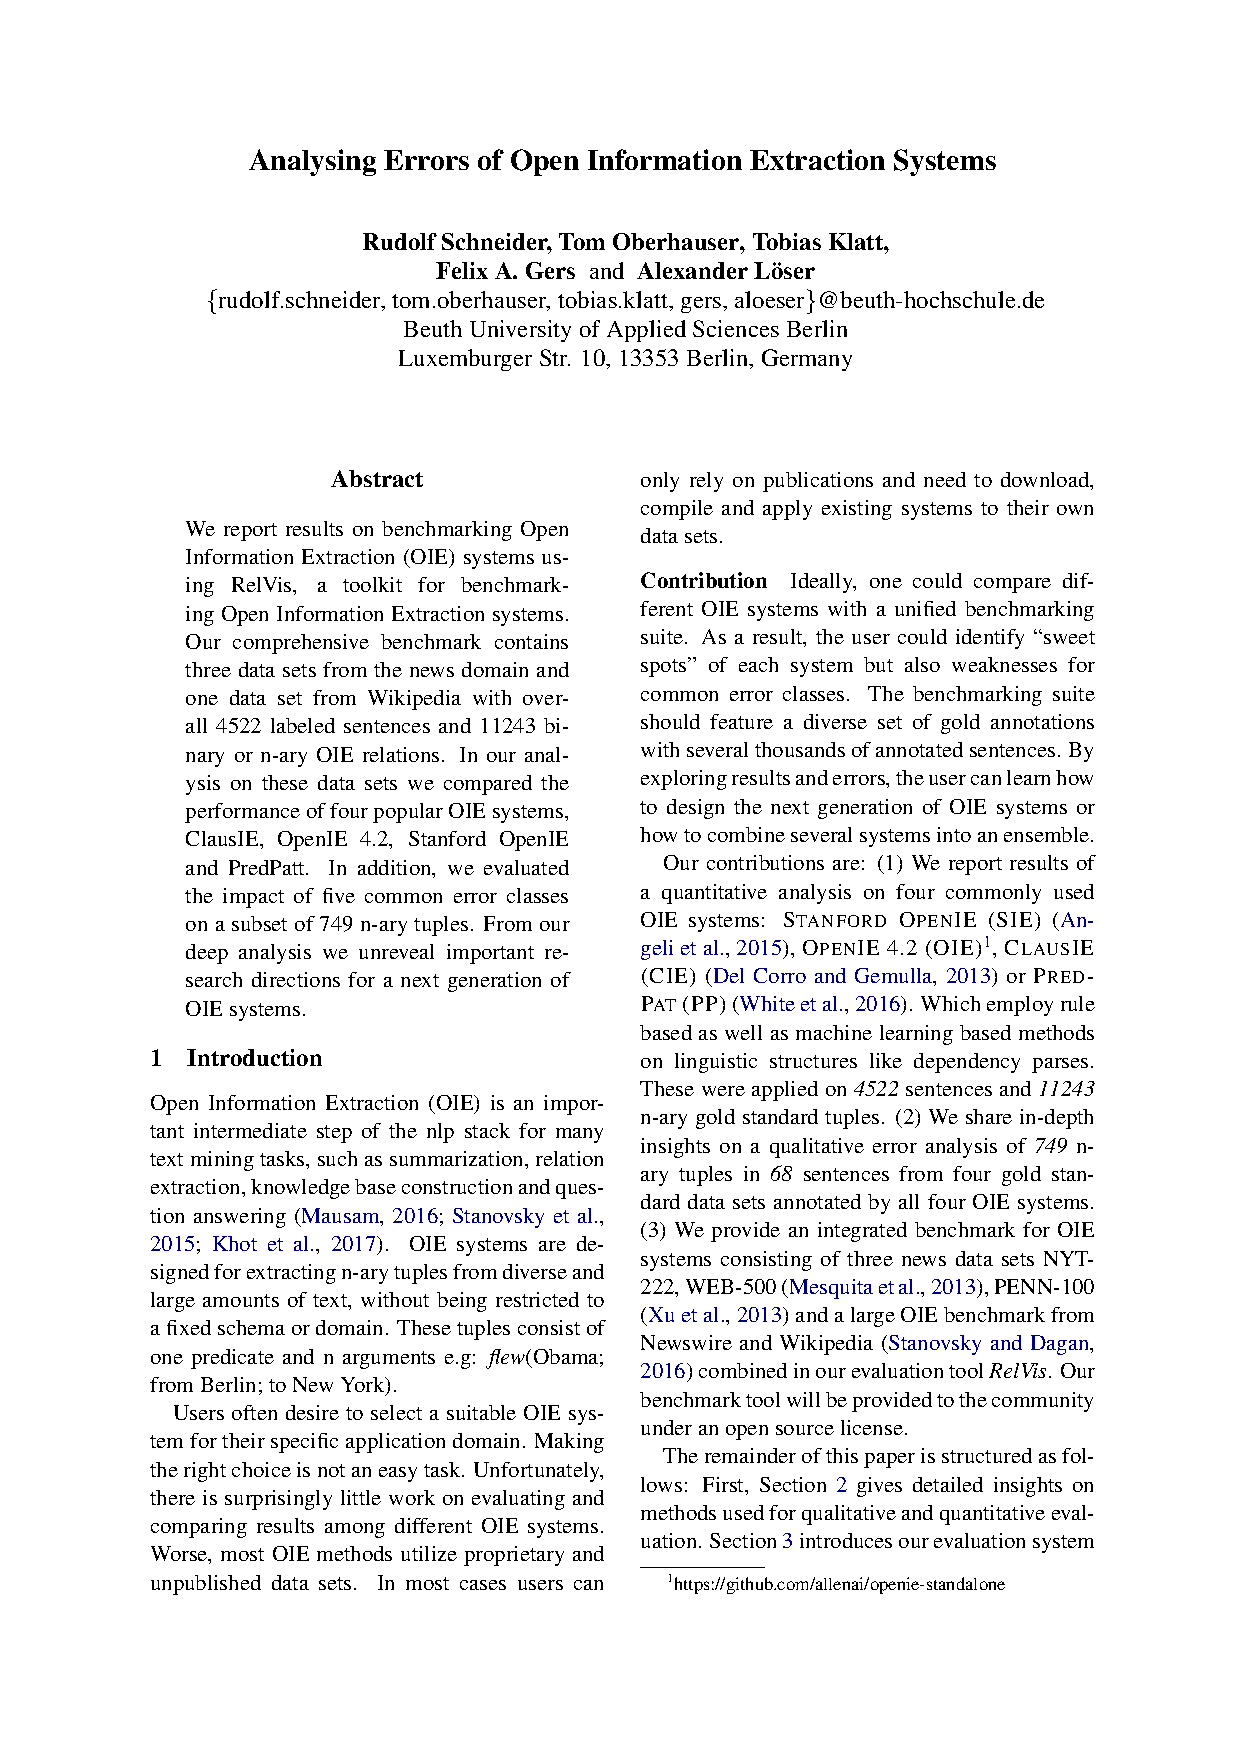
\includepdf[pages=1,addtotoc={1,chapter,1,{Traversal-Free Word Vector Evaluation in Analogy Space},ref:paper_1}]{final/1/1_Paper.pdf}
\ClearShipoutPicture
\includepdf[pages=2-]{final/1/1_Paper.pdf}
\index{Gurnani, Nishant}
\citeinfo{6}{10}
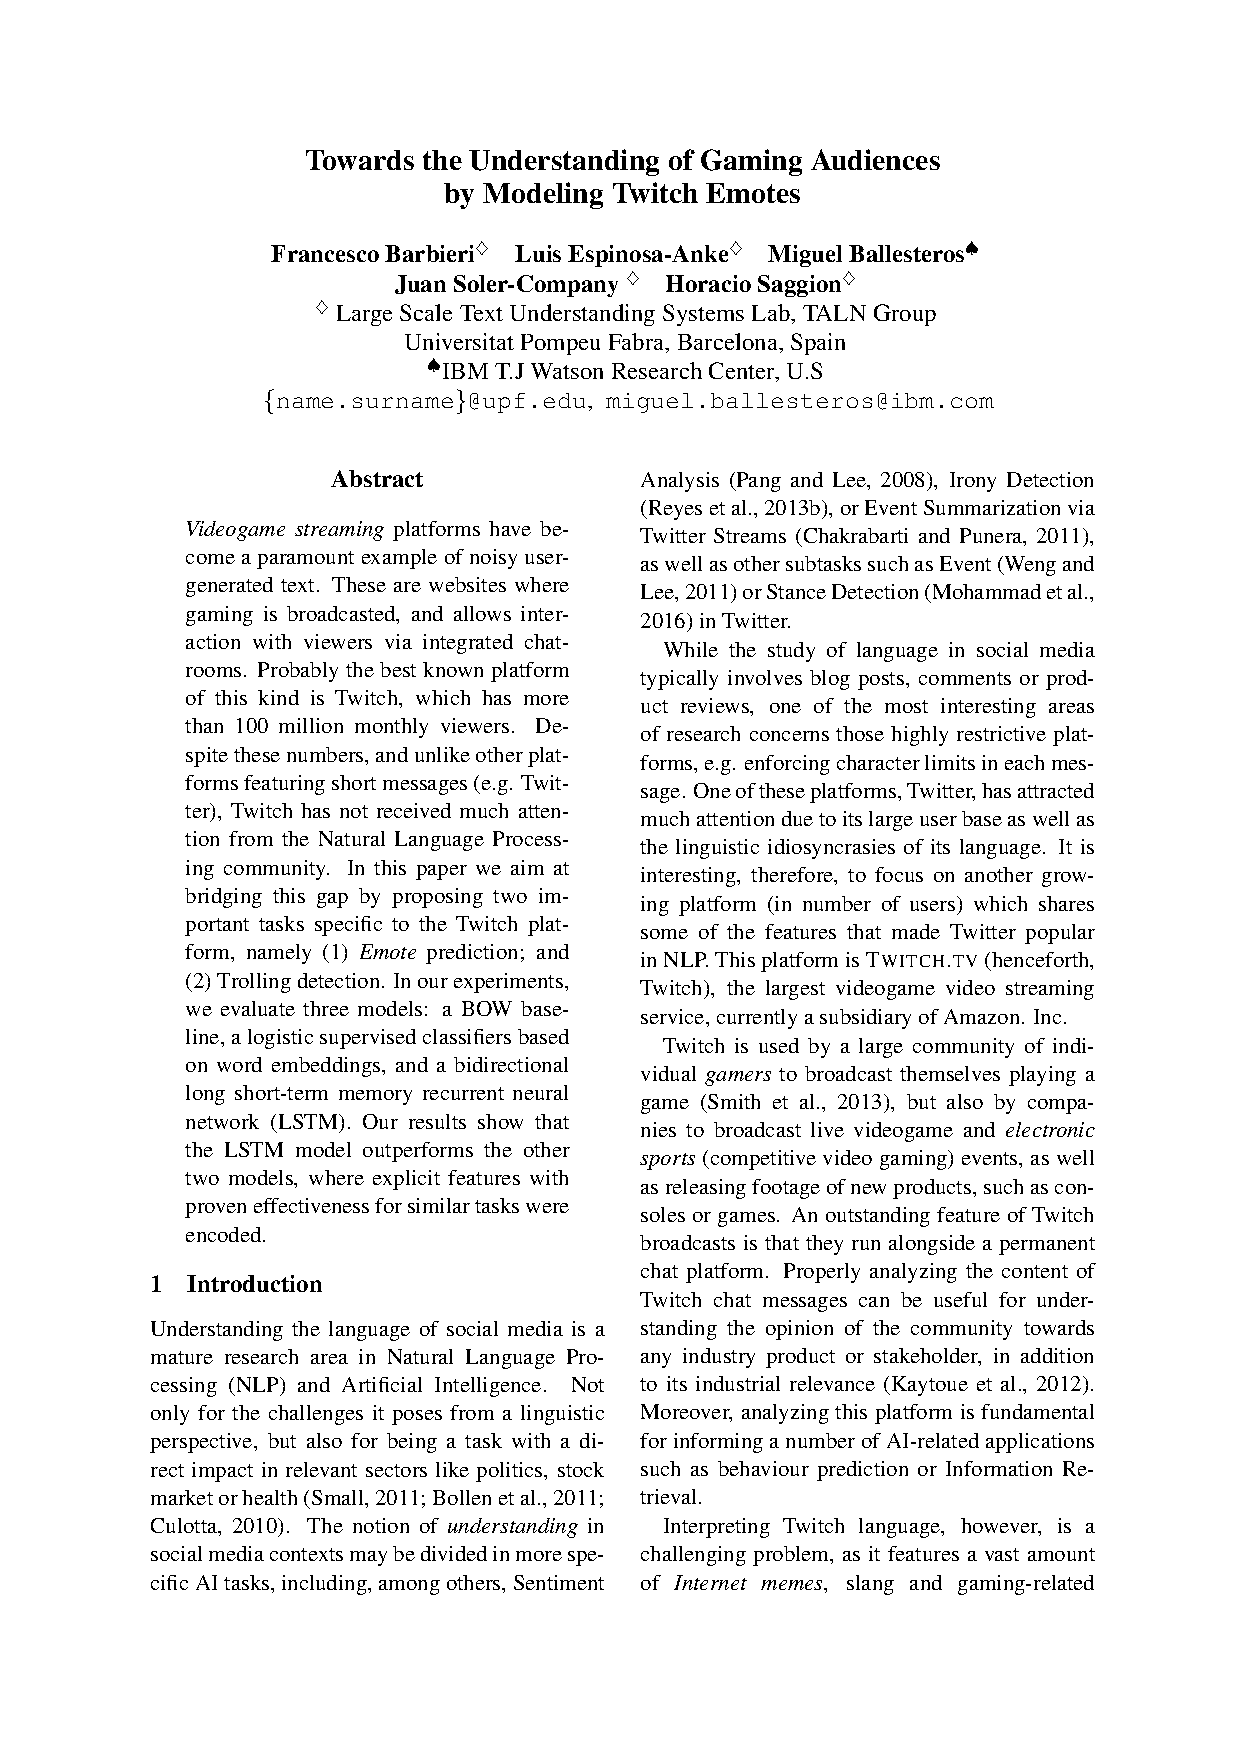
\includepdf[pages=1,addtotoc={1,chapter,1,{Hypothesis Testing based Intrinsic Evaluation of Word Embeddings},ref:paper_4}]{final/4/4_Paper.pdf}
\ClearShipoutPicture
\includepdf[pages=2-]{final/4/4_Paper.pdf}
\index{Auguste, Jeremy}
\index{Rey, Arnaud}
\index{Favre, Benoit}
\citeinfo{11}{16}
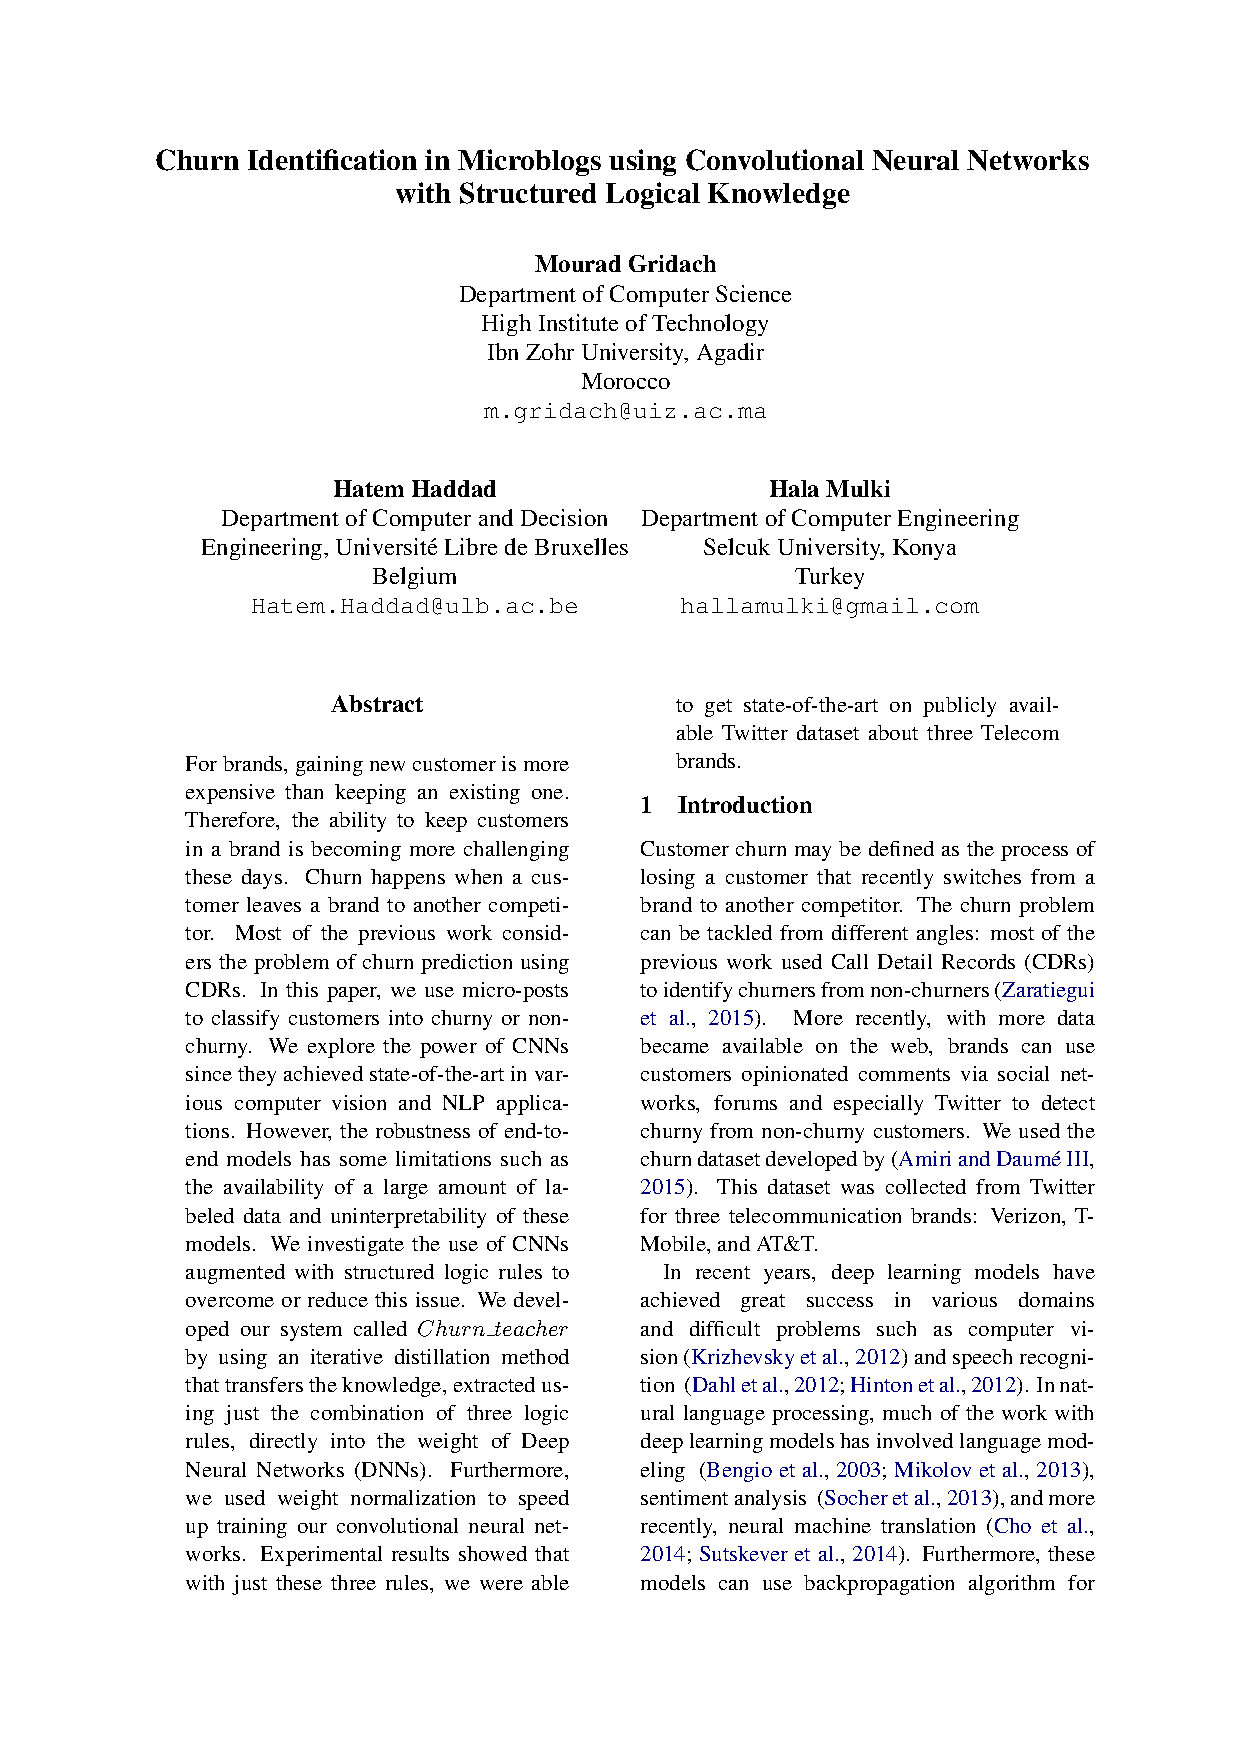
\includepdf[pages=1,addtotoc={1,chapter,1,{Evaluation of word embeddings against cognitive processes: primed reaction times in lexical decision and naming tasks},ref:paper_6}]{final/6/6_Paper.pdf}
\ClearShipoutPicture
\includepdf[pages=2-]{final/6/6_Paper.pdf}
\index{Gulati, Anmol}
\index{Agrawal, Kumar Krishna}
\citeinfo{17}{20}
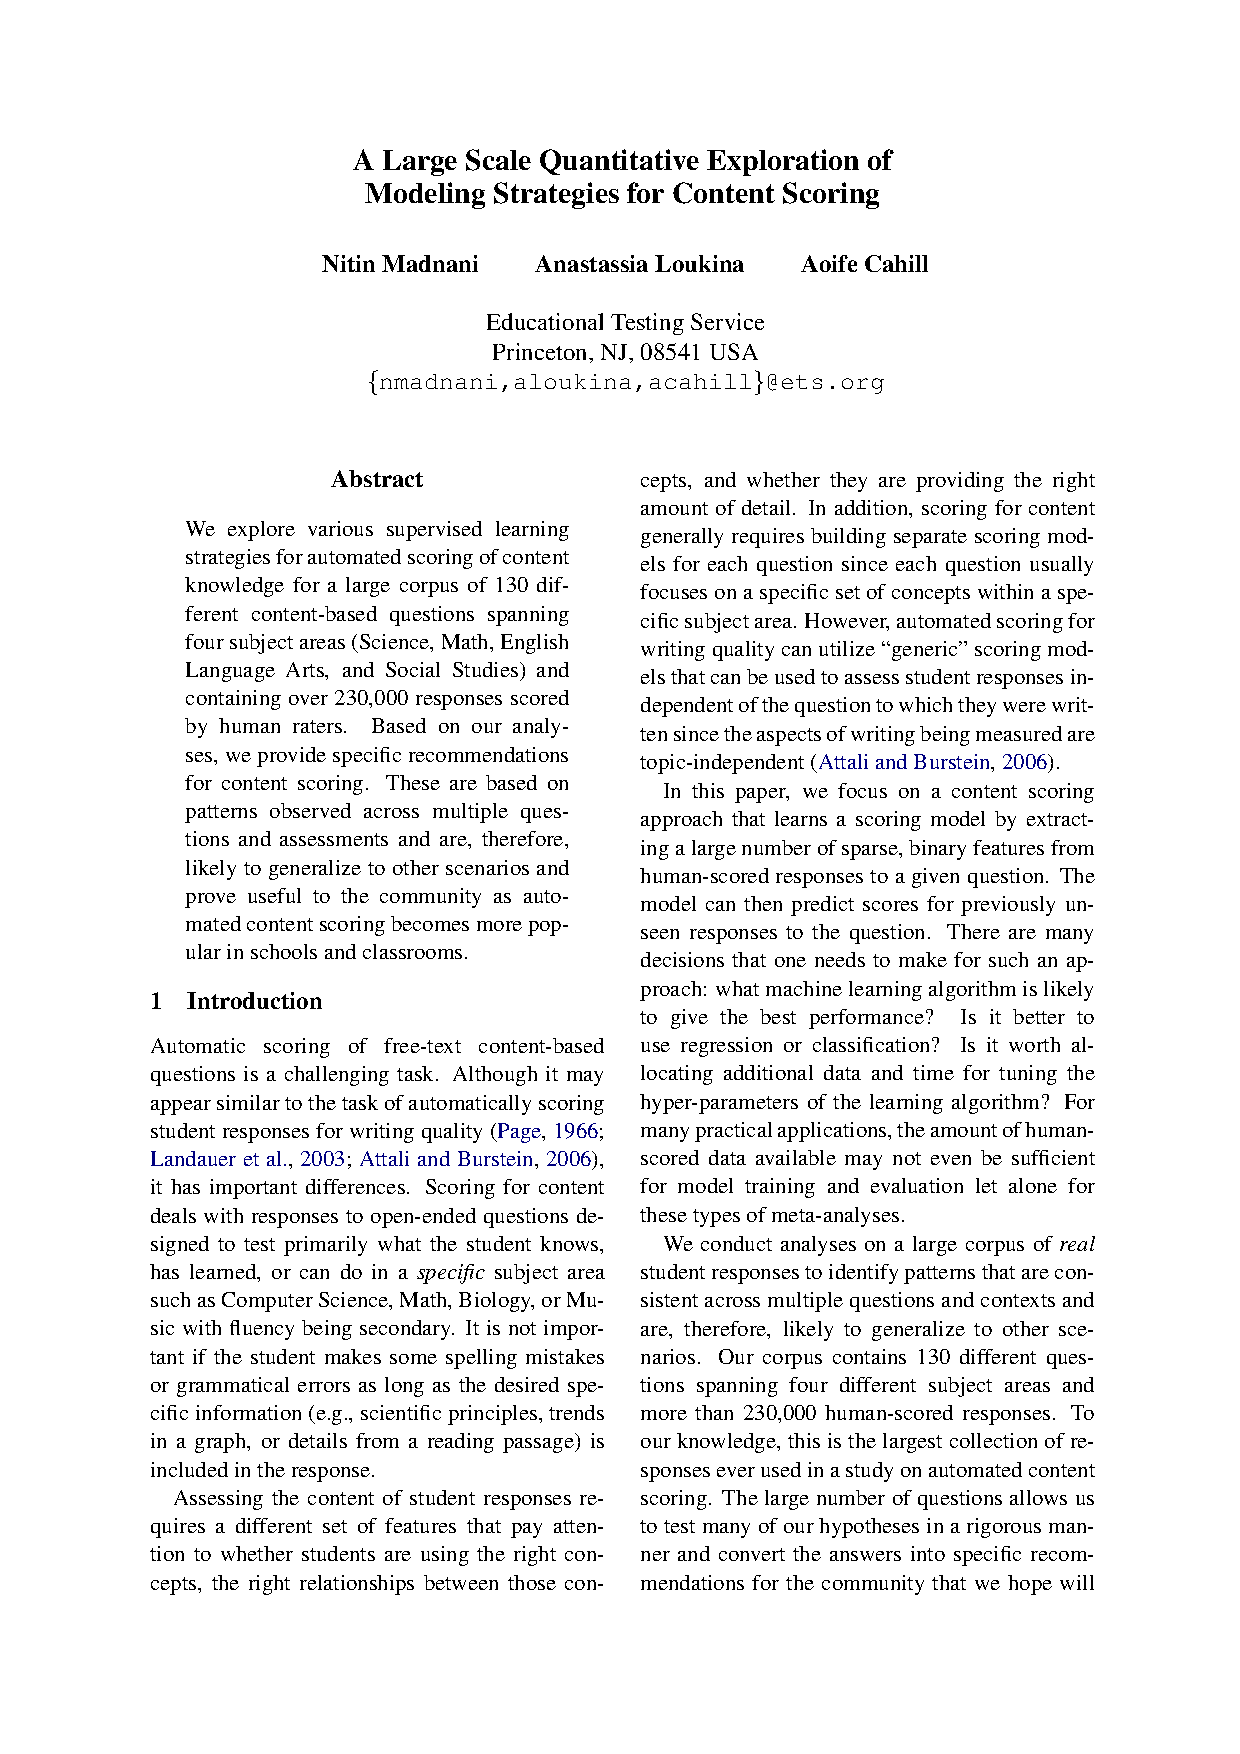
\includepdf[pages=1,addtotoc={1,chapter,1,{Playing with Embeddings : Evaluating embeddings for Robot Language Learning through MUD Games},ref:paper_15}]{final/15/15_Paper.pdf}
\ClearShipoutPicture
\includepdf[pages=2-]{final/15/15_Paper.pdf}
\index{Sulea, Octavia-Maria@\c{S}ulea, Octavia-Maria}
\citeinfo{21}{25}
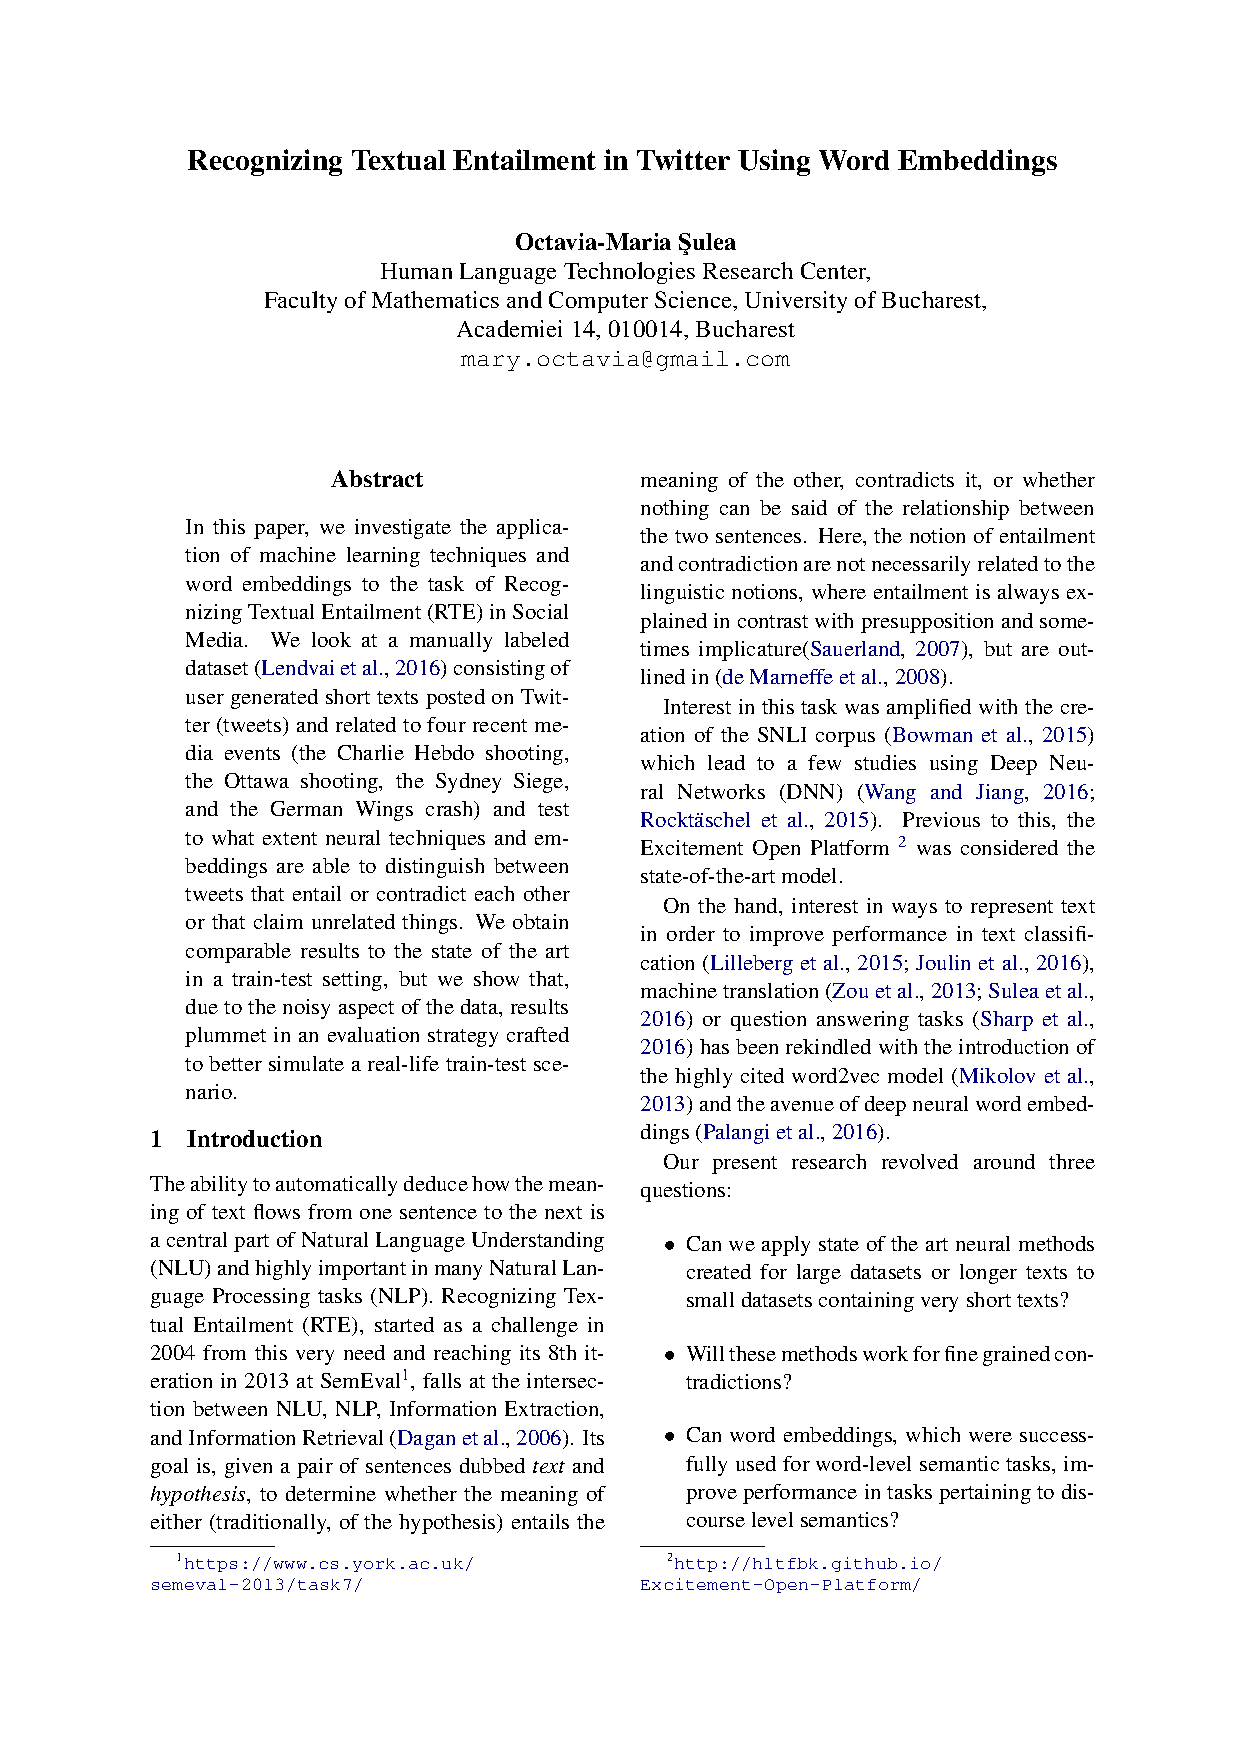
\includepdf[pages=1,addtotoc={1,chapter,1,{Recognizing Textual Entailment in Twitter Using Word Embeddings},ref:paper_5}]{final/5/5_Paper.pdf}
\ClearShipoutPicture
\includepdf[pages=2-]{final/5/5_Paper.pdf}
\index{Chen, Qian}
\index{Zhu, Xiaodan}
\index{Ling, Zhen-Hua}
\index{Wei, Si}
\index{Jiang, Hui}
\index{Inkpen, Diana}
\citeinfo{26}{30}
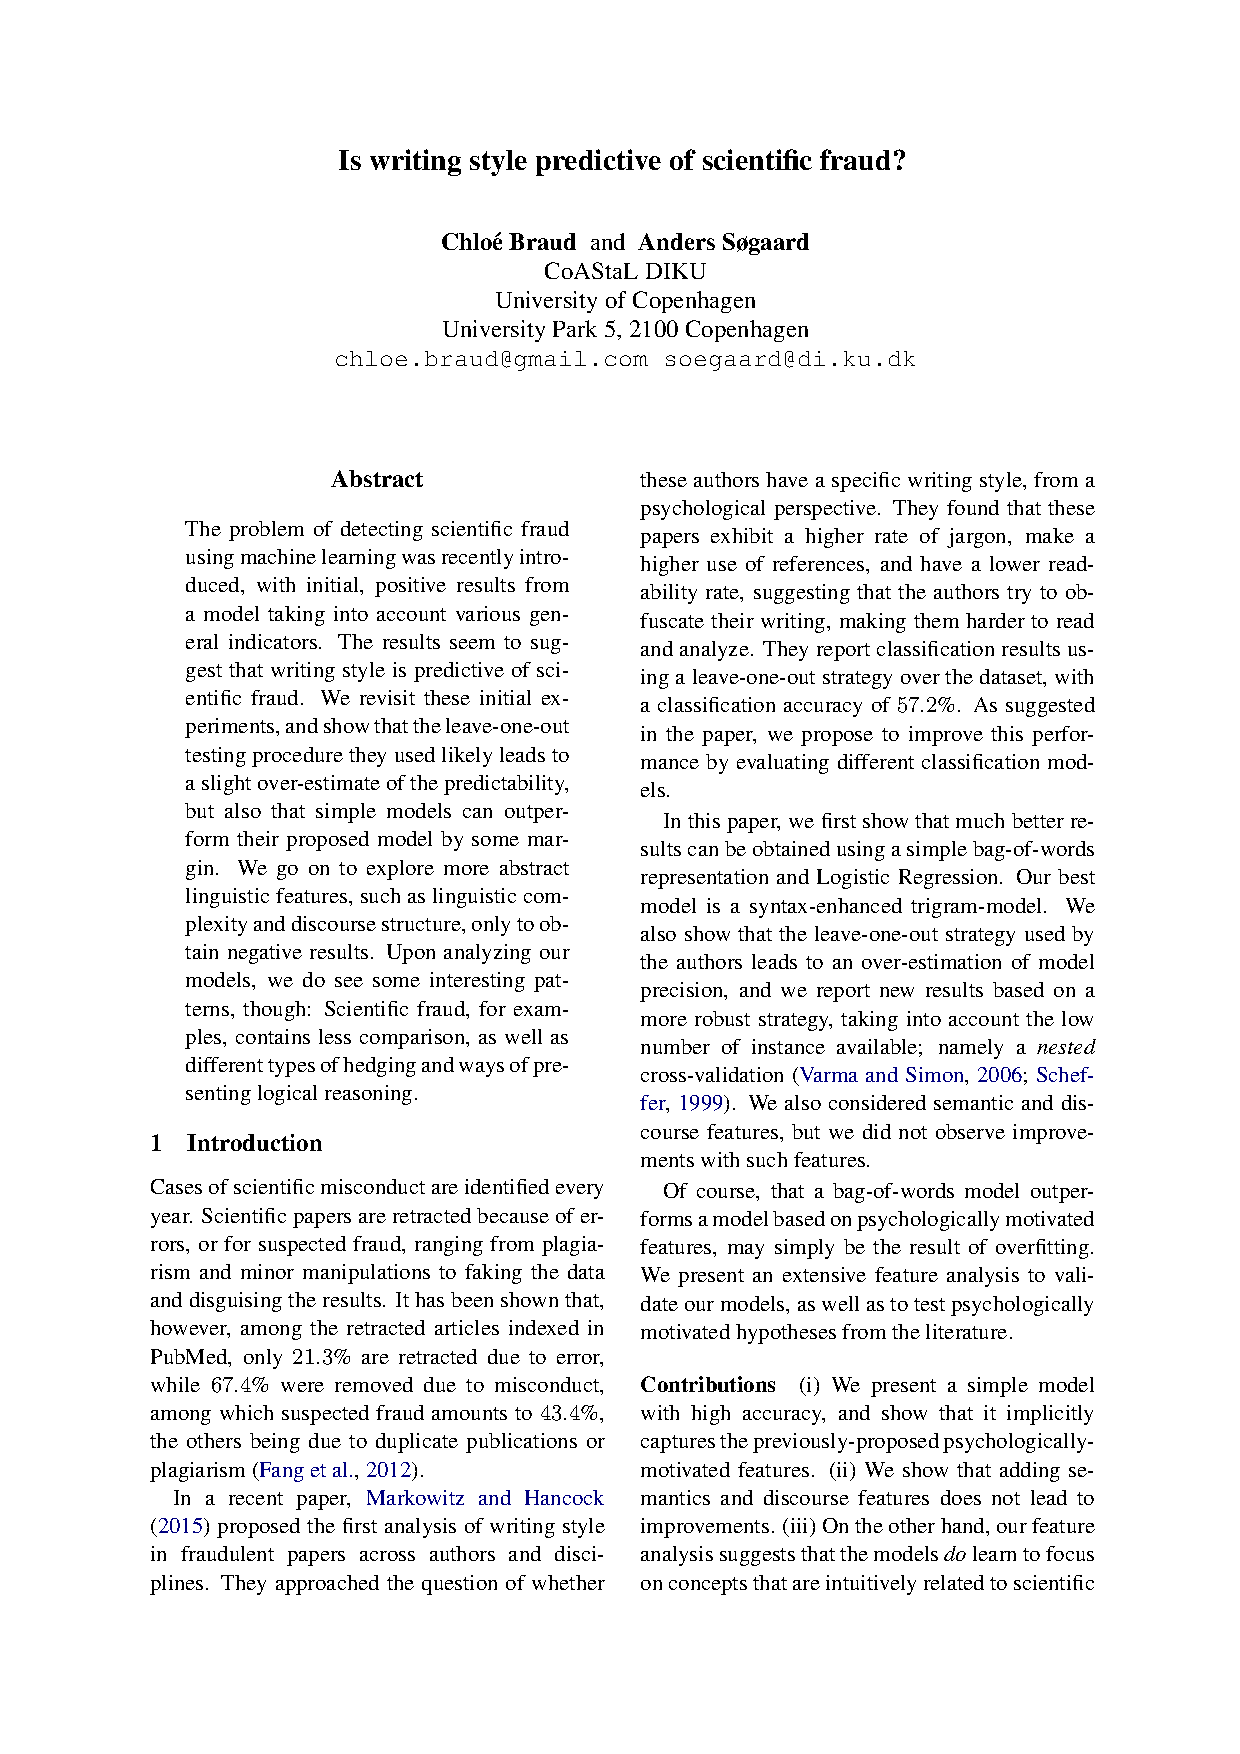
\includepdf[pages=1,addtotoc={1,chapter,1,{Recurrent Neural Network-Based Sentence Encoder with Gated Attention for Natural Language Inference},ref:paper_7}]{final/7/7_Paper.pdf}
\ClearShipoutPicture
\includepdf[pages=2-]{final/7/7_Paper.pdf}
\index{Nie, Yixin}
\index{Bansal, Mohit}
\citeinfo{31}{35}
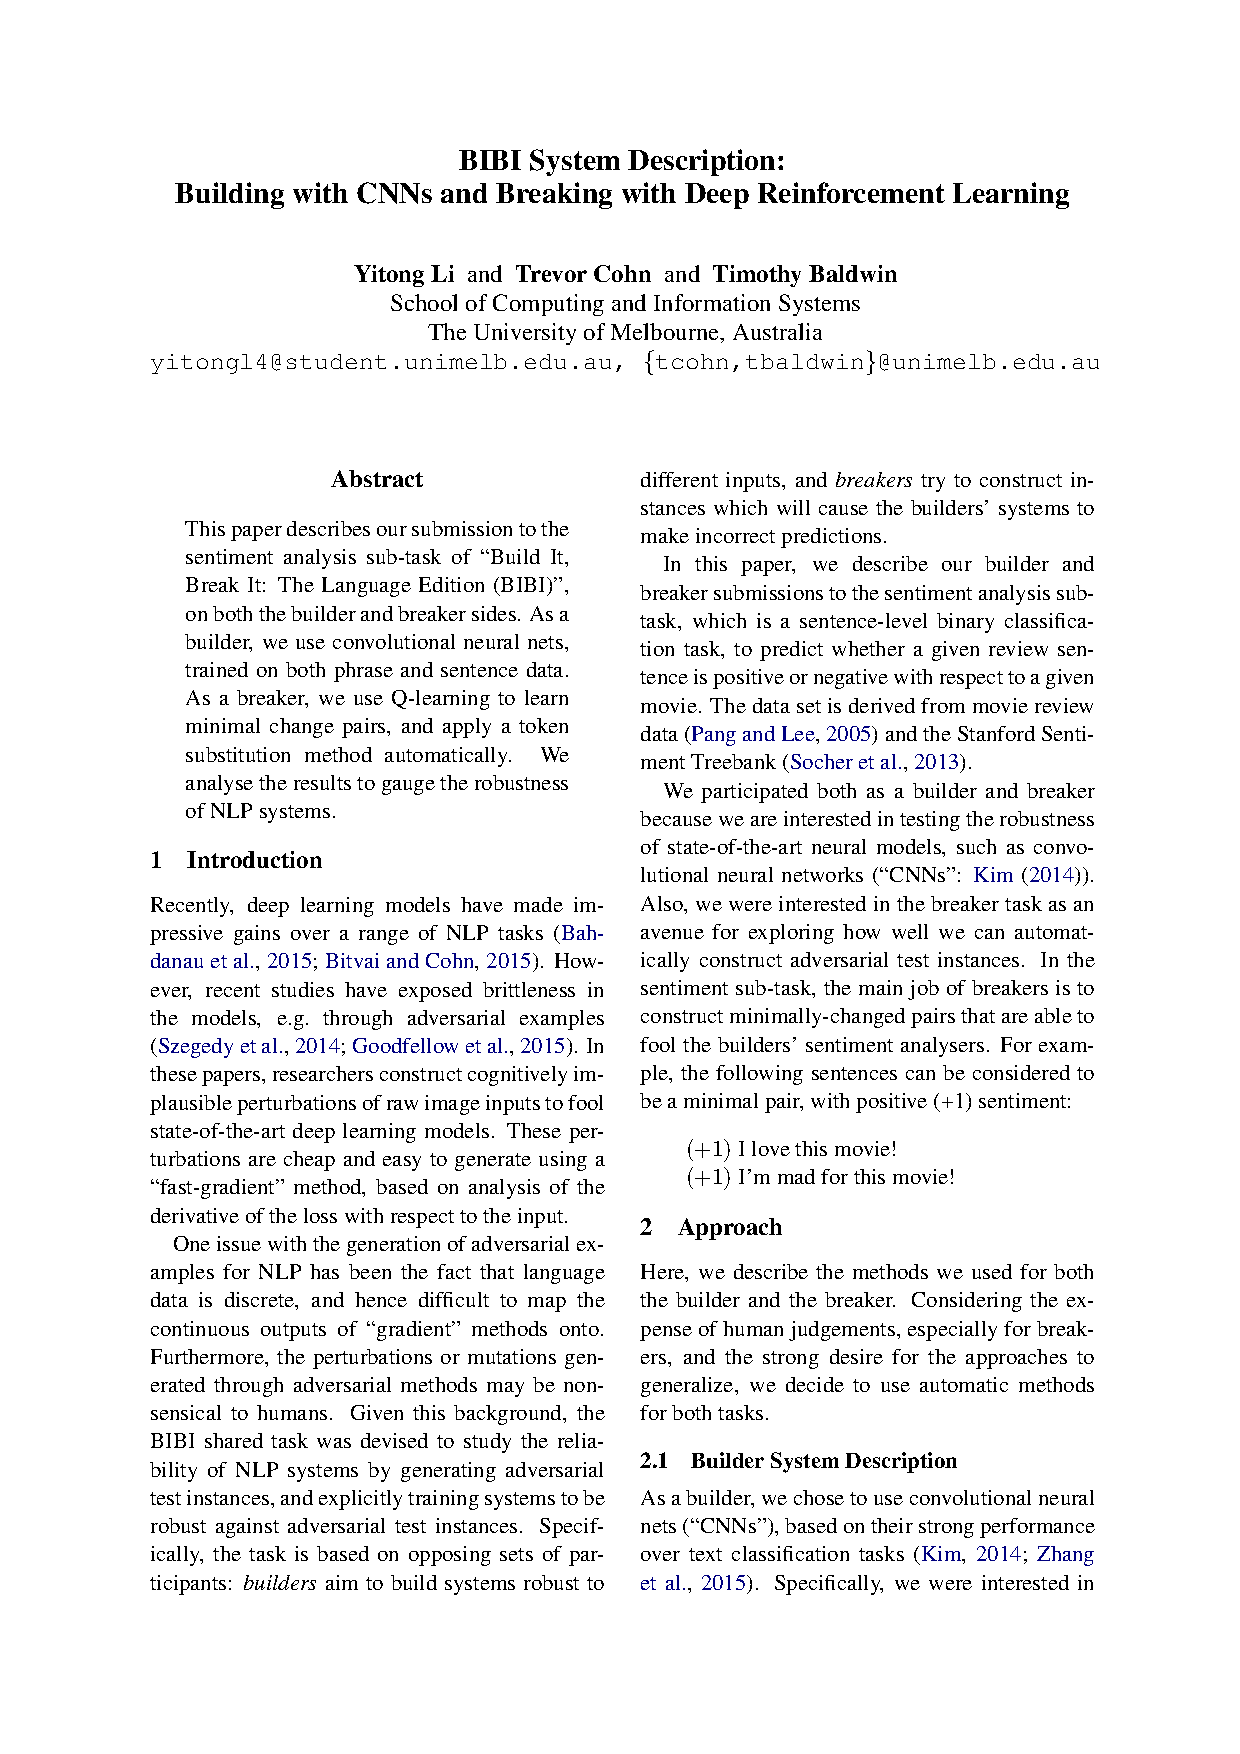
\includepdf[pages=1,addtotoc={1,chapter,1,{Shortcut-Stacked Sentence Encoders for Multi-Domain Inference},ref:paper_10}]{final/10/10_Paper.pdf}
\ClearShipoutPicture
\includepdf[pages=2-]{final/10/10_Paper.pdf}
\index{Yang, Han}
\index{Costa-jussa, Marta R.@Costa-juss\`{a}, Marta R.}
\index{Fonollosa, Jose A. R.@Fonollosa, Jos\'{e} A. R.}
\citeinfo{36}{40}
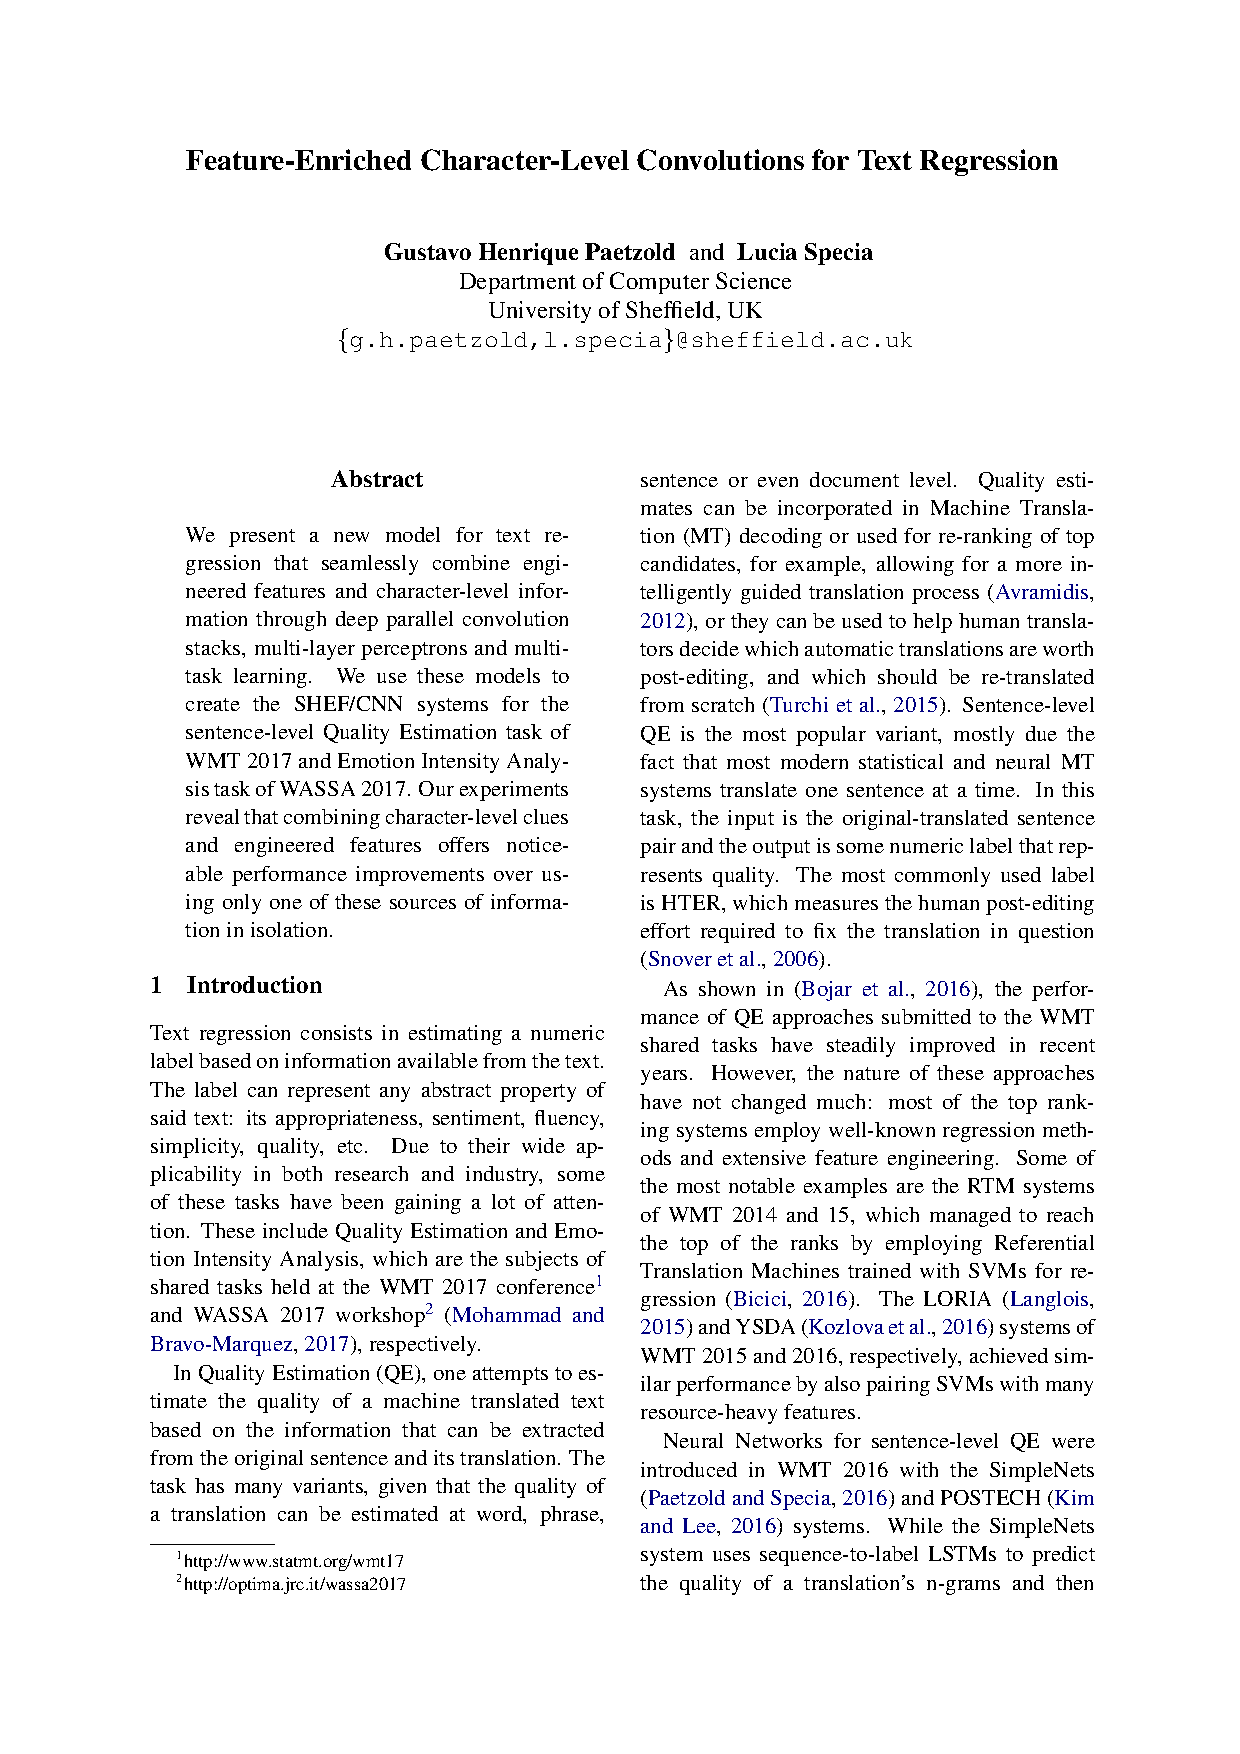
\includepdf[pages=1,addtotoc={1,chapter,1,{Character-level Intra Attention Network for Natural Language Inference},ref:paper_3}]{final/3/3_Paper.pdf}
\ClearShipoutPicture
\includepdf[pages=2-]{final/3/3_Paper.pdf}
\index{Balazs, Jorge}
\index{Marrese-Taylor, Edison}
\index{Loyola, Pablo}
\index{Matsuo, Yutaka}
\citeinfo{41}{45}
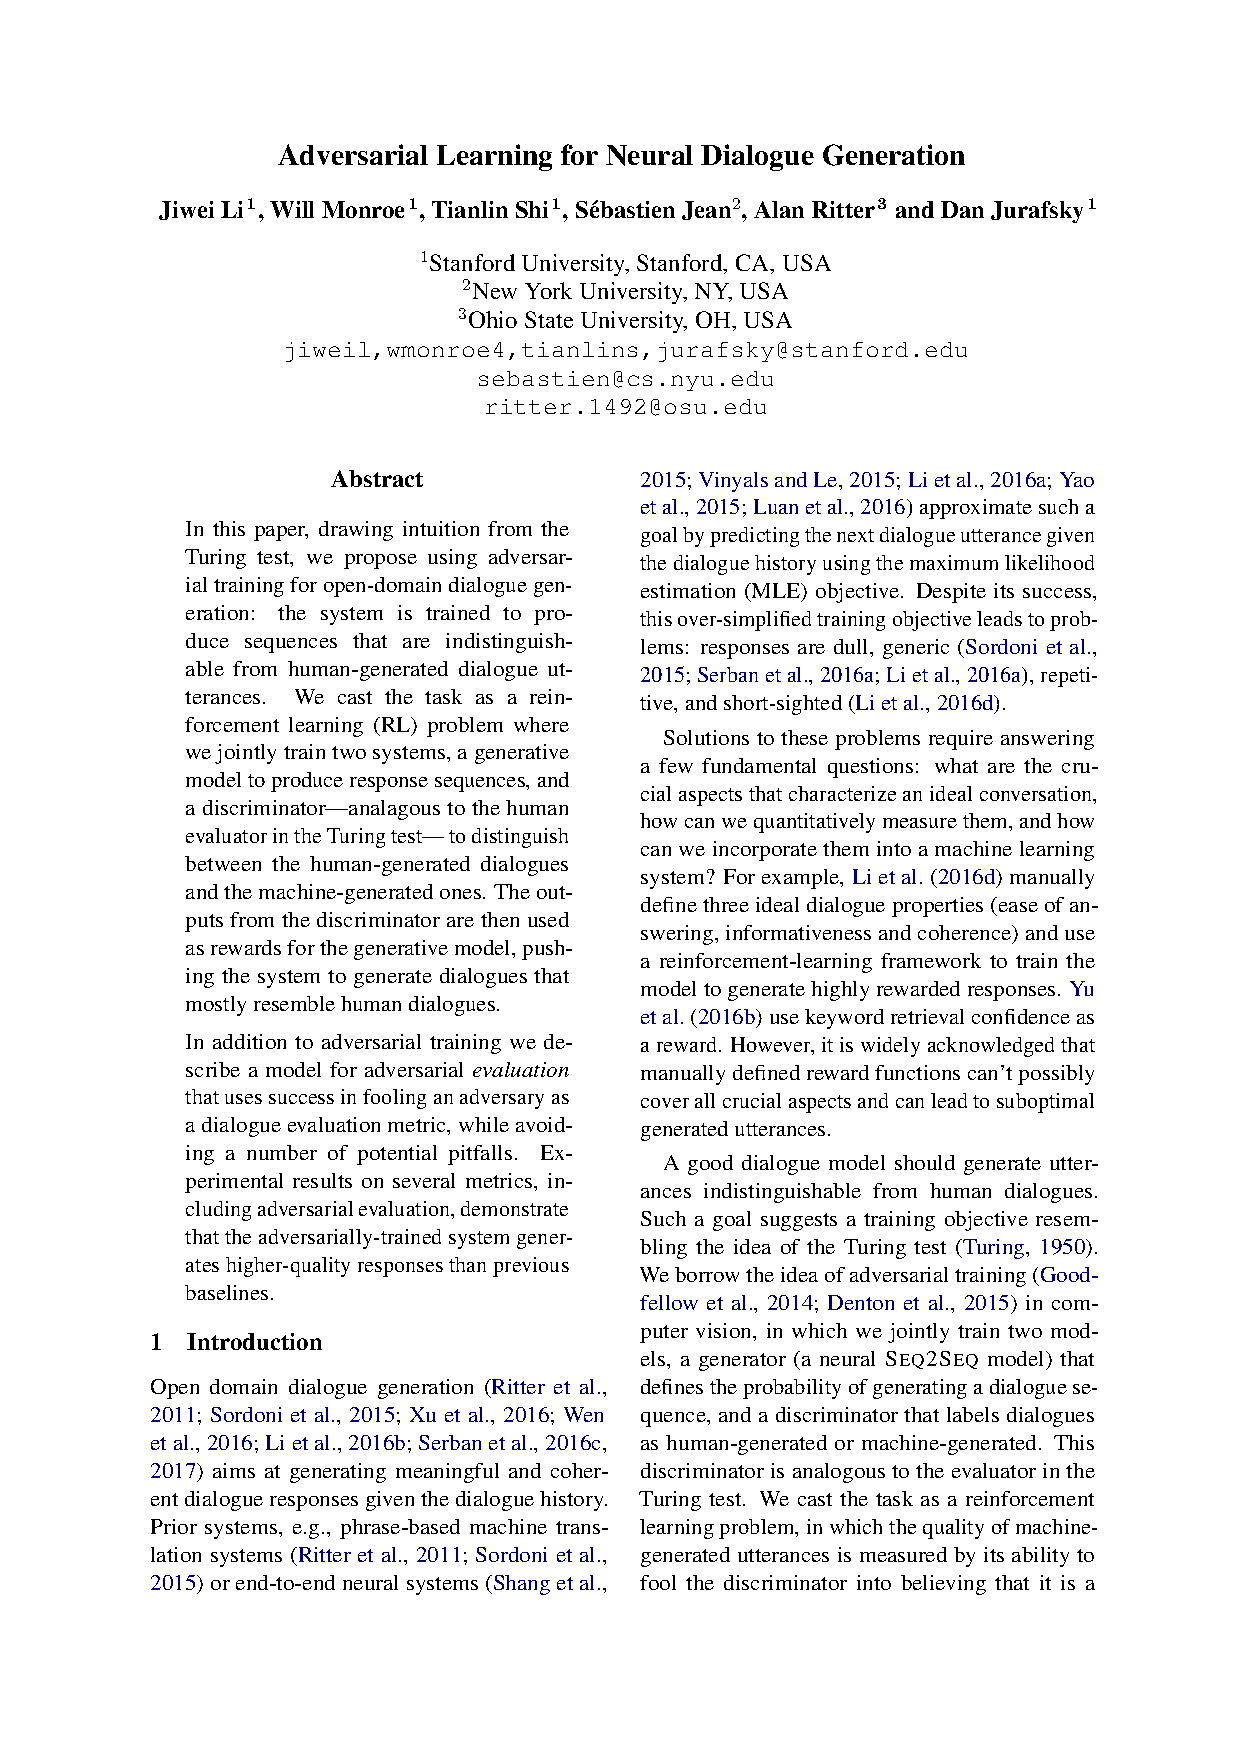
\includepdf[pages=1,addtotoc={1,chapter,1,{Refining Raw Sentence Representations for Textual Entailment Recognition via Attention},ref:paper_11}]{final/11/11_Paper.pdf}
\ClearShipoutPicture
\includepdf[pages=2-]{final/11/11_Paper.pdf}
\index{Vu, Hoa}
\citeinfo{46}{50}
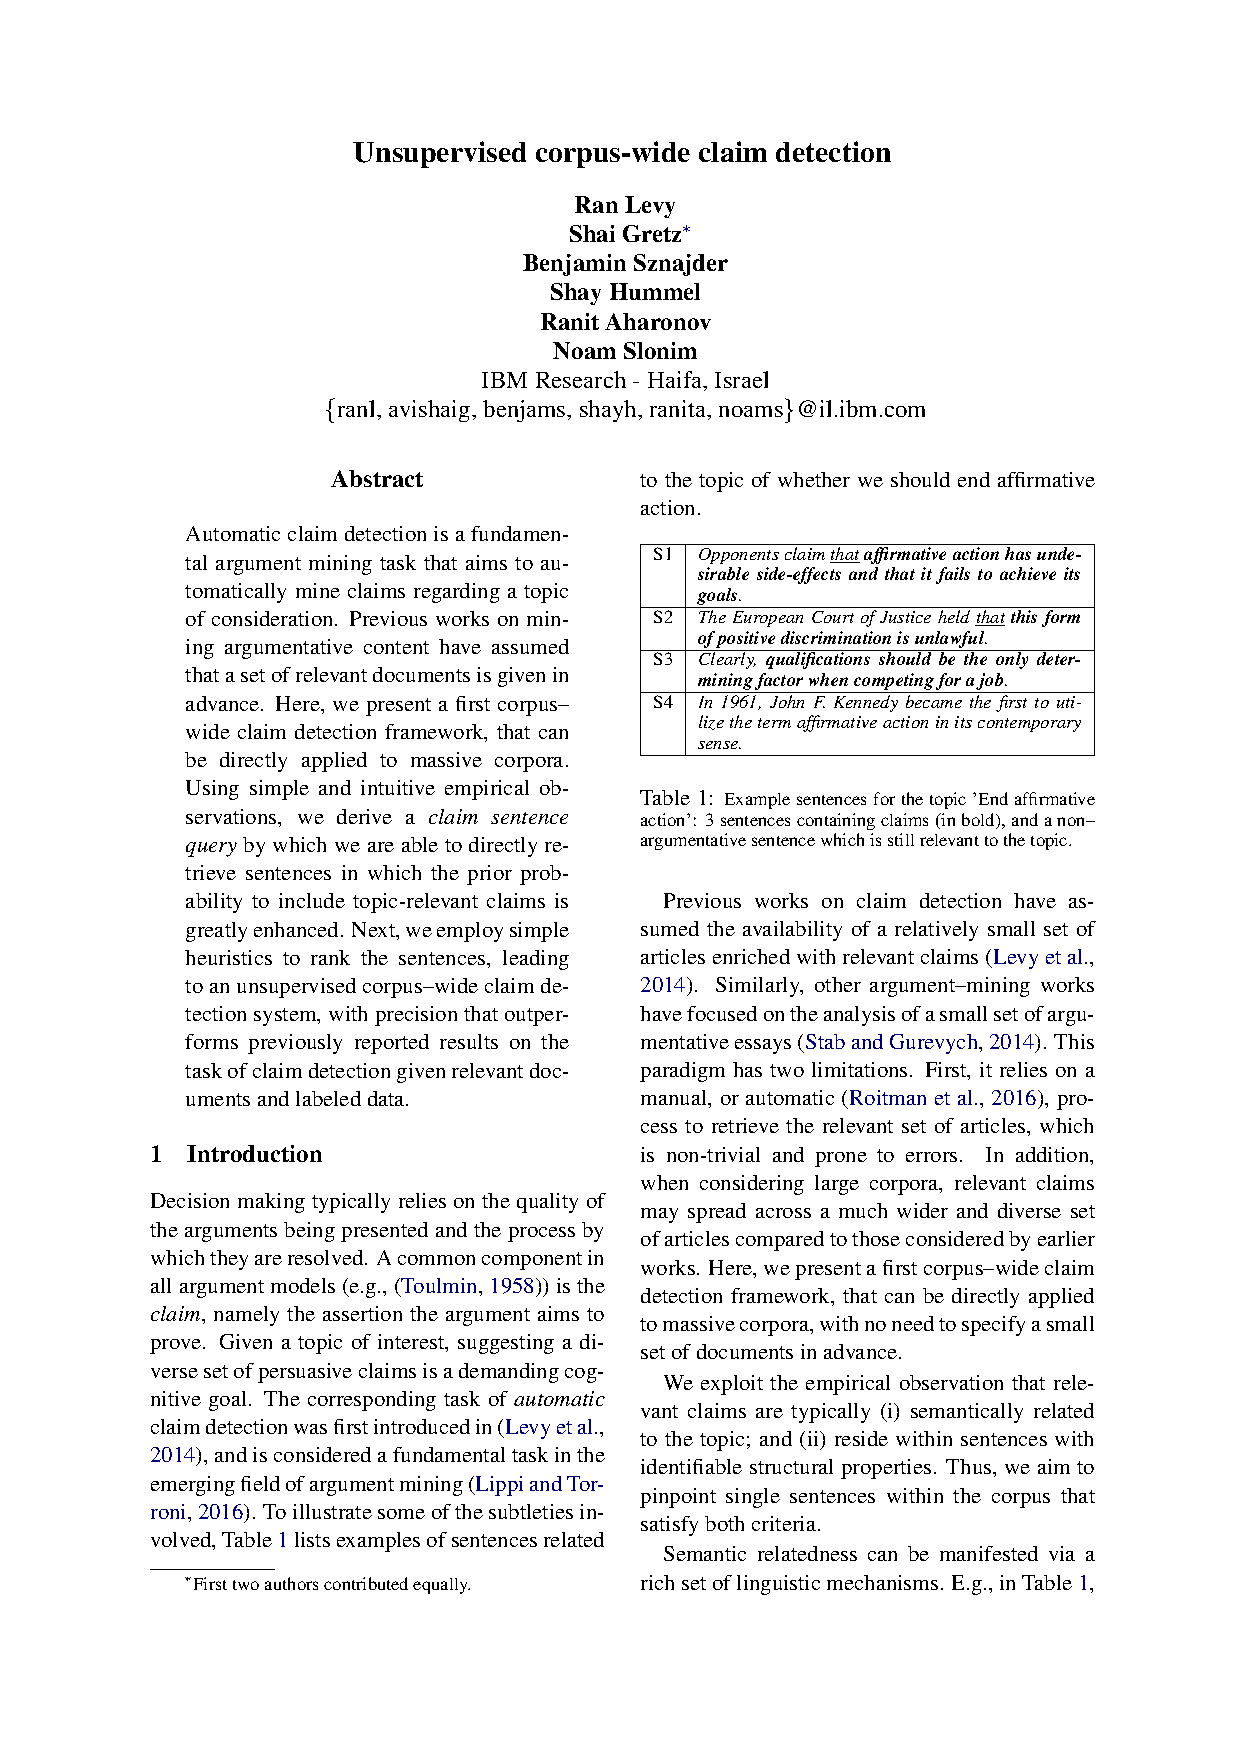
\includepdf[pages=1,addtotoc={1,chapter,1,{LCT-MALTA's Submission to RepEval 2017 Shared Task},ref:paper_14}]{final/14/14_Paper.pdf}
\ClearShipoutPicture
\includepdf[pages=2-]{final/14/14_Paper.pdf}
   % automatically generated from DB file

% -------- END MATTER: AUTHOR INDEX --------

\ifthenelse{\equal{\draftflag}{1}}{}{
  \ifthenelse{\isodd{\value{page}}}{}
    {\newpage \thispagestyle{empty} \phantom{.}}
  \pagestyle{empty}
  \printindex
}

\end{document}